\documentclass[a4paper,11pt,fleqn,dvipsnames,twoside,openright]{memoir} 	% Openright aabner kapitler paa hoejresider (openany begge)

%%%% PACKAGES %%%%

% ¤¤ Oversaettelse og tegnsaetning ¤¤ %
\usepackage[utf8]{inputenc}					% Input-indkodning af tegnsaet (UTF8)
\usepackage[danish]{babel}					% Dokumentets sprog
\usepackage[T1]{fontenc}					% Output-indkodning af tegnsaet (T1)
\usepackage{ragged2e,anyfontsize}			% Justering af elementer
\usepackage{fixltx2e}						% Retter forskellige fejl i LaTeX-kernen
																			
% ¤¤ Figurer og tabeller (floats) ¤¤ %
\usepackage{graphicx} 						% Haandtering af eksterne billeder (JPG, PNG, EPS, PDF)
%\usepackage{eso-pic}						% Tilfoej billedekommandoer paa hver side
%\usepackage{wrapfig}						% Indsaettelse af figurer omsvoebt af tekst. \begin{wrapfigure}{Placering}{Stoerrelse}
\usepackage{multirow}                		% Fletning af raekker og kolonner (\multicolumn og \multirow)
\usepackage{multicol}         	        	% Muliggoer output i spalter
\usepackage{rotating}						% Rotation af tekst med \begin{sideways}...\end{sideways}
\usepackage{colortbl} 						% Farver i tabeller (fx \columncolor og \rowcolor)
\usepackage{xcolor}							% Definer farver med \definecolor. Se mere: http://en.wikibooks.org/wiki/LaTeX/Colors
\usepackage{flafter}						% Soerger for at floats ikke optraeder i teksten foer deres reference
\let\newfloat\relax 						% Justering mellem float-pakken og memoir
\usepackage{float}							% Muliggoer eksakt placering af floats, f.eks. \begin{figure}[H]

% ¤¤ Matematik mm. ¤¤
\usepackage{amsmath,amssymb,stmaryrd} 		% Avancerede matematik-udvidelser
\usepackage{mathtools,mathabx}
\newcommand\ARN[1]{\makebox[0pt][l]{$#1$}\kern-0.15em\raisebox{1.5ex}{$\curvearrowright$}}
\newcommand\ALN[1]{\makebox[0pt][l]{$#1$}\kern-0.15em\raisebox{1.5ex}{$\curvearrowleft$}}
\newcommand\AR[1]{\makebox[0pt][l]{$#1$}\kern0.0em\raisebox{1.5ex}{$\curvearrowright$}}
\newcommand\AL[1]{\makebox[0pt][l]{$#1$}\kern0.0em\raisebox{1.5ex}{$\curvearrowleft$}}						% Andre matematik- og tegnudvidelser
\usepackage{textcomp}                 		% Symbol-udvidelser (f.eks. promille-tegn med \textperthousand )
\usepackage{rsphrase}						% Kemi-pakke til RS-saetninger, f.eks. \rsphrase{R1}
\usepackage[version=3]{mhchem} 				% Kemi-pakke til flot og let notation af formler, f.eks. \ce{Fe2O3}
\usepackage{siunitx}						% Flot og konsistent praesentation af tal og enheder med \si{enhed} og \SI{tal}{enhed}
\sisetup{output-decimal-marker = {,}}		% Opsaetning af \SI (DE for komma som decimalseparator) 

% ¤¤ Referencer og kilder ¤¤ %
\usepackage[danish]{varioref}				% Muliggoer bl.a. krydshenvisninger med sidetal (\vref)
\usepackage{natbib}							% Udvidelse med naturvidenskabelige citationsmodeller
%\usepackage{xr}							% Referencer til eksternt dokument med \externaldocument{<NAVN>}
%\usepackage{glossaries}					% Terminologi- eller symbolliste (se mere i Daleifs Latex-bog)

% ¤¤ Misc. ¤¤ %
\usepackage{listings}						% Placer kildekode i dokumentet med \begin{lstlisting}...\end{lstlisting}
\usepackage{lipsum}							% Dummy text \lipsum[..]
\usepackage[shortlabels]{enumitem}			% Muliggoer enkelt konfiguration af lister
\usepackage{pdfpages}						% Goer det muligt at inkludere pdf-dokumenter med kommandoen \includepdf[pages={x-y}]{fil.pdf}	
\pdfoptionpdfminorversion=6					% Muliggoer inkludering af pdf dokumenter, af version 1.6 og hoejere
\pretolerance=2500 							% Justering af afstand mellem ord (hoejt tal, mindre orddeling og mere luft mellem ord)

% Kommentarer og rettelser med \fxnote. Med 'final' i stedet for 'draft' udloeser hver note en error i den faerdige rapport.
\usepackage[footnote,draft,danish,silent,nomargin]{fixme}		


%%%% CUSTOM SETTINGS %%%%

% ¤¤ Marginer ¤¤ %
\setlrmarginsandblock{3.5cm}{2.5cm}{*}		% \setlrmarginsandblock{Indbinding}{Kant}{Ratio}
\setulmarginsandblock{2.5cm}{3.0cm}{*}		% \setulmarginsandblock{Top}{Bund}{Ratio}
\checkandfixthelayout 						% Oversaetter vaerdier til brug for andre pakker

%	¤¤ Afsnitsformatering ¤¤ %
\setlength{\parindent}{0mm}           		% Stoerrelse af indryk
\setlength{\parskip}{3mm}          			% Afstand mellem afsnit ved brug af double Enter
\linespread{1,1}							% Linie afstand

% ¤¤ Litteraturlisten ¤¤ %
\bibpunct[,]{[}{]}{;}{a}{,}{,} 				% Definerer de 6 parametre ved Harvard henvisning (bl.a. parantestype og seperatortegn)
\bibliographystyle{bibtex/harvard}			% Udseende af litteraturlisten.

% ¤¤ Indholdsfortegnelse ¤¤ %
\setsecnumdepth{subparagraph}		 			% Dybden af nummerede overkrifter (part/chapter/section/subsection)
\maxsecnumdepth{subparagraph}					% Dokumentklassens graense for nummereringsdybde
\settocdepth{subparagraph} 					% Dybden af indholdsfortegnelsen

% ¤¤ Lister ¤¤ %
\setlist{
  topsep=0pt,								% Vertikal afstand mellem tekst og listen
  itemsep=-1ex,								% Vertikal afstand mellem items
} 

% ¤¤ Visuelle referencer ¤¤ %
\usepackage[colorlinks]{hyperref}			% Danner klikbare referencer (hyperlinks) i dokumentet.
\hypersetup{colorlinks = true,				% Opsaetning af farvede hyperlinks (interne links, citeringer og URL)
    linkcolor = black,
    citecolor = black,
    urlcolor = black
}

% ¤¤ Opsaetning af figur- og tabeltekst ¤¤ %
\captionnamefont{\small\bfseries\itshape}	% Opsaetning af tekstdelen ('Figur' eller 'Tabel')
\captiontitlefont{\small}					% Opsaetning af nummerering
\captiondelim{. }							% Seperator mellem nummerering og figurtekst
\hangcaption								% Venstrejusterer flere-liniers figurtekst under hinanden
\captionwidth{\linewidth}					% Bredden af figurteksten
\setlength{\belowcaptionskip}{0pt}			% Afstand under figurteksten
		
% ¤¤ Opsaetning af listings ¤¤ %

\definecolor{commentGreen}{RGB}{34,139,24}
\definecolor{stringPurple}{RGB}{208,76,239}

\lstset{language=Matlab,					% Sprog
	basicstyle=\ttfamily\scriptsize,		% Opsaetning af teksten
	keywords={for,if,while,else,elseif,		% Noegleord at fremhaeve
			  end,break,return,case,
			  switch,function},
	keywordstyle=\color{blue},				% Opsaetning af noegleord
	commentstyle=\color{commentGreen},		% Opsaetning af kommentarer
	stringstyle=\color{stringPurple},		% Opsaetning af strenge
	showstringspaces=false,					% Mellemrum i strenge enten vist eller blanke
	numbers=left, numberstyle=\tiny,		% Linjenumre
	extendedchars=true, 					% Tillader specielle karakterer
	columns=flexible,						% Kolonnejustering
	breaklines, breakatwhitespace=true,		% Bryd lange linjer
}

% ¤¤ Navngivning ¤¤ %
\addto\captionsdanish{
	\renewcommand\appendixname{Appendiks}
	\renewcommand\contentsname{Indholdsfortegnelse}	
	\renewcommand\appendixpagename{Appendiks}
	\renewcommand\appendixtocname{Appendiks}
	\renewcommand\cftchaptername{\chaptername~}				% Skriver "Kapitel" foran kapitlerne i indholdsfortegnelsen
	\renewcommand\cftappendixname{\appendixname~}			% Skriver "Appendiks" foran appendiks i indholdsfortegnelsen
}

% ¤¤ Kapiteludssende ¤¤ %
\definecolor{numbercolor}{gray}{0.7}		% Definerer en farve til brug til kapiteludseende
\newif\ifchapternonum

\makechapterstyle{jenor}{					% Definerer kapiteludseende frem til ...
  \renewcommand\beforechapskip{0pt}
  \renewcommand\printchaptername{}
  \renewcommand\printchapternum{}
  \renewcommand\printchapternonum{\chapternonumtrue}
  \renewcommand\chaptitlefont{\fontfamily{pbk}\fontseries{db}\fontshape{n}\fontsize{25}{35}\selectfont\raggedleft}
  \renewcommand\chapnumfont{\fontfamily{pbk}\fontseries{m}\fontshape{n}\fontsize{1in}{0in}\selectfont\color{numbercolor}}
  \renewcommand\printchaptertitle[1]{%
    \noindent
    \ifchapternonum
    \begin{tabularx}{\textwidth}{X}
    {\let\\\newline\chaptitlefont ##1\par} 
    \end{tabularx}
    \par\vskip-2.5mm\hrule
    \else
    \begin{tabularx}{\textwidth}{Xl}
    {\parbox[b]{\linewidth}{\chaptitlefont ##1}} & \raisebox{-15pt}{\chapnumfont \thechapter}
    \end{tabularx}
    \par\vskip2mm\hrule
    \fi
  }
}											% ... her

\chapterstyle{jenor}						% Valg af kapiteludseende - Google 'memoir chapter styles' for alternativer

% ¤¤ Sidehoved ¤¤ %

\makepagestyle{AAU}							% Definerer sidehoved og sidefod udseende frem til ...
\makepsmarks{AAU}{%
	\createmark{chapter}{left}{shownumber}{}{. \ }
	\createmark{section}{right}{shownumber}{}{. \ }
	\createplainmark{toc}{both}{\contentsname}
	\createplainmark{lof}{both}{\listfigurename}
	\createplainmark{lot}{both}{\listtablename}
	\createplainmark{bib}{both}{\bibname}
	\createplainmark{index}{both}{\indexname}
	\createplainmark{glossary}{both}{\glossaryname}
}
\nouppercaseheads											% Ingen Caps oenskes

\makeevenhead{AAU}{Gruppe B149}{}{\leftmark}				% Definerer lige siders sidehoved (\makeevenhead{Navn}{Venstre}{Center}{Hoejre})
\makeoddhead{AAU}{\rightmark}{}{Aalborg Universitet}		% Definerer ulige siders sidehoved (\makeoddhead{Navn}{Venstre}{Center}{Hoejre})
\makeevenfoot{AAU}{\thepage}{}{}							% Definerer lige siders sidefod (\makeevenfoot{Navn}{Venstre}{Center}{Hoejre})
\makeoddfoot{AAU}{}{}{\thepage}								% Definerer ulige siders sidefod (\makeoddfoot{Navn}{Venstre}{Center}{Hoejre})
\makeheadrule{AAU}{\textwidth}{0.5pt}						% Tilfoejer en streg under sidehovedets indhold
\makefootrule{AAU}{\textwidth}{0.5pt}{1mm}					% Tilfoejer en streg under sidefodens indhold

\copypagestyle{AAUchap}{AAU}								% Sidehoved for kapitelsider defineres som standardsider, men med blank sidehoved
\makeoddhead{AAUchap}{}{}{}
\makeevenhead{AAUchap}{}{}{}
\makeheadrule{AAUchap}{\textwidth}{0pt}
\aliaspagestyle{chapter}{AAUchap}							% Den ny style vaelges til at gaelde for chapters
															% ... her
															
\pagestyle{AAU}												% Valg af sidehoved og sidefod


%%%% CUSTOM COMMANDS %%%%

% ¤¤ Billede hack ¤¤ %
\newcommand{\figur}[4]{
		\begin{figure}[H] \centering
			\includegraphics[width=#1\textwidth]{billeder/#2}
			\caption{#3}\label{#4}
		\end{figure} 
}

% ¤¤ Specielle tegn ¤¤ %
\newcommand{\decC}{^{\circ}\text{C}}
\newcommand{\dec}{^{\circ}}
\newcommand{\m}{\cdot}


%%%% ORDDELING %%%%

\hyphenation{}											% Preamble indlaeses
\raggedbottom													% Soerger for at LaTeX ikke "straekker" teksten

%\includeonly{file1,file2}										% Inkluder kun specifikke filer (kommasepareret liste)

\begin{document}												% Starter dokumentet - obligatorisk

%\setlength\parindent{15pt}
\frontmatter													% Forindhold - nummereres med romertal

\thispagestyle{empty}
\begin{flushright}
\vspace{3cm}

\phantom{hul}

\phantom{hul}

\phantom{hul}

\textsl{\Huge FUNDERING AF TILBYGNING AF STRØYBERGS PALÆ} \\ \vspace{1cm}

\rule{13cm}{3mm} \\ \vspace{1.5cm}
\vspace{1cm}

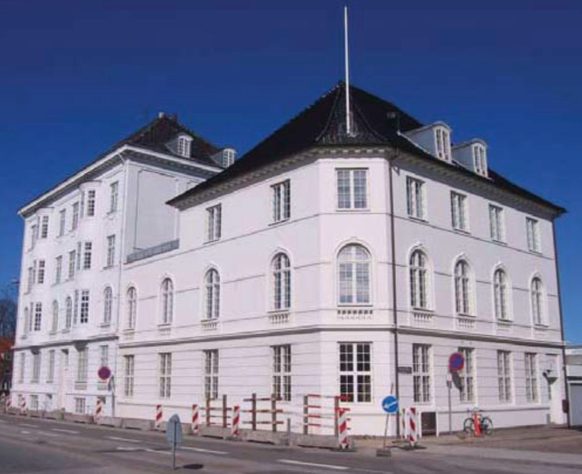
\includegraphics[width=0.9\textwidth]{billeder/forside.png}

\vspace{2cm} 
\textsc{\Large P2 Projekt - Modellernes virkelighed \\
Gruppe B149 \\
Byggeri \& Anlæg\\
Aalborg Universitet\\
D. 27. maj 2015\\}
\end{flushright}

\cleardoublepage												% Indsaetter tom side, saa naeste kapitel starter paa hoejre side (hvis noedvendigt)
% Dette er LaTeX-versionen af titelbladet for TNB studenterrapporter
% Filen kræver:
% Universitetets logo:  AAU-logo-stud-UK eller AAU-logo-stud-DK
% Synopsis: En fil ved navn synopsis.tex

% Udarbejdet af: Jesper Nørgaard (jesper@noergaard.eu) 10. april 2012

\phantomsection
\pdfbookmark[0]{Titelblad}{titelblad}
\thispagestyle{empty}

\begin{minipage}[t]{0.48\textwidth}
\vspace*{-25pt}			%\vspace*{-9pt}

\includegraphics[height=4cm]{billeder/AAU-logo-stud-DK-RGB}
\end{minipage}
\hfill
\begin{minipage}[t]{0.48\textwidth}
{\small 
\textbf{Første Studieår v/ Det Teknisk-}\\
\textbf{Naturvidenskabelige Fakultet}  \\
Byggeri og Anlæg \\
Strandvejen 12-14 \\
9000 Aalborg \\
http://www.tnb.aau.dk}
\end{minipage}

\vspace*{1cm}

\begin{minipage}[t]{0.48\textwidth}
\textbf{Titel:} \\[5pt]\bigskip\hspace{2ex}


\textbf{Projekt:} \\[5pt]\bigskip\hspace{2ex}
P2-projekt - Modellernes virkelighed

\textbf{Projektperiode:} \\[5pt]\bigskip\hspace{2ex}
Februar 2015 - Maj 2015

\textbf{Projektgruppe:} \\[5pt]\bigskip\hspace{2ex}
B149

\textbf{Deltagere:} \\[5pt]\hspace*{2ex}
Jacob Scharling Jørgensen \\\hspace*{2ex}
Karoline Vestergaard Hansen \\\hspace*{2ex}
Katrine Nørgaard Reberholt \\\hspace*{2ex}
Marc Lund Nielsen \\\hspace*{2ex}
Michael Elgaard Mortensen \\\hspace*{2ex}
Morten Rask Jensen \\\hspace*{2ex}
Nikolaj Skov Gravesen \\\bigskip\hspace{2ex}

\textbf{Vejledere:} \\[5pt]\hspace*{2ex}
Katrine Raabjerg Meltoft \\\hspace*{2ex}
Gitte \\\hspace*{2ex}
Johan \\\bigskip\hspace{2ex}

\vspace*{0.5cm}

\textbf{Oplagstal: 9} \\
\textbf{Sidetal: 79} \\
\textbf{Bilag: 4} \\ 
\textbf{Afsluttet 27-05-2015}

\end{minipage}
\hfill
\begin{minipage}[t]{0.483\textwidth}
Synopsis: \\[5pt]
\fbox{\parbox{7cm}{\bigskipDette P2-projekt omhandler den ene tilbygning til Strøybergs Palæ.
\newline
\newline
Strøybergs Palæ ligger placeret ved havnen i Aalborg og er placeret inden for en fremlagt vækstakse. Bygningen skal laves henfør lokalplan 1-1-107. Projektet beskriver tilbygningen ud fra to perspektiver; en kontekstuel del, hvor der lægges fokus på Aalborgs udvikling gennemtiden, og dens nuværende og planlagte udvikling, heriblandt den fremlagte vækstakse. Der vil blive redegjort for disse og diskuteret om den planlagte udvikling overhovedet er realistisk. Den tekniske del vil have fokus på dimensioneringen af tilbygningen og dens fundament. Der vil blive redegjort for Aalborgs geologi og forskellige jordarters udseende og styrke. Udfra dette vil der blive angivet en fundamenttype og udregnet størrelsen af det, så fundamentet har tilstrækkelig bæreevne til dimensioneringen af tilbygningen.
\bigskip}}
\end{minipage}

\vfill

{\footnotesize\itshape Rapportens indhold er frit tilgængeligt, men offentliggørelse (med kildeangivelse) må kun ske efter aftale med forfatterne.}

% Rapportens indhold er frit tilgængeligt, men offentliggørelse (med kildeangivelse) må kun ske efter aftale med forfatterne.
% The content of the report is freely available, but publication (with source reference) may only take place in agreement with the authors.

\cleardoublepage
\chapter*{Forord}
Denne rapport er udarbejdet af gruppe B149, en gruppe 2. semesters studerende på Byggeri og Anlæg uddannelsen ved Aalborg Universitet. \textit{Modellernes Virkelighed} er det overordnede tema for projektet, med undertemaet \textit{Vækstaksen i Aalborg}. Projektet omhandler en tilbygning ved Strøybergs Palæ.
\\
\\
Der rettes stor tak til vejledere Gitte Lyng Grønbech, Johan Clausen og Katrine Rabjerg Meltofte for vejledning og konstruktiv kritik. 
\\
\\
\textbf{Læsevejledning}
\newline
Der vil igennem rapporten fremtræde kildehenvisninger, og disse vil være samlet i en kildeliste bagest i rapporten. Der er i rapporten anvendt kildehenvisning efter Harvardmetoden. Denne henvisning fører til kildelisten, hvor bøger er angivet med forfatter, titel, udgave og forslag, mens internetsider er angivet med forfatter, titel og dato. Figurer og tabeller er nummereret i henhold til kapitel, dvs. den første figur i kapitel 7 har nummer 7.1, den anden nummer 7.2, osv. De samlede beregninger kan findes på hjemmesiden www.markhaurum.com, da der kun vil findes eksempler og korte uddrag af beregningerne i rapporten.


\phantom{Luft}

\phantom{Luft}

\begin{table}[H]
	\centering
		\begin{tabular}{c c c}
			\underline{\phantom{mmmmmmmmmmmmmm}} & \underline{\phantom{mmmmmmmmmmmmmm}} & \underline{\phantom{mmmmmmmmmmmmmm}} \\
			Jacob Scharling Jørgensen			& Karoline Vestergaard Hansen 		& Katrine Nørgaard Reberholt 			\\
			&&\\
			&&\\
			\underline{\phantom{mmmmmmmmmmmmmm}} & \underline{\phantom{mmmmmmmmmmmmmm}} & \underline{\phantom{mmmmmmmmmmmmmm}} \\
			Marc Lund Nielsen			& Michael Elgaard Mortensen 		& Morten Rask Jensen 				\\
			&&\\
			&&\\
		& \underline{\phantom{mmmmmmmmmmmmmm}} 	&			\\														
		& Nikolaj Skov Gravesen 							& 					
		\end{tabular}
\end{table}
\cleardoublepage

%%%% Indholdsfortegnelse (TOC) %%%%

\phantomsection													% Kunstigt afsnit, som hyperlinks kan 'holde fast i'
\pdfbookmark[0]{Indholdsfortegnelse}{indhold}					% Tildeler en klikbar bookmark til den endelige PDF
\tableofcontents*												% Indholdsfortegnelsen (kaldet ToC) 

%\addtocontents{toc}{\protect\newpage}							% Fremtvinger sideskift i ToC hvis noedvendig (der hvor koden placeres)


\mainmatter														% Hovedindhold - nummereres fra side 1

%%%% Rapportindhold %%%% 										% Rapportindholdet boer IKKE indeholde broedtekst - KUN includede filer!

%% Indledende %%												% Opdel evt. i passende afsnit for overblikkets skyld

\chapter{Indledning}
Aalborg Kommune er med et indbyggertal på over 205.000 og et areal på cirka  1.140 $km^2$, landets tredjestørste kommune målt på indbyggertal og landets anden største kommune målt på areal \citep{indbyggertal}. Det område, som Kommunen dækker, er vist på Figur \ref{fig:aalborgkommune}. 
\newline \indent{     }  Aalborg er en tidligere industriby og førhen var industriområderne placeret i Aalborg Centrum. Nye planer for Aalborg har ført denne industri ud i nogle yderpunkter af Aalborg by. Derfor har kommunen nye visioner om at flytte kultur, studieliv og turisme ind, hvor der før var industri. Kommunens visioner omkring byens udvikling fremgår af Kommuneplanen, hvor det primære fokus i denne rapport vil være et område gennem Aalborg, der er tiltænkt mest vækst, dette betegnes som Vækstaksen (se Figur \ref{fig:vaekstakse}).
\newline \indent{     }  Indenfor de seneste 5-10 år har Aalborgs centrale havnefront gennemgået en stor udvikling. Denne er stadig i gang, hvilket ses ved, at der kommer flere boligbyggerier til havnen, som Strøybergs Palæ er en del af. 
\newline \indent{     }  Det har siden år 2010 været på tale, at lave en tilbygning til den bevaringsværdige bygning, Strøybergs Palæ. Bygningen er fra år 1908 \citep{byggesagen}, beliggende centralt i Aalborg ved Slotspladsen, der er en cirka 200 meter vejstrækning og plads ved Aalborgs centrale havnefront, samt i nærheden af museet Utzon Centret og overfor shoppingcentret Friis. Figur \ref{fig:aalborg} viser Strøybergs Palæs beliggenhed. 
\newline \indent{     }  Når der skal anlægges nye arealer, bygninger, veje osv., skal det opføres i henhold til en lokalplan, der dækker et mindre område inden for kommunen, og har til formål at styre udviklingen indenfor dette område ved hjælp af fastlagte regler og målsætninger. Den gældende lokalplan for området ved Strøybergs Palæ er lokalplan 1-1-107. 

\begin{figure}[htbp] \centering
	\begin{minipage}[b]{0.48\textwidth}\centering
		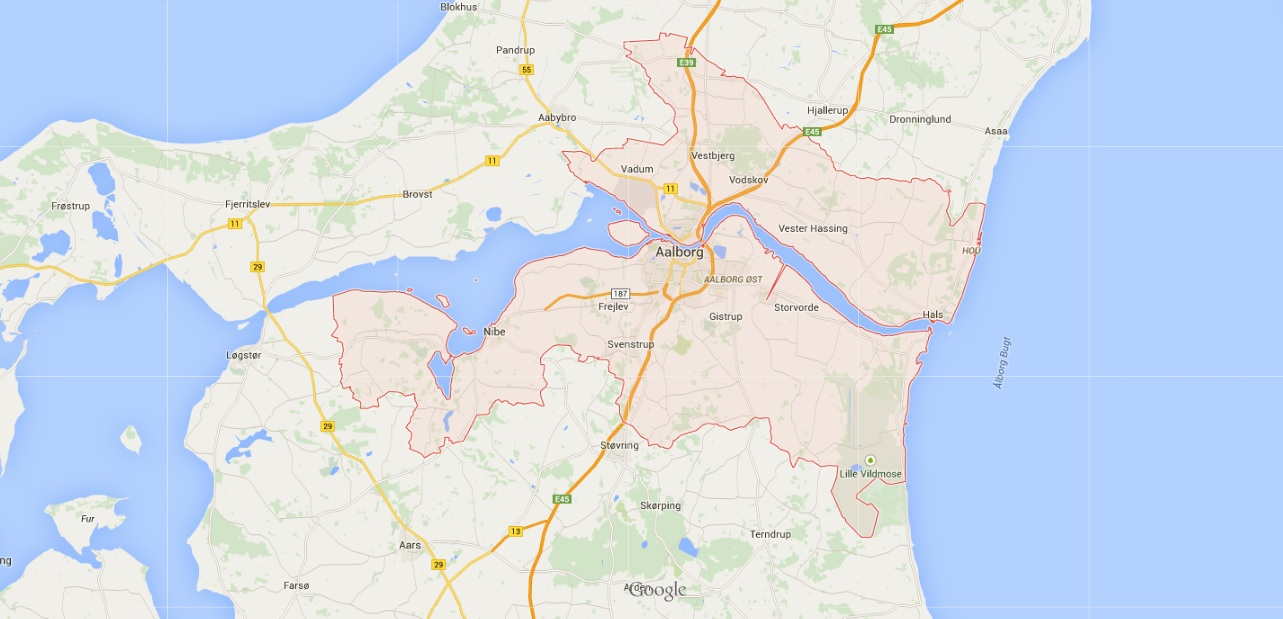
\includegraphics[width=1.0\textwidth]{billeder/aalborgkommune.png}
		\caption{Aalborg Kommune}
		\label{fig:aalborgkommune}
	\end{minipage}\hfill
	\begin{minipage}[b]{0.48\textwidth}\centering
		\centering
		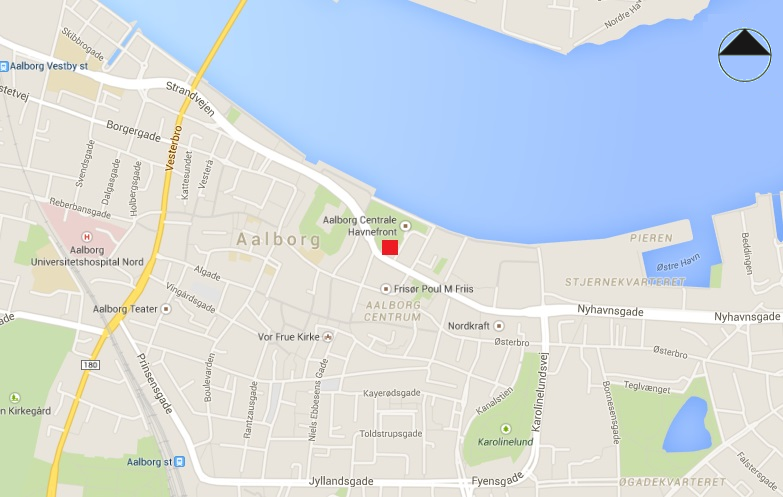
\includegraphics[width=1.0\textwidth]{billeder/aalborg.png}
		\caption{Strøybergs Palæs beliggenhed}
		\label{fig:aalborg}
	\end{minipage}
\end{figure}
\chapter{Problemformulering}

\section{Problemformulering og problemstillinger}
For at gennemføre planen om en tilbygning til Strøybergs Palæ kræves det, at lokalplanen for området stemmer overens med kommuneplanen. Ved konstruktionen af tilbygningen er det også nødvendigt at kende til geologien for området, for at bestemme hvilken type fundering, der skal benyttes. Dertil skal der anvendes en passende ståltype til dimensionering af stålprofilerne, for at tilbygningen har en tilstrækkelig bæreevne. Desuden skal der bestemmes en funderingstype til tilbygningen ud fra områdets geologi og jordbundsforhold. 

\begin{itemize} 
	\item Har Vækstaksen en betydning for tilbygningen af Strøybergs Palæ?
	\item Hvilken ståltype og stålprofil skal der anvendes ved tilbygningen til Strøybergs Palæ? 
	\item Hvilken funderingstype skal der benyttes ved området omkring Strøybergs Palæ? 
\end{itemize} 

\section{Problemafgrænsning}
Dette projekt beskriver tilbygningen af Strøybergs Palæ ud fra både et kontekstuelt og teknisk aspekt. I den kontekstuelle del lægges der vægt på beskrivelsen af Aalborg Kommuneplan samt udviklingen af områderne inden for Vækstaksen; hertil i særdeleshed området omkring havnefronten og Strøybergs Palæ, hvor Vækstaksens betydning for tilbygningen, samt tilbygningen relevans, diskuteres. Dertil beskrives og analyseres lokalplanen for området omkring Strøybergs Palæ, Lokalplan 1-1-107.
\newline \indent{     }  Den tekniske del belyser tilbygningen af Strøybergs Palæ ud fra to emner; konstruktionen af tilbygningen samt de geologiske forhold for området. I konstruktionsdelen opstilles der et statisk system for tilbygningen, som derefter dimensioneres for en række laster. 
\newline \indent{     }  Hertil beskrives de geologiske forhold, som gør sig gældende for Aalborg, hvortil der er foretaget jordbundsanalyser, for at finde frem til, hvilken type fundering der skal benyttes for tilbygningen.  
\chapter{Aalborg i vækst}

\section{Aalborg gennem tiden}
Aalborg er en by fra omkring år 1040, og er i dag Danmarks fjerde største by. Byen har gennem årene udviklet sig til en købstadsby og handelscentrum for Nordjylland. Dette grundet dens beliggenhed ved Limfjordens smalleste punkt og udmundingen af tre større åer, der var grundlag for små havne. Beliggenheden har gjort det muligt for Aalborg, at udvikle sig i størrelse og som by. I 1500-tallet nød byen godt af silde- og korneksport til Norge, samt studeeksport til Tyskland. Da Limfjorden var sandet til, skulle alt eksport vest for Aalborg gå gennem Aalborg for at blive fragtet til Norge og andre steder. Aalborg fik velstand og flere indbyggere der i 1600-tallet nåede op på omkring 4.000 indbyggere. På daværende tidspunkt blev Aalborg Danmarks andenstørste by. Dette varede ikke ved, da andre jyske byer blev prioriteret højere af kongen, og derved udviklede de sig mere eksponentielt i det kommende århundrede end Aalborg. Det, at Limfjorden brød igennem på vestsiden og Danmark mistede Norge, gavnede heller ikke Aalborgs position i forhold til handlen.
\newline \indent{     }  Til trods for dette fortsatte Aalborg alligevel med at udvikle sig, og 1800-tallets industrialisering fik indbyggertallet til at stige stødt. Fra 1830’erne flyttede flere industrier til Aalborg, heriblandt spritfabrikken (forløberen for De Danske Spritfabrikker) og C.W Obels Tobaksfabrik. De store kridt- og lerfund i undergrunden ved Aalborg lagde grunden for cementindustrien, hvor Aalborg Portland, som den største cementfabrik, alene beskæftigede 450 ansatte. Mange flere industrier blev grundlagt eller flyttede til Aalborg, og en del af disse var blandt landets største inden for deres område. Dette fik indbyggertallet til at stige gennem en cirka 50-årig periode til 30.000. Det var ikke kun indbyggertallet der steg. For at Aalborg by skulle kunne følge med eksporten, som også dengang hovedsageligt foregik via skibsfragt, udvidede byen havnen, som i starten af 1900-tallet blev Danmarks næststørste havn \citep{byhistorie}.
\newline \indent{     }  Befolkningstallet er siden 1990'erne vokset, og er i dag stadig stigende \citep{indbyggertal}. Dette er resultatet af, at Aalborg har udviklet sig fra at være en industriby til at være en kompetenceby. Hovedårsagen til denne udvikling er, at størstedelen af industrien, som Aalborg var kendt for at have inde i centrum af byen, og som var hoveddelen af identiteten af Aalborg, er flyttet til yderkanterne af byen. I stedet er der nu fokus på at have et levende Aalborg, som skal kendes for at være en kompetenceby.
\newline \indent{     }  Havnefronten på Aalborgs side af Limfjorden er blevet et nøglepunkt for Aalborg Kommune, da denne tidligere var fyldt med fabrikker. Der er siden år 2000 foretaget mange ændringer ved havnefronten for at gøre Aalborg mere attraktiv og give den en ny identitet som byen for kompetence og innovation \citep{brughavnen}.
\newline \indent{     }  Disse ændringer har blandt andet været, at dele af den industri, som lå ved havnefronten, er flyttet ud af det centrale Aalborg og ud til mere fremkommelige steder. Dette har givet plads til et område med mere serviceerhverv. Denne type erhvervsområde gør det også muligt at opføre boliger i området, da der ikke vil være de samme støjgener, som der ville komme fra et industriområde. Denne udvikling fik muligheden for at tage fart, efter der blev lavet en ændring i planloven den 1. juli 2003, der ændrede bestemmelserne for byomdannelse. Denne ændring gjorde det muligt for kommunerne at omdanne tidligere industriområder til blandt andet servicebygninger og boligområder \citep{sort}.
En del af denne udvikling har været bebyggelsen af flere forskellige kollegieboliger som for eksempel Bikuberne ved Utzon Parken og Larsen Waterfront. Disse boliger ligger tæt op ad nogle nye kulturelle bygninger som Utzon Centeret og Musikkens Hus, samt Nordkraft, som tidligere var et kulkraftværk, men i dag er omdannet til et kulturhus med mulighed for både sport og kulturelle oplevelser. Disse byggerier viser den udvikling, som Aalborgs centrale havnefront gennemgår fra industriområde til boligområde. Havnefronten er i en stadig udvikling, da der fortsat kommer flere boligbyggerier til. Det har også givet anledning til tilbygninger, her i blandt en kommende tilbygning til den bevaringsværdige bygning Strøybergs Palæ, der ligger ved havnefronten \citep{havnefronterne}.

\section{Strøybergs Palæ}
Strøybergs Palæ er en ejendom fra år 1908, beliggende centralt i Aalborg ved havnefronten, Utzon Centret, butikscentret Friis og Slotspladsen.
\newline \indent{     }  Lokalplan 1-1-107 har opdelt området, omfattende Strøybergs Palæ, i to delområder. Delområde A med matrikelnummer 518g omfatter den bevaringsværdige hovedbygning til Strøybergs Palæ, og delområde B med matrikelnummer 519b omfatter den bevaringsværdige sidebygning til Strøybergs Palæ (\citep{lokalplan}, s. 7). Hovedbygningen ligger på Nyhavnsgade 11, og er fordelt på stueetage, 1. sal, 2. sal samt kælder og tagetage, mens sidebygningen ligger på Nyhavnsgade 9 og er fordelt på stueetage, 1. sal, 2. sal og 3. sal samt kælder og tagetage. Ejendommen er op til 22 m høj og har et samlede grundareal på 1037 kvm \citep{byggesagen}.
\newline 
\newline 
Strøybergs Palæ er siden opførelsen blevet anvendt til mange forskellige formål. 
\newline \indent{     }  Nyhavnsgade 9 blev opført som en ejerlejlighedsejendom, opdelt i ni ejerlejligheder af forskellig størrelse, og Nyhavnsgade 11 blev på daværende tidspunkt primært brugt til erhverv. 
\newline \indent{     }  Kælderen blev i år 1920 omdannet fra hestestald til garage, og er derudover blevet brugt som lager.
\newline \indent{     }  I dag bliver Strøybergs Palæ hovedsageligt anvendt til erhverv, og huser blandt andet ejendomsmæglerfirmaet EDC Danebo.
\newline \indent{     }  Siden år 2010 har det været på tale, at lave en tilbygning til Strøybergs Palæ, og omdanne bygningen til lejligheder med udsigt over Limfjorden \citep{link}. I den forbindelse blev lokalplan 1-1-107 udarbejdet med et ønske om at lave denne tilbygning. Området ønskes hovedsageligt anvendt til kontor- og serviceerhverv samt boligformål (\citep{lokalplan}, s. 7).
\chapter{Et fremtidigt Aalborg}
Nedenstående afsnit vil behandle Aalborgs kommuneplan med primært fokus på Aalborgs Vækstakse, der er ét af fem hovedpunkter i kommuneplanen. En beskrivelse af de fire resterende fokuspunkter vil give en forståelse for, at kommunen til dels har flere tanker om byens udvikling, og alle fem fokuspunkter har relevans for hinanden og gavner til byens udvikling.

\section{Kommuneplan}
En kommuneplan er kommunens overordnede plan for kommunens udvikling. Indenfor en periode på 12 år fastlægger kommunen de overordnede mål og retningslinjer for kommunens udvikling såvel i byerne som i det åbne land \citep{kommuneplan1}. 
\newline
\newline
En kommuneplan består af; en hovedstruktur, retningslinjer, kommuneplanrammer, bilag og tilhørende planredegørelse. 
\newline \indent{     }  Hovedstrukturen er den overordnede, strategiske og sammenfattende fysiske plan for kommunen. Den fastlægger de overordnede mål for udviklingen inden for de enkelte sektorer for hele kommunen og for de enkelte områder \citep{kommuneplan1}.
\newline \indent{     }  Retningslinjerne udgør de overordnede rammer for kommuneplanlægningen. De fastsætter principperne for arealanvendelsen i kommunen, og danner ligeledes grundlag for kommunens administration af planlovens landzonebestemmelser, samt administrationen af kompetencer indenfor anden lovgivning, herunder natur-, miljø-, bygge- og vejlovgivningen og husdyrloven. Retningslinjerne angiver sammen med områdeudpegningerne hvilke forhold, der skal tages hensyn til i administrationen, og hvilke konkrete skøn der skal foretages for disse områder \citep{retningslinjer}. 
\newline \indent{     }  Kommuneplanrammerne styrer den overordnede arealanvendelse og danner ramme for indholdet i nye lokalplaner. Planrammerne fastlægger dermed mål, muligheder og begrænsninger for arealanvendelse i de enkelte dele af kommunen. Kommuneplanrammerne har to niveauer: 1) by/bydel/landområde og 2) rammeområder. Det første niveau “by/bydel/landområde”, behandler områdets særlige problemer, værdier og muligheder i en sammenhæng. Det andet niveau “rammeområder”, er det mest detaljerede niveau i kommuneplanen rent geografisk. Her fastsættes de bestemmelser, der danner grundlag for lokalplaner \citep{rammer}. 
\newline \indent{     }  Bilag er de generelle rammebestemmelser, hvor der henvises til de aktuelle bilag fra de enkelte emner \citep{bilag}.
\newline \indent{     }  Planredegørelser beskriver forudsætninger for, og ændringerne i den konkrete planlægning. Byrådet offentliggør, sammen med alle kommuneplanforslag eller med forslag til kommuneplantillæg\footnote{Opstår der problemer med at realisere en lokalplan ud fra kommuneplanen, så anvendes der et kommuneplantillæg, som er et supplement til den eksisterende kommuneplan. Denne kan justere og ændre bestemmelserne i kommuneplanen, for at gøre det muligt at realisere lokalplanen \citep{kommuneplan2009}.}, en redegørelse om planens baggrund og sammenhæng med anden planlægning. Kommuneplanen ledsages også af en planredegørelse og planstrategi, hvilken laves minimum hvert fjerde år i tilknytning til kommunens budget. Denne er byrådets instrument og baner vejen for at realisere kommuneplanens mål. Her oplyses blandt andet om kommuneplanens væsentlige forudsætninger, planlægninger der er gennemført det forgangne år, det kommende års kommuneplaninitiativer samt byrådets vurdering af og strategi for udviklingen for både det kommende år (budgetåret), de kommende fire år (overslagsårene) og en længere periode på 12 år. Desuden laves der jævnligt statusredegørelser, som giver et overordnet billede af kommunens fysiske udvikling og præsenterer de økonomiske tiltag, der knytter sig til kommunens sektorer og geografiske områder \citep{planredegorelse}.

\section{Aalborg Kommuneplan}
Aalborg Kommuneplan beskriver kommunens udvikling inden for de 12 kommende år og er opdelt i fem fokuspunkter: 
\begin{enumerate}
\item Byerne - et godt sted at bo hele livet
\item Nødvendige forbindelser - mobilitet
\item Det åbne land
\item Bæredygtighedsprofil
\item Aalborg - den attraktive storby
\end{enumerate}
Et af Aalborg Kommuneplans fem fokuspunkter er “Byerne - et godt sted at bo hele livet”. De større byer under Aalborg Kommune har, i kraft af nærheden til Aalborg, en god infrastruktur,  et varieret serviceudbud samt tilstrækkeligt befolkningsunderlag. Det er et særligt potentiale for byvækst, der skal udnyttes for at understøtte Aalborg som Norddanmarks Vækstdynamo. 
\newline \indent{     }  Byvæksten skal have særligt fokus på nye, kreative boligformer, som tilgodeser klimaudfordringer, demografiske udfordringer og bæredygtighed. 
\newline \indent{     }  Ikke kun de større byer nær Aalborg har en væsentlig rolle i projektet. Mindre byer og landsbyer er også i fokus, og har en særlig rolle som opland til Aalborg med store kvaliteter indenfor bosætning, rekreation og friluftsliv \citep{byerne}.
\newline
\newline
Et andet af Aalborg Kommuneplans fem fokuspunkter er “Nødvendige forbindelser - mobilitet”. Dette fokuspunkt omhandler byens behov for forbindelser, der kan håndtere transportbehovet og gøre det mere attraktivt at benytte offentlig transport såsom bus og tog, samt at tage cyklen, da  Aalborg Kommune har en målsætning om at blive Danmarks førende cykelby. Kommunens mål er færre bilkøer, god adgang til indkøb, service og arbejdspladser samt sikring af forbindelser, der understøtter en effektiv godstransport. Derudover satser Aalborg på en letbane som det bærende element i byen \citep{mobilitet}.
\newline
\newline
Fokuspunktet “Det åbne land” omhandler benyttelsen og beskyttelsen af det åbne land. Dette skal ske på et bæredygtigt grundlag med plads til oplevelser, natur, erhvervsinteresser og vedvarende energi. Det åbne land skal danne ramme om levende og aktive områder \citep{land}.
\newline
\newline
Aalborg Kommune har også stor fokus på bæredygtighed og har dertil punktet “Bæredygtighedsprofil”. Udviklingen af et bæredygtigt samfund omhandler flere punkter, såsom at passe på miljøet, klimaet og naturen, om at bygge byer for mennesker og om at få det bedste ud af den nuværende økonomiske virkelighed. En bred tilgang til bæredygtighed er derfor udgangspunktet \citep{profil}.

\subsection{Aalborg Vækstakse}
Det femte og sidste fokuspunkt i Aalborgs kommuneplan er “Aalborg - den attraktive storby”. Dette fokuspunkt indeholder yderligere tre punkter; vækstaksen som byens motor, byudviklingsprincipper for Aalborg og fokus på bykvalitet. 
\newline
\newline
Aalborg Kommune har valgt at koncentrere sig om et vækstbånd, kaldet Vækstaksen, som skal danne grundlag for Aalborgs udvikling, hvor der er fokus på det generelle udviklingsprincip \citep{kommuneplan3}. Området går fra Aalborg Lufthavn i vest, gennem midtbyen, til Campus og videre ud til østhavnen, hvilket illustreres på Figur \ref{fig:vaekstakse}. 
\newline \indent{     }  Blandt Vækstaksens mest centrale elementer er færdiggørelsen og videreudviklingen af en række større områder i Aalborg, som for fremtiden skal være med til at skabe Aalborg som storby og præge dens identitet. Gennem disse færdiggørelser vil bykvaliteten øges, og byen vil blive mere attraktiv. Der lægges derfor stor vægt på arkitektoniske overvejelser samt historiske skulpturer og monumenter, når der skal bygges og renoveres \citep{kommuneplan3}. 
\newline \indent{     }  Her har havnefronten, som et af de første områder, gennemgået en stor renovering, hvor der er etableret både Aalborg Havnebad, Jomfru Ane Parken og sportsfaciliteter. Derudover blev Tivoli Karolinelund fjernet i 2011, og i 2012 åbnede en ny Karolinelund park, som nu danner ramme for mange forskellige nichekulturer, såsom koncerter, Platform 4, legepladser og meget mere, og parken er fortsat under udvikling \citep{jomfruaneparken} \citep{karolinelund}. 
\newline \indent{     }  Aalborg er gennem renoveringen af den nye havnefront også vokset som kulturby, og i dag er kultur blevet en bærende del af byen, hvor der findes KUNSTEN Museum, Aalborg Kongres \& Kultur Center, Nordkraft samt det nye Musikkens Hus, der åbnede i 2014, hvor der hver uge afholdes forskellige koncerter og andre arrangementer. Dette er altsammen med til at styrke Aalborg som vækstby og byens erhvervsturisme \citep{kommuneplan3}. Ligeledes er der planer om en ny kulturbro på Jernbanebroen, som også skal være med til at styrke kulturen i Aalborg og Aalborg Kommune. Ved at styrke kulturen styrkes bykvaliteten også, og byen bliver en levende by, hvor det er muligt at binde shopping, café og kulturliv sammen \citep{kulturbro} \citep{musikkenshus}.
\newline \indent{     }  Den gamle Eternitgrund i Aalborg havde i en lang årrække stået ubrugt hen, men gennem de sidste fem år er der etableret både studieboliger, supermarkeder, fitnesscenter og et nyt legeland for børn. Virksomheder som Plus Bolig og COWI er ligeledes flyttet ned på Eternitten, og i dag er Eternitten blevet en stor drivkraft for Aalborg,  hvor der fortsat  er fremtidige planer om grønne arealer også \citep{eternitten}.
\newline \indent{     }  Projektet om Vækstaksen er i fuld gang, og inden for den nærmeste fremtid skal også Godsbanearealet og det østlige Aalborg udvikles, for at øge oplevelsesmulighederne, kulturtilbudene og skabe attraktive og bæredygtige livsvilkår her. Det er dog ikke kun nybyggerier, som Vækstaksen har fokus på. For Aalborg Kommune er det også vigtigt, at vedligeholde de gamle bygninger, for at opretholde byens historisk identitet \citep{kommuneplan3}.

\begin{figure}[htbp]
	\centering
	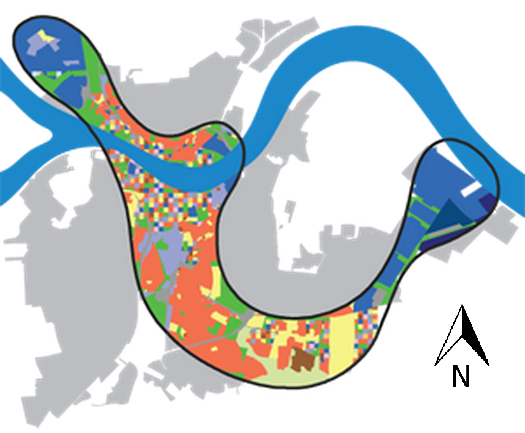
\includegraphics[width=0.5\textwidth]{billeder/vaekstaksen.png}
	\caption{Aalborgs Væsktakse}
	\label{fig:vaekstakse}
\end{figure}

Vækstaksen skal være attraktiv for alle aldersgrupper og skal derfor have noget at tilbyde hver enkelte borger, og skal ligeledes være med til at skabe oplevelsesmuligheder og kulturtilbud.
\newline \indent{     }  En stor del af planerne for Vækstaksen er byfortætning, mobilitet, studieby og miljø \citep{kommuneplan3}. 
Der er i Aalborg Kommune stor udviklingspotentiale inden for byfortætning. På Figur \ref{fig:udvikling} ses udviklingspotentialet i Vækstaksen. De markerede lilla områder er der hvor Aalborg Kommune har bedst udviklingspotentiale \citep{kommuneplan3}.
\newline \indent{     }  Dette udviklingspotentiale er i form af tilbyggelse og omdannelse af boliger, arbejdspladser og naturområder. Byfortætning kan resultere i en meget presset infrastruktur, derfor er mobilitet et essentielt punkt for optimering af byens potentiale \citep{kommuneplan3}. Det er vigtigt, at der er let og hurtigt adgang til offentlig transport, og det skal gøres mere attraktivt, at tage cyklen. Målet er, at få en stor by til at opfattes som en “lille by”, ved at gøre transport lettilgængeligt og derfor nemt at komme fra bydel til bydel. Infrastrukturen vil styrkes blandt andet via en cykelmotorvej samt en kommende letbane, som skal forbinde Østhavnen, Campus, det kommende superhospital i Aalborg Øst, midtbyen og ud til Aalborg Lufthavn \citep{kommuneplan3}.

\begin{figure}[htbp]
	\centering
	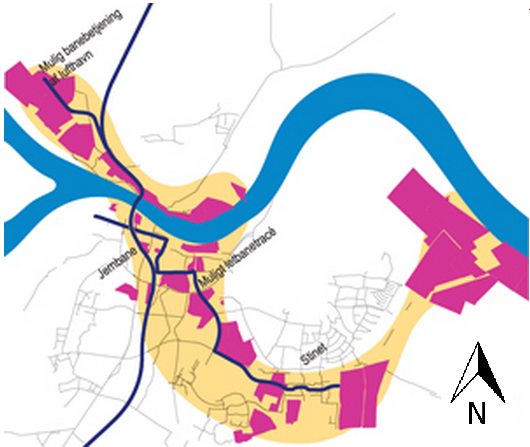
\includegraphics[width=0.5\textwidth]{billeder/udvikling.png}
	\caption{Udviklingspotentiale}
	\label{fig:udvikling}
\end{figure}

Ved Vækstaksens to endepunkter ligger Aalborgs største industriområder, Aalborg Østhavn og Aalborg Lufthavn. Disse industriområder er kommet til, efter industrifirmaer er begyndt at flytte fra havnefronten og ud til yderkanten af Vækstaksen. Trods denne flytning forbliver Aalborg en erhvervsby samtidig med, at den gradvist omdannes til en studieby. De store industrifirmaer er stadig vigtige for Aalborg, da de er med til at skabe omsætning og arbejdspladser \citep{kommuneplan3}. 
\newline \indent{     }  Da Aalborg gradvist omdannes til en studieby, er det vigtigt, at der i Vækstaksen støttes op om Aalborgs studieliv og studiemiljø, da 10\% af Aalborg Kommunes befolkning består af studerende \citep{campus}. Et godt studiemiljø vil styrke innovation, konkurrence og vækst i erhvervslivet. Det er nødvendigt med gode uddannelsesmuligheder, faciliteter samt ungdomsboliger til de studerende, hvilket også vil gøre det attraktivt for udefrakommende at studere i Aalborg. Centrum for studielivet i Aalborg udspringer fra Campus i Aalborg Øst, hvor størstedelen af de videregående uddannelser findes \citep{kommuneplan3}. 
\newline
\newline
Aalborg Kommune ønsker også at udvikle byens natur og udendørsliv. Til at opnå dette vil kommunen opføre parker, stisystemer og vandløb. Vandløbene vil give byen historisk identitet, samtidig med at de vil beskytte byen under eventuel øget vandstand, da de kan forsinke vandet \citep{kommuneplan3}. Formålet med parkerne og et naturrigt Aalborg er at skabe et sundhedsfremmende forhold for alle aldersgrupper og beskytte klimaet. Desuden vil Aalborg Kommune gøre Aalborg til en miljøvenlig storby, som antages at gøre byen mere attraktiv, og dermed øge indbyggertallet. Derfor vil Aalborg Kommune genoprette naturen og give velfærd til byens borgere \citep{kommuneplan3}.

\section{Vækstaksens betydning}
 Formålet med Vækstaksen er, at styrke Aalborg som by, og der er en forventning fra Aalborg Kommune om, at byen bliver Nordjyllands Vækstdynamo, men er dette realistisk? Nedenstående afsnit vil stille spørgsmålstegn ved Vækstaksen, og diskutere, hvilken sammenhæng Strøybergs Palæ og Vækstaksen har med hinanden. I den forbindelse vil der diskuteres, hvorfor der ønskes en tilbygning, og hvorfor det netop er i dette område, det er fordelagtigt at udvide.

\subsection{Er Vækstaksen realiserbar?}
Vækstaksen er placeret således, at den går gennem Aalborgs centrale områder for kultur, uddannelse, erhverv og miljø.  Aalborg Kommune ønsker at etablere en god infrastruktur, som den kommende Letbane for eksempel skal hjælpe med \citep{kommuneplan3}. Det er fordelagtigt at udvide samt udvikle i Vækstaksen, da områderne samt virksomhederne er drivkraften for Aalborg \citep{bedreoverblik}, og det er her, at byens liv er, og fremtiden skal skabes. Selvom områderne i dag fungerer som drivkraft, skal disse stadig videreudvikles, da Aalborg er en by i stor vækst, hvilket afspejles af både stigende indbyggertal og antal virksomheder, som flytter til og skabes i Aalborg \citep{statistik}\citep{virksomheder}. Derfor kan Aalborg Kommune ikke blot stille sig tilfreds med de nuværende tilstande, da byen skal udvides, for at være forberedt på fremtiden; ellers er der ikke plads til udviklingen, og den vil bremses, gå helt i stå eller i værste fald gå den anden vej.
\newline \indent{     }  Udviklingen af byen vil primært ske gennem en byfortætning, da de centrale områder allerede i dag er fyldt med liv samt kultur, erhverv og uddannelse. Der er altså ikke tale om store udvidelser af områderne, men snarere optimeringer af de allerede eksisterende områder, og derfor kan infrastrukturen opleve problemer. 
\newline \indent{     }  I takt med at indbyggertallet stiger kan det formodes at antallet af biler vil stige. Derfor kan spørgsmålet stilles, om det er realistisk med en fortætning af byen samtidig med, at Aalborg Kommune har en målsætning om, at det skal være let at færdes i byen som fodgænger, cyklist og med offentlig transport \citep{kommuneplan3}. Dette afspejler sig i trafikken omkring Nyhavnsgade, som strækker sig fra Nordkraft forbi Strøybergs Palæ og videre langs med havnefronten. Her er vejen ændret fra en 4-sporet vej til en 2-sporet. Derfor er antallet af bilister næsten halveret, fra 20.500 (ÅDT) til 11.000 (ÅDT), og hastigheden er sænket (\citep{lokalplan}, s. 6). Selvom Aalborg Kommune har sænket antallet af bilister omkring centrum, så vil en udvikling af byen og et øget indbyggertal betyde, at flere bilister igen vil køre gennem centrum, så trafikken igen vil begynde at stige. Derfor har Aalborg Kommune kun løst problemet delvist, for med tanke på en kommende vækst for byen så øges årsdøgntrafikken. Det betyder, at Aalborg Kommune igen vil stå med et problem, hvis ønsket om at opretholde et lavt antal bilister samt at det skal være let at færdes i byen for de bløde trafikanter, skal imødekommes. Nu er det blot ikke muligt at skære ned på antallet af kørespor, og derved skal der findes en ny løsning, med mindre Aalborg Kommune ændrer synspunkt på problemet.
\newline \indent{     }  Aalborg Kommune ønsker færre biler omkring centrum, for at gøre det mere attraktivt og lettere for de bløde trafikanter at færdes \citep{aalborgletbane}\citep{nordjyske}. Letbanen vil gøre det mere attraktivt at undvære bil i Aalborg, men i takt med fortætningen er spørgsmålet, om det er nok, til at det føles let at færdes i Aalborg. Et andet fokuspunkt er en tredje Limfjordsforbindelse, som der i dag er ønske om \citep{limfjordsforbindelsen}. Trafikken i morgen- og eftermiddagstimerne til og fra Aalborg er tæt, og særligt når der opstår et trafikuheld i en af Limfjordsforbindelserne for køretøjer over Limfjorden, så opstår der trafikale problemer omkring den anden forbindelse, og centrum bliver overbelastet. Dette kan en tredje Limfjordsforbindelse afhjælpe, da den af naturlige årsager vil medføre flere biler på vejen, og omvendt vil trafikken også blive mere jævn fordelt, da der kommer en ekstra strækning, som bilisterne kan anvende. Dette kan gavne Aalborg Centrum, både ved den daglige trafik omkring centrum, og ved et eventuelt uheld i Limfjordstunnelen, da det ikke længere kun vil være centrum, der så giver adgang for bilister til at passere over på den anden side af fjorden. Her vil en tredje forbindelse så også vil kunne anvendes, og dermed lette trafikken. 
\newline
\newline
Aalborg har et ønske om at være Danmarks bedste studieby \citep{ungdom}, og derfor kræves der nok studieboliger til de studerende. Der er i landet en generel mangel på studieboliger, og dette gør sig også gældende for Aalborg, selvom det ikke er i ligeså høj grad som eksempelvis København. Det skyldes Aalborgs store fokus på de studerende og behovet for studieboliger, hvoraf der er blevet bygget over 6.000 studieboliger siden 2010 inden for Vækstaksen, både på Aalborg og Nørresundby siden, og der bygges fortsat flere nye boliger i dag \citep{studieboliger}. Dette er et led i Vækstaksen og planerne om Aalborgs fremtid, hvilket indtil videre er godt realiseret. De seneste fem år har de videregående uddannelser oplevet rekordmange ansøgninger og dermed flere studerende \citep{uddannelser}, hvilket betyder, at studieboligerne hurtigt bliver lejet ud. Der er fra år 2009 til 2014 kommet ca. 8.000 flere studerende til (\citep{unital}, s. 9). Et af kommunens fokuspunkterne er, at gøre Aalborg en attraktiv studieby med studievenlige priser på boligerne. Sammenlignes priserne med de tre andre storbyer i Danmark; Aarhus, Odense og København, er boligerne i Aalborg væsentlig billigere \citep{home}, hvilket kan være en medvirkende faktor til, at Aalborg er attraktiv for de unge. Dette punkt fra Vækstaksen er derfor godt på vej til at blive realiseret.
\newline
\newline
Aalborg Kommune har også et ønske om, at byen skal være for alle mennesker i alle aldersgrupper samt et attraktivt sted for erhverv \citep{kl}\citep{kommuneplan3}. Spørgsmålet er dog, hvor erhverv skal etableres inden for Vækstaksen, og hvad der kan gøres for de indbyggere, som ikke er studerende. Havnefronten, som er en af de bærende elementer i Vækstaksen, anvendes ikke kun af unge, men også af børnefamilier. Derudover byder Aalborg også på naturområder og attraktioner, som er for alle i alle aldersgrupper.
\newline
\newline
For nye virksomheder gælder det, at der skal være kontorlokaler og bygninger, som kan huse virksomhederne. Ligeledes skal virksomhedens beskæftigelse gerne passe med Aalborg, således at der er en sammenhæng mellem kunde og virksomhed. Med en målsætning om, at være en attraktiv storby med mange muligheder for virksomheder, er der derfor et godt grundlag for at drive virksomhed i Aalborg, også i fremtiden. Indenfor Vækstaksen ligger der utallige virksomheder, men der er stadig tomme erhvervslokaler, som vil give plads til flere virksomheder. Heriblandt skal der ske en udvidelse af Strøybergs Palæ, som har en central beliggenhed i Vækstaksen, helt nede ved havnefronten.


\subsection{Hvorfor udvide Strøybergs Palæ?}
Strøybergs Palæ ligger i Vækstaksen. På Figur \ref{fig:udvikling} ses det, at Strøybergs Palæ ligger i det lilla område og er dermed i et område, hvor der er størst mulighed for udvikling inden for Vækstaksen. Grundet havnefrontens udvikling de sidste 10 år, har der været fokus på udviklingen her, og nu har Aalborg Kommune godkendt forespørgslen om en tilbygning til Strøybergs Palæ, da der allerede er bygget Musikkens Hus, havnefronten, Utzon Centeret og Utzon Parken omkring området. Udviklingen omkring havnefronten er sket i takt med Vækstaksens fokus herpå. Om havnefronten havde fået en udvikling overhovedet eller i lige så høj grad, hvis tankerne og ideérne omkring Vækstaksen ikke var blevet sat i værk, kan diskuteres. Uden en vækstakse vil der stadig ske en udvikling ved havnefronten, men ikke i ligeså høj grad, som nu, hvor Vækstaksen bringer ekstra fokus på området. Dog må det formodes, at havnefronten ikke vil udvikle sig i samme retning i forhold til de kulturmæssige fokuspunkter som Vækstaksen giver. 
\newline \indent{     }  Det kan ligeledes diskuteres om Vækstaksen overhovedet har haft indflydelse på udvidelsen af Strøybergs Palæ. Placeringen af Strøybergs Palæ midt i Vækstaksen, kan tænkes at have haft indflydelse på beslutningen om, at der skal laves en tilbygning, fordi bygningen skal leve op til Aalborg Kommunes forventninger, og ønsker for fremtiden. Tilbygningen kan bruges til erhvervslokaler, og dette vil kunne tiltrække en eller flere nye virksomheder til området, og dermed være med til at udvikle både området og Aalborg by. Omvendt kan spørgsmålet dog også stilles, om denne tilbygning vil få den ønskede effekt og kunne leve op til disse målsætninger. Det vil være naivt at tro, at en udvidelse på nogle få hundrede kvadratmeter vil gøre en betydende forskel for Aalborg, og det kan derfor ikke alene være grunden til tilbygningen, men snarere en af flere årsager. Strøybergs Palæ er kun en lille del af Vækstaksen, og skal derfor ikke bære Aalborgs udvikling og vækst alene.
\newline \indent{     }  Hovedpunkterne i Vækstaksen er, at Aalborg skal vokse som by, og udvikles gennem en byfortætning, hvor målet er, at tiltrække flere  virksomheder og indbyggere. En udvidelse af Strøybergs Palæ vil give ekstra erhvervslokaler og/eller lejligheder, og dette passer godt sammen med Vækstaksen. Tilbygningen betyder desuden, at Strøybergs Palæ vil få et mere harmonisk udseende ud mod vandet, da tilbygningen vil blive bygget i samme arkitektoniske stil som resten af bygningen, og den nordøstlige del af bygningen vil komme op i cirka samme højde, som resten af bygningen. Sammen med resten af havnefronten vil Strøybergs Palæ gennemgå en renovering, som løfter udseendet samt medfører, at området vil få en mere ensformet og harmonisk stil.
\newline \indent{     }  Det, at området bliver et centralt fokuspunkt for fremtiden betyder også, at området bliver mere attraktivt, idét der kommer til at ske en fortsat udvikling af området, og netop derfor kan en tilbygning være en god investering, da det giver ekstra plads og bedre forudsætninger for udviklingen.
\chapter{Udvikling af området}
I det følgende afsnit vil lokalplanen for området ved Strøybergs Palæ beskrives, da denne sammen med kommuneplanen indeholder en række informationer om Strøybergs Palæ, og fastsætter rammerne for den kommende tilbygning. 
\newline \indent{     }   Til sidst vil der foretages en sammenligning mellem den førhen gældende lokalplan for området og den nuværende lokalplan, for at undersøge, hvilke ændringer der har været nødvendige at foretage, for at kunne realisere tilbygningen til Strøybergs Palæ.

\section{Lokalplan}
En lokalplan tager udgangspunkt i en fremsat kommuneplan, og har til formål at styre udviklingen i et område. Lokalplanen skal give borgerne og byrådet et indblik i et bestemt område og give dem mulighed for at komme med tiltag til den fremlagte plan. Her fastsætter byrådet rammerne for, hvordan arealer, bygninger, beplantning, veje, stier m.fl. skal anlægges i et givent område. Lokalplaner skal ifølge planloven udformes af byrådet, der har pligt til dette, før der kan gennemføres større bygge- og anlægsprojekter \citep[ s. 4]{lokalplan}.
\newline
\newline
En lokalplan indeholder punkterne; redegørelse, planbestemmelser og bilag \citep[ s. 4]{lokalplan}.
\newline \indent{     }  Planen starter med en redegørelse, hvor lokalplanens baggrund og formål fastsættes og hele indholdet fremlægges. Der bliver også redegjort for miljømæssige forhold, hvordan lokalplanen forholder sig til andet byggeri, og om der kræves tilladelser eller anden slags dispensationer fra forskellige myndigheder.  
\newline \indent{     }   I lokalplanen informeres der om planbestemmelser, som er områdets fremtidige anvendelse. Dette illustreres via tekst og billeder.
\newline \indent{     }  Til sidst i lokalplanen ligger alle bilagene. Disse består oftest af forskellige kort (matrikelkort, arealanvendelseskort m.m.) samt forskellige tabeller omkring støj fra erhverv og trafik m.m. Bilagene er med til at uddybe og illustrere lokalplanbestemmelserne.
\newline
\newline
Byrådet kan til enhver tid udarbejde et lokalplanforslag. Når et forslag til lokalplanen er udformet, skal det offentliggøres i mindst otte uger, hvor borgerne kan komme med indsigelser eller forslag til ændringer. Efter de otte ugers offentliggørelse bedømmer byrådet, hvorvidt eventuelle indsigelser eller ændringer vil blive taget op. Dernæst vedtages planen, hvor den bekendtgøres i avisen og er hermed bindende for ejendommene, som ligger i lokalplanområdet.
\newline \indent{     }  Der må ikke laves ændringer i området i strid med lokalplanen, dog må eksisterende bebyggelser og anvendelse, der er etableret før lokalplanforslagets offentliggørelse, fortsætte. Endvidere er der ikke pligt til at gennemføre tiltag, der beskriver lokalplanen \citep[ s. 4]{lokalplan}.

\section{Lokalplan 1-1-107}
Lokalplan 1-1-107 er lokalplanen for området ved Strøybergs Palæ. Lokalplanen er vedtaget af Aalborg Byråd den 12. november 2012, og offentligt bekendtgjort den 21. november 2012 \citep[ s. 20]{lokalplan}.
\newline \indent{     }  Området for lokalplanen er ca. 1.200 $m^2$, og ligger ca. 100 m fra Limfjorden. Øst for lokalplanområdet ligger Gammel Havn, mod nord og vest ligger Utzon Parken og mod syd Nyhavnsgade. Ud over Strøybergs Palæ, der ligger i planområdet, er der også enkelte mindre bygninger, garager m.m. For at lokalplanen kan blive realiseret, skal mindre bygninger nedrives, hvis de ikke er bevaringsværdige \citep[ s. 6]{lokalplan}. Området, som lokalplanen dækker, ses på Figur \ref{fig:1-1-107}.
\newline \indent{     }  Lokalplanen er udarbejdet med et ønske om, at lave en tilbygning til Strøybergs Palæ, hvor anvendelsesmulighederne i området således vil blive ændret til beboelse, serviceerhverv og kontorerhverv. Lokalplanen er udformet således, at den tager hensyn til, at den nye bebyggelse udformes efter den eksisterende bevaringsværdige bygning, eventuelt med et nutidigt arkitektonisk udtryk, således der er harmoni mellem den nuværende bygning og tilbygningen. Her tages der hensyn til bygningsskala, facaderytme og farve, da Strøybergs Palæ er vurderet til at være en bevaringsværdig bygning med en bevaringsværdi 4, som er middelværdi \citep[ s. 5 og 9]{lokalplan}. Bevaringsværdien bestemmes på baggrund af fem værdier; arkitektonisk værdi, kulturhistorisk værdi, miljømæssig værdi, originalitet og tilstand, hvor vurderingen er givet i forhold til helhedsindtrykket af bygningens kvalitet og tilstand, dog vil den arkitektoniske- og den kulturhistoriske værdi veje tungest for bevaringsværdien. Bygninger med bevaringsværdi 2-4 er bygninger, som er fremtrædende grundet deres arkitektur, kulturhistorie og håndværksmæssige udførelse \citep{bevaringsvaerdi}. Lokalplanen fortæller desuden, at tage skal udføres som sadeltage eller som flade tage \citep[ s. 17]{lokalplan}.
\newline \indent{     }  Lokalplanen indeholder to delområder, hvor delområdet B er hovedbygningen af Strøybergs Palæ, mens delområde A er sidebygningen dertil og et byggefelt liggende mod nord, hvilket er illustreret på Figur \ref{fig:aogb}. Inden for delområde A må ny bebyggelse opføres i 4 etager, samt en tagetage, og med en kælder maksimalt 1,25 m over terræn, som kan anvendes til parkering, depot og lignende. Inden for delområde B må ny bebyggelse opføres i 3 etager samt en tagetage og med en kælder maksimalt 2 m over terræn. I alt må tilbygningen højst være 19 m høj \citep[ s. 7 og 16]{lokalplan}.

\begin{figure}[htbp]
	\centering
	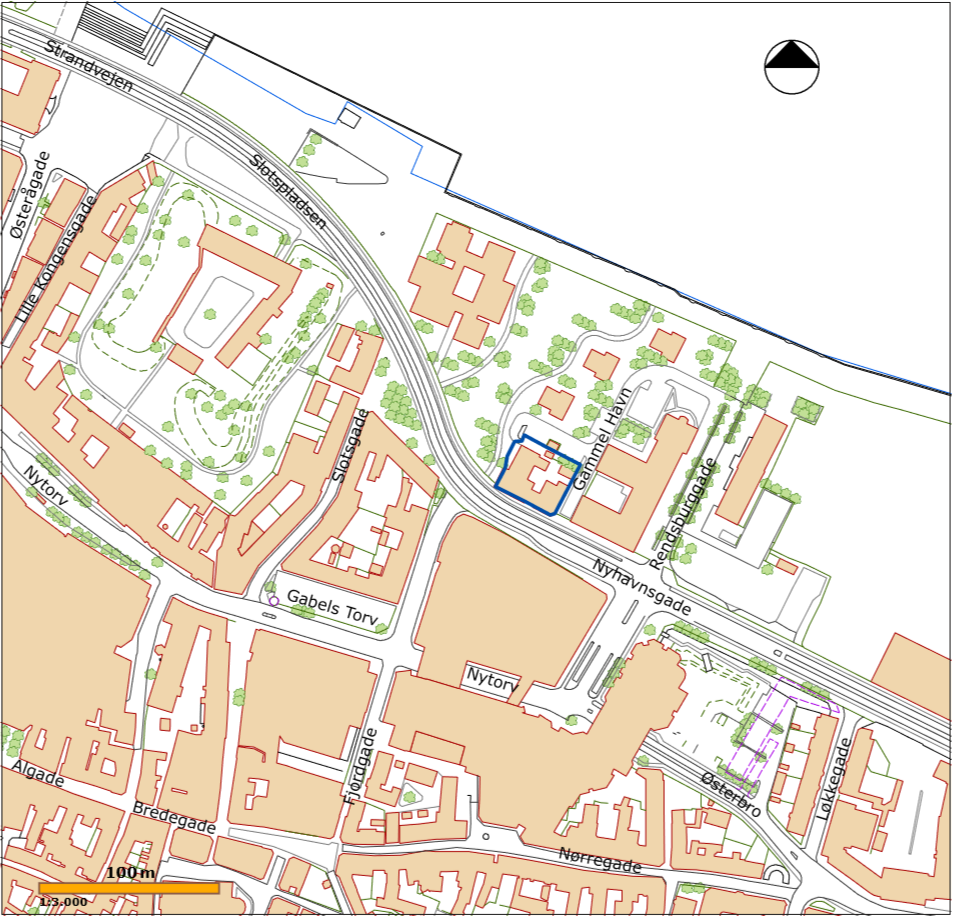
\includegraphics[width=0.7\textwidth]{billeder/nylokalplanoversigt.png}
	\caption{Lokalplan 1-1-107, lokalplanområde \citep[ s. 40]{lokalplan}}
	\label{fig:1-1-107}
\end{figure}

\begin{figure}[htbp]
	\centering
	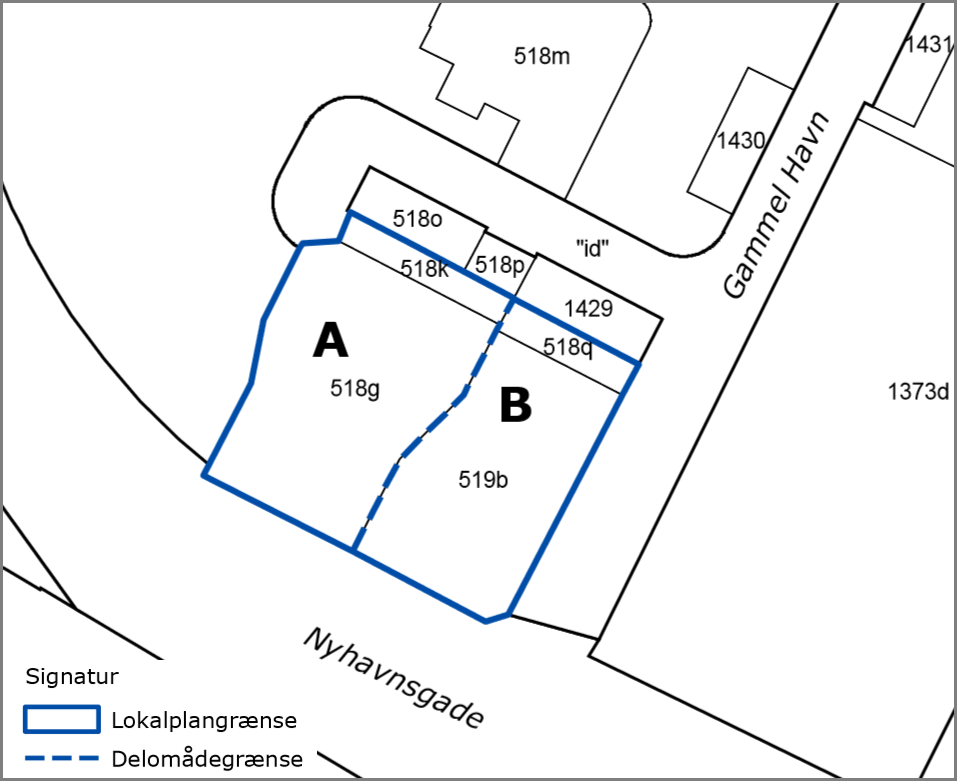
\includegraphics[width=0.7\textwidth]{billeder/tilbygning.png}
	\caption{Lokalplan 1-1-107, delområde A og B \citep[ bilag 1, s. 33]{lokalplan}}
	\label{fig:aogb}
\end{figure}

Da lokalplanområdet ligger meget kystnært skal der i større grad dimensioneres efter klimatiske faktorer og ændringer. Her er hovedpunktet vandstandsstigning. Her tages der udgangspunkt i Aalborg Kommunes klimastrategi. Den forudsiger, at den generelle indre vandstand i nordjyske farvande vil kunne stige med op til 1 m. Derfor er der fastsat en minimum sokkelkote for stueplan på nye bygninger på 2,36 m DVR 90 grundet risikoen for vandstandsstigning \citep[ s. 9]{lokalplan}.
\newline \indent{     }  Bygningen ligger placeret tæt op ad detailhandel og erhverv. Området benyttes af kollektiv trafik. Da bygningen ligger placeret ved Nyhavnsgade, kan dette give støjgener fra trafikken. Derfor skal der tages højde for dette, når der bygges. Det indendørs støjniveau må ikke overstige $L_{den}$ 33 dB, og ved udendørs opholdsarealer må den ikke overstige $L_{den}$ 58 dB. Støjisolering skal primært ske indvendigt, så bygningen ikke ændrer udseende. Overholdelse af de forskellige grænseværdier for støj skal kunne dokumenteres, før bygningen må tages i brug \citep[ s. 8]{lokalplan}. Området er kortlagt på vidensniveau 1 og 2 efter jordforureningsloven. Et areal bliver kortlagt på vidensniveau 1, hvis der er kendskab til aktiviteter, der kan forårsage forurening på arealet. Det vil blive kortlagt på vidensniveau 2, hvis der er dokumentation for forurening i jord og grundvand på arealet \citep{vidensniveau}. Hvis der i forbindelse med bygge- og anlægsarbejde konstateres tegn på jordforurening, skal arbejdet standses og kommunens Teknik- og Miljøforvaltning skal underrettes. Herefter vurderes det, om der skal fastsættes vilkår, inden arbejdet kan genoptages \citep[ s. 10]{lokalplan}.
\newline
\newline
Lokalplanen skal udarbejdes i samspil med den nuværende kommuneplan og anden fysisk planlægning i området omkring. Planen er, at der i lokalplanens område kan indrettes et mindre antal boliger. Det forventes at Aalborg Midtby får etableret 2.116 nye boliger i perioden 2008-2019. I bygningen kan desuden etableres butikker på maksimalt 250 $m^2$  og 500 $m^2$ pr. etage jf. kommuneplanen \citep[ s. 8]{lokalplan}.

\subsection{Fra gammel til ny lokalplan}
I kraft med vedtagelsen af lokalplan 1-1-107 ophæves lokalplanen 10-082 for det område, som lokalplan 1-1-107 omfatter. På trods af, at de to lokalplaner omfatter to forskellige områdestørrelser, så er lokalplanerne fortsat ens på flere punkter, heriblandt miljøforholdene for området. Der er dog nogle små forskelle, og disse forskelle vil blive analyseret i det følgende afsnit. Nedenfor på Figur \ref{fig:10-082} ses lokalplanområdet for lokalplan 10-082.

\begin{figure}[htbp]
	\centering
	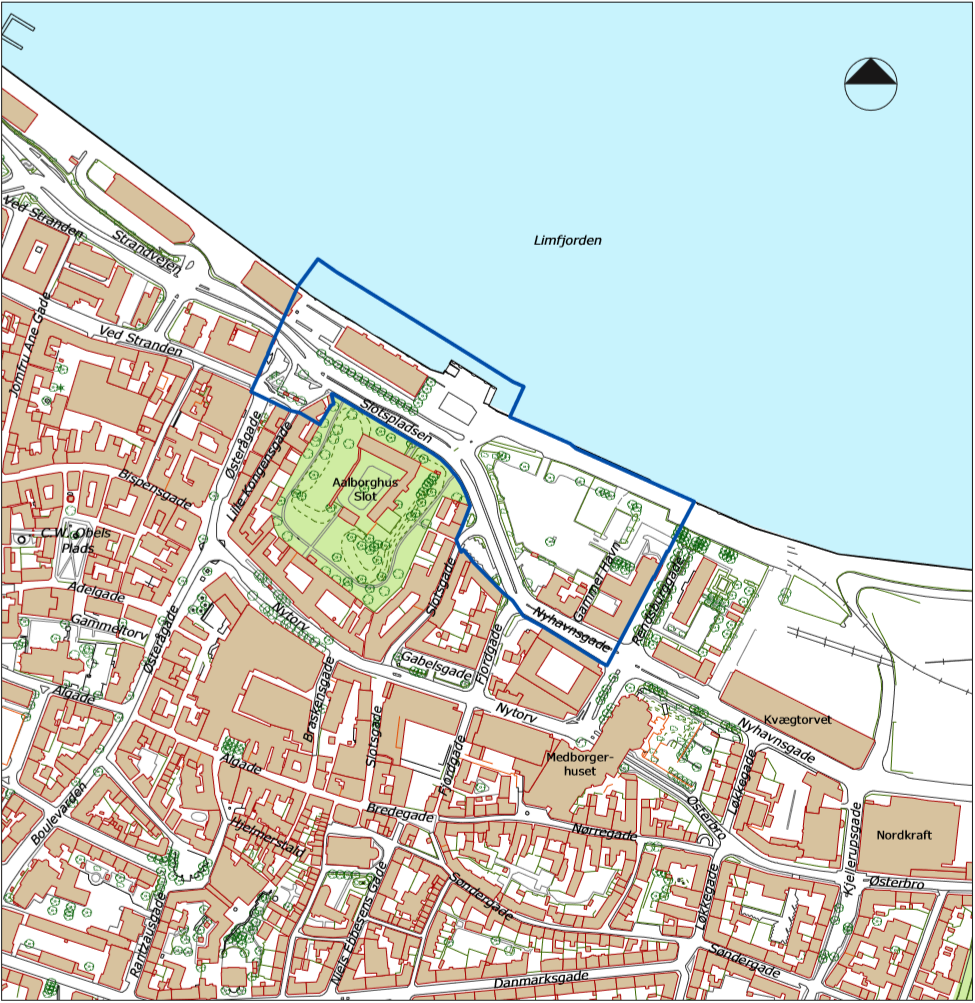
\includegraphics[width=0.5\textwidth]{billeder/lokalplanoversigt.png}
	\caption{Tidligere gældende lokalplan, 10-082, for området \citep[ s. 17]{gammellokalplan}}
	\label{fig:10-082}
\end{figure}

I lokalplan 10-082 kan ny bebyggelse for området Strøybergs Palæ bygges i 4 etager samt tagetage med en maksimal højde på 22 m \citep[ s. 19]{gammellokalplan}, hvor der i lokalplan 1-1-107 kan bygges i op til 3 etager samt tagetage for ny bebyggelse med en maksimal højde på 19 m. Denne ændring i højden kan skyldes, at der har været indsigelser imod de 22 m, da dette muligvis ville fjerne en udsigt eller sollys for de berørte personer. 
\newline \indent{     }  Der er i lokalplan 1-1-107 ligeledes taget højde for vandstandsstigning i Limfjorden, hvilket ikke er gjort i lokalplan 10-082. Grunden til dette kan skyldes, at der ikke tages højde for detaljerne, da lokalplan 10-082 foruden Strøybergs Palæ indeholder tiltag til Utzon Centeret, Slotspladsen og First Slotshotel.
\newline \indent{     }  Ligeledes bliver der præciseret i lokalplan 1-1-107, at isolering for trafikstøj ikke må ændre på facadens udseende, hvor der i lokalplan 10-082 blot står, at enhver ændring på bygningens facade kræver en tilladelse \citep[ s. 19]{gammellokalplan}. En grund til at der først i lokalplan 1-1-107 står beskrevet, hvordan isoleringen skal foretages samt at facadeændringer kræver en tilladelse, kan være, at lokalplan 10-082 dækker over et større område end 1-1-107, og at detaljerne på tilbygningen dermed først er relevant for lokalplan 1-1-107. 
\newline \indent{     }  For ny bebyggelse og nye tilbygninger, som er omfattet af lokalplan 1-1-107, gælder det, at nye bygninger skal opføres i overensstemmelse med den eksisterende bebyggelse, dog gerne med nutidig arkitektonisk formsprog. Tilbygninger skal opføres i tilknytning til den eksisterende bevaringsværdige bygning, og skal derfor have det samme arkitektoniske udtryk, som bygningen i forvejen har \citep[ s. 7]{lokalplan}. 
\newline \indent{     }  Dette punkt i lokalplanen forklarer de overordnede rammer for ny bebyggelse og tilbygning, men udover dette, er det mere frit for det pågældende rådgivningsfirma, at designe og konstruere de pågældende bygninger. De skal blot overholde lokalplanens givne rammer, hvorefter det kan diskuteres og fortolkes, hvor og hvornår grænsen for det arkitektoniske udtryk overskrides. Denne balance er derfor mest op til det rådgivende ingeniørselskab at fortolke.

\section{Delkonklusion}
Der er i de foregående afsnit redegjort for Aalborgs historie og baggrunden for byens udvikling. Ligeledes er der beskrevet, hvad en kommuneplan og lokalplan er, og der er lavet en dybdegående analyse af Aalborgs kommuneplan, med særligt fokus på Vækstaksen. Inden for vækstaksen ligger Strøybergs Palæ, som hører under den nuværende lokalplan 1-1-107, hvilken også er behandlet, analyseret og sammenlignet med den tidligere lokalplan for området, 10-0-82. Endelig er der foretaget en diskussion, hvor spørgsmålet stilles, hvorfor det er godt at udvikle i netop dette område, og derunder hvilken sammenhæng der er mellem Strøybergs Palæ og Vækstaksen.
\newline
\newline
Kommuneplanen er den overordnede ramme for byens udvikling, mens lokalplanen beskriver et mindre område inden for kommunen, og har til formål at styre udviklingen af dette. Aalborg Kommune er vokset som by gennem tiden, og gennem den nuværende kommuneplan
har kommunen en målsætning om, at blive Nordjyllands Vækstdynamo og blive en
by med fokus på udvikling af studerende, erhverv, kultur med mere. 
\newline \indent{     }  Blandt Aalborg Kommunes fem fokuspunkter er det fokuspunktet “Aalborg - den attraktive storby”, omhandlende Vækstaksen, der er blevet behandlet. Vækstaksen beskriver et område i Aalborg, hvor der er planer om fremtidig udvikling. Disse områder består i dag af virksomheder, uddannelsesinstitutioner, kulturattraktioner og andre interessepunkter for Aalborg Kommune. Det er netop disse område, der skal skabe grobund for den fremtidige vækst i Aalborg, og derfor er det fordelagtigt at udvikle yderligere i netop disse områder.
\newline \indent{     }  Et af hovedpunkterne i Vækstaksen er, at udvikle Aalborg gennem en byfortætning, hvor målet er at få flere virksomheder og indbyggere til byen. En tilbygning af Strøybergs Palæ vil give ekstra erhvervslokaler og lejligheder, hvilket passer godt sammen med kommunens ønske om byfortætning. 
\newline
\newline
Med en beliggenhed inden for Vækstaksen i et af de områder, hvor der er størst mulighed for udvikling, er der grundlag for en udvidelse af Strøybergs Palæ. Derudover har de seneste 10 års udvikling af havnefronten, givet øget fokus på udviklingen i dette område, hvilket  gør området mere attraktivt. Dette er et godt grundlag for at lave en tilbygning, som vil give ekstra plads og bedre forudsætninger for udviklingen. Tilbygningen kan blandt andet bruges til erhvervslokaler, som kan tiltrække nye virksomheder til områder, og dermed være med til at udvikle byen.  Dog vil en mindre udvidelse af Strøybergs Palæ ikke have en stor betydning for Aalborg og dens udvikling, da bygningen kun er en lille del af Vækstaksen.

%% Kontekst %%



%% Teknisk %%

\chapter{Dimensionering}

Figur \ref{fig:hej} viser de nye byggefelter inden for henholdsvis delområde A og delområde B til Strøybergs Palæ (\citep{lokalplan}, s. 16). Denne rapport fokuserer på byggefeltet inden for delområde B, hvor ny bebyggelse, ifølge lokalplan 1-1-107, må opføres i 3 etager samt en tagetage og med en kælder maksimalt 2 m over terræn. Ved opførsel af ny bebyggelse i delområde B, skal to nuværende mindre bygninger fjernes. 

\begin{figure}[htbp]
	\centering
	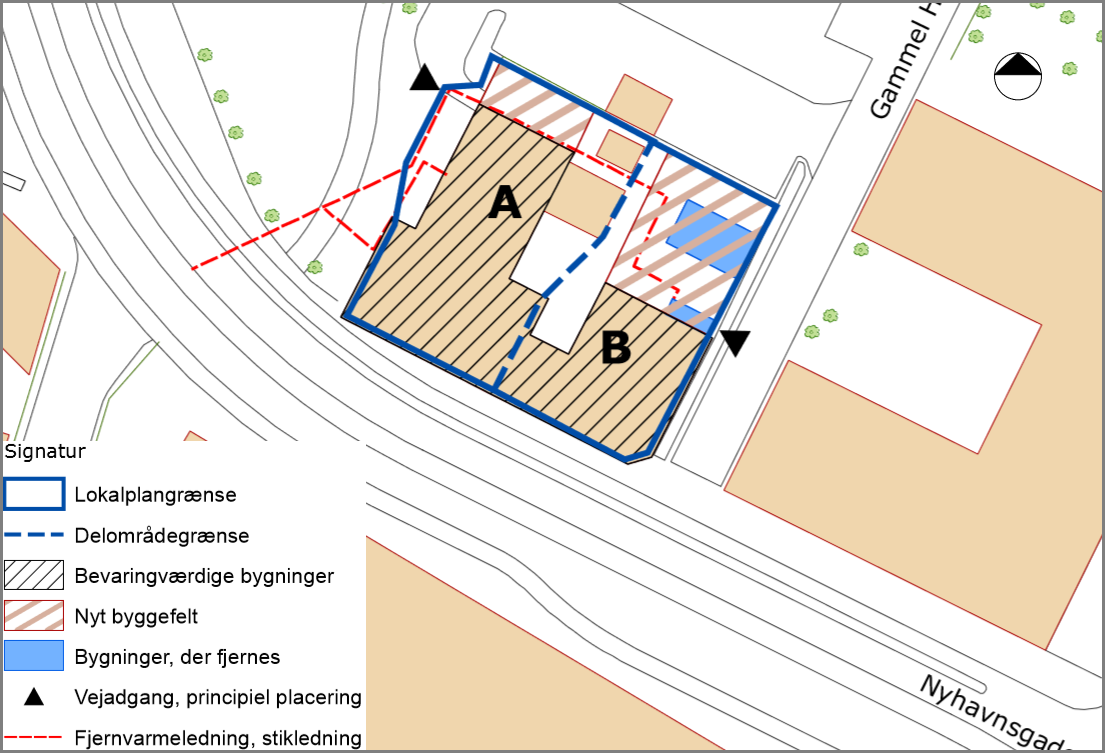
\includegraphics[width=0.7\textwidth]{billeder/signatur.png}
	\caption{Lokalplan 1-1-107, delområde A og B}
	\label{fig:hej}
\end{figure}

Med udgangspunkt i lokalplan 1-1-107 har bygningen fået de størrelser og dimensioner, som ses på Figur \ref{fig:farvel}.
\newline \indent{     }  Tilbygningen bliver 12,5 meter lang og 12 meter bred i henhold til den eksisterende bygningsbredde. Kælderen har en højde på i alt 3,25 m, hvor 1,25 m ligger over terræn. Stueetagen, 1. sal og 2. sal har hver især en højde på 4,9 m og tagetagen har en højde på 3 meter med en hældning på 26,6 grader. I alt er tilbygningen 19 m høj over terræn.

\begin{figure}[htbp]
	\centering
	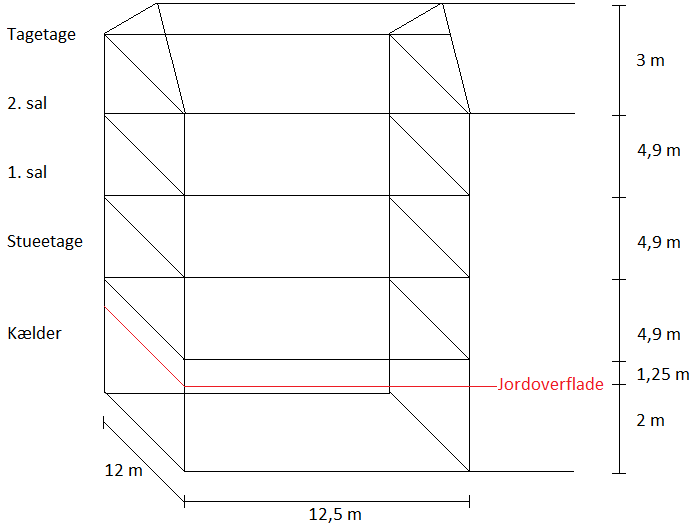
\includegraphics[width=0.7\textwidth]{billeder/tilbygning2.png}
	\caption{Tilbygningens dimensioner}
	\label{fig:farvel}
\end{figure}

For at kunne beregne de laster som påvirker tilbygningen, er der opstillet nedenstående statisk system for bygningen. Systemet er opstillet som en bjælkekonstruktion.
\newline
\newline
FIGURE HER!

\section{Laster}
Lidt tekst her.

\subsection{Permanent last}
Indsætte her.

\subsection{Variable laster}
Af variable laster optræder der både snelast og vindlast på bygningen, og disse udregnes efter Dansk Standard Eurocode 1991.

\subsubsection{Snelast}
Til at beregne hvordan snelasten påvirker tilbygningen anvendes den karaktiske snelast og formlen:
\begin{center}
$s=\mu_i\cdot C_e\cdot C_t \cdot s_k$
\end{center}
\begin{itemize}
	\item[-] $s$: karakteristisk snelast
	\item[-] $\mu_i$: formfaktoren for snelasten, som sættes til 0.8 (\citep{EU91}, tabel 5.2 s. 53)
	\item[-] $C_e$: eksponeringsfaktoren
	\item[-] $C_t$: termisk faktor, som sættes til 1.0 (\citep{EU91}, s. 52)
	\item[-] $s_k$: karakteristisk terrænværdi, som sættes til $1 \frac{kN}{m^2}$ (\citep{EU91}, s. 49)
\end{itemize}
Til at bestemme den karakteristiske snelast, beregnes eksponeringsfaktoren $C_e$.
\newline
\newline
Eksponeringsfaktoren, $C_e$, bestemmes ved:
\begin{center}
$C_e=C_{top}\cdot C_s$
\end{center}
\begin{itemize}
	\item[-] $C_{top}$: topografi faktor, som sættes til 1.0 (\citep{EU91}, tabel 5.1 s. 51)
	\item[-] $C_s$: størrelse faktor, som sættes til 1.0 (\citep{EU91}, s. 51-52)
\end{itemize}
Eksponeringsfaktoren kan nu bestemmes til:
\begin{center}
$C_e=1.0\cdot 1.0=1.0$
\end{center}
Strøybergs Palæ har et saddeltag, og dermed skal der tages højde for tre lasttilfælde, som ses på Figur INDSÆTTE FIGUR!
\newline
\newline
\underline{Lasttilfælde 1}
\begin{center}
$s_1=0.8\cdot 1.0\cdot 1.0\cdot 1 \frac{kN}{m^2}=0.8 \frac{kN}{m^2}$
\end{center}
\underline{Lasttilfælde 2 og 3}
\begin{center}
$s_2=\frac{1}{2}\cdot 0.8\cdot 1.0\cdot 1.0\cdot 1 \frac{kN}{m^2}=0.4 \frac{kN}{m^2}$
\end{center}
\underline{Lasttilfælde 4}
\begin{center}
	$s_4=\mu_w\cdot C_e\cdot C_t\cdot s_k \frac{kN}{m^2}$
\end{center}
\begin{itemize}
	\item[-] $\mu_w$: formfaktoren, som sættes til 1.2 eftersom $\alpha$ er $26.565^{\circ}$ (\citep{EU91}, s. 55)
\end{itemize}
Den karakteristiske snelast for lasttilfælde 4 kan nu bestemmes til:
\begin{center}
	$s_4=1.2\cdot 1.0\cdot 1.0\cdot 1 \frac{kN}{m^2}=1.2 \frac{kN}{m^2}$
\end{center}
I og med at lasttilfælde 4 giver den største last, anvendes denne til videre beregning.

\subsubsection{Vindlast}
Vindlasten beregnes for det højeste punkt på konstruktionen, hvilket er på tagspidsen for tilbygningen, da det er det punkt, hvor vinden er kraftigst.
\newline
\newline
FIGUR! - henvis til den med taget, som skal være i egenlasten
\newline
\newline
Til at bestemme vindlasten på tilbygningen bruges følgende formel:	
\begin{center} $w_e=q_p(z_e)$$\cdot$$c_{pe}$
\end{center}
\begin{itemize}
	\item[-] $q_p$: peakhastighedstrykket
	\item[-] $z_e$: referencehøjden for det udvendige vindtryk
	\item[-] $c_{pe}$: formfaktoren for det udvendige vindtryk
\end{itemize}
Den maksimale belastning fra vinden, peakhastighedstrykket $q_p$, bestemmes ved:
\begin{center}
$q_p(z_e)=[1+7I_v(z_e)]$$\cdot$$\frac{1}{2}$$\cdot$p$\cdot$$v_m^2(z_e)$
\end{center}
\begin{itemize}
	\item[-] $I_v$: vindturbulens
	\item[-] $\rho$: densiteten for luft $1.25 \frac{kg}{m^3}$
	\item[-] $v_m$: middelvindhastigheden
\end{itemize}
For at bestemme peakhastigheden, beregnes først vindturbulens $I_v(z)$ samt middelvindhastigheden $v_m$.
\newline
\newline
Vindturbulens, $I_v(z)$, bestemmes ved:
\begin{center}
$I_v(z)=\frac{\sigma_v}{V_m(z)}=\frac{k_1}{c_0(z)\cdot ln(\frac{z}{z_0})}$
\end{center}
\begin{itemize}
	\item[-] $k_1$: turbulensfaktor, sættes til 1.0 (\citep{EU91}, s. 82)
	\item[-] $c_0(z)$: orografifaktoren, som sættes til 1.0 (\citep{EU91}, s. 78)
	\item[-] $z$: højde, som er 19 m
	\item[-] $z_0$: ruhedslængde, som sættes til 1.0 for terrænkategori IV (\citep{EU91}, s. 79)
\end{itemize}
Vindturbulensen kan nu bestemmes til:
\begin{center}
$I_v(z)=\frac{1.0}{1.0\cdot ln(\frac{19}{1.0})}=0.340$
\end{center}
Middelvindhastigheden, $v_m$, bestemmes ved:
\begin{center}
$v_m(z)=c_r(z)\cdot c_0(z)\cdot v_b$
\end{center}
\begin{itemize}
	\item[-] $c_r(z)$: ruhedsfaktor
	\item[-] $v_b$: basisvindhastigheden
\end{itemize}
Til at bestemme middelvindhastigheden, beregnes basisvindhastigheden samt ruhedsfaktor.
\newline
\newline
Basisvindhastigheden, $v_b$, bestemmes ved:
\begin{center}
$v_b=c_{dir}\cdot c_{season}\cdot v_{b,0}$
\end{center}
\begin{itemize}
	\item[-] $c_{dir}$: retningsfaktor, som sættes til 1.0 (\citep{EU91}, tabel 1a s. 77)
	\item[-] $c_{season}$: årstidsfaktor, som sættes til 1.0 (\citep{EU91}, tabel 1b s. 77)
	\item[-] $v_{b,0}$: grundværdi for basisvindhastigheden, som sættes til 24 $\frac{m}{s}$, da dette er gældende for størstedelen af Danmark (\citep{EU91}, s. 77)
\end{itemize}
Basisvindhastigheden kan nu bestemmes til:
\begin{center}
$v_b=1.0\cdot 1.0\cdot 24 \frac{m}{s}=24 \frac{m}{s}$
\end{center}
Ruhedsfaktor, $c_r(z)$, bestemmes ved:
\begin{center}
$c_r(z)=k_r\cdot ln(\frac{z}{z_0})$
\end{center}
\begin{itemize}
	\item[-] $k_r$: terrænfaktor
\end{itemize}
Terrænfaktoren, $k_r$, bestemmes ved:
\begin{center}
$k_r=0.19\cdot (\frac{z_0}{z_{0,II}})^{0.07}$
\end{center}
\begin{itemize}
	\item[-] $z_{0,II}$: værdi for ruhedslængde for terrænkategori II, som sættes til 0.05 (\citep{EU91}, s. 78-79)
\end{itemize}
\begin{center}
$k_r=0.19\cdot (\frac{1.0}{z_{0.05}})^{0.07}=0.234$
\end{center}
Ruhedsfaktor kan nu bestemmes til:
\begin{center}
$c_r(z)=0.234\cdot ln(\frac{19}{1.0})=0.690$
\end{center}
Middelvindhastigheden kan nu bestemmes til:
\begin{center}
$v_m(z)=0.690\cdot 1.0\cdot 24 \frac{m}{s}=16.569 \frac{m}{s}$
\end{center}
Peakhastighedstrykket $q_p$ i højden z, kan nu bestemmes til:
\begin{center}
$q_p(z_e)=[1+7\cdot 0.340]\cdot \frac{1}{2}\cdot 1.25 \frac{kg}{m^3}\cdot (16.569 \frac{m}{s})^2=0.579 \frac{kN}{m^2}$
\end{center}

HVAD GØR VI NU??

\begin{figure}[htbp]
	\centering
	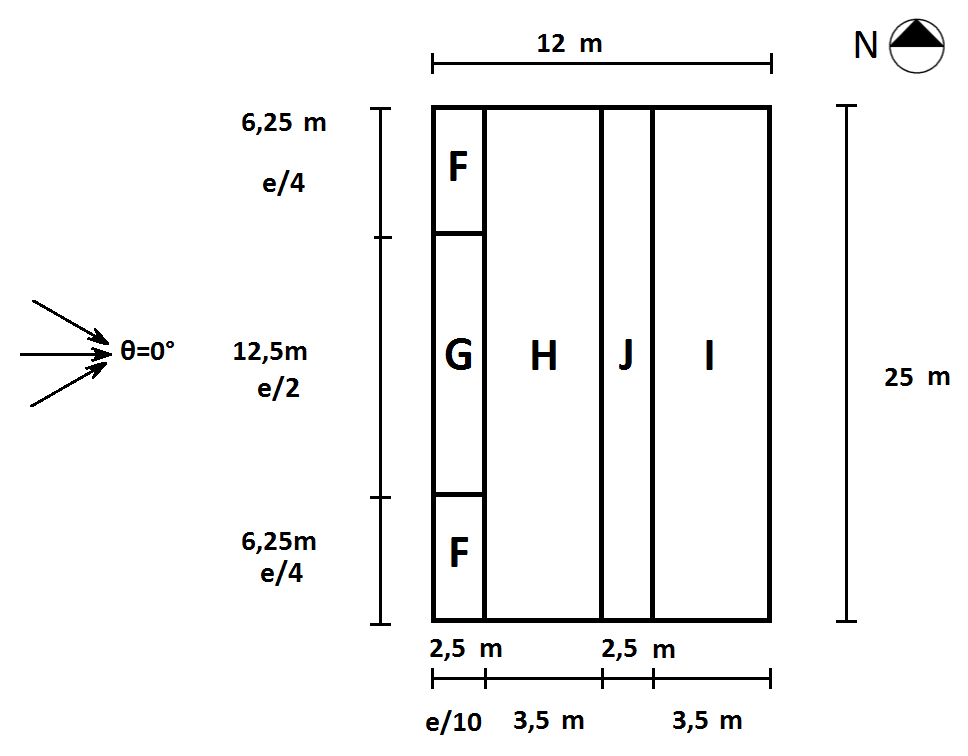
\includegraphics[width=0.5\textwidth]{billeder/opdeling.png}
	\caption{Zoneinddeling af taget}
	\label{fig:tag}
\end{figure}

For alle zoner bestemmes $c_{pe,10}$. Der opstilles en lineær ligning med sammenhæng mellem $c_{pe,10}$ værdierne og graderne 15 og 30. Herefter indsættes taghældningen, $26.565^{\circ}$ i ligningen og værdien for $c_{pe,10}$ i den pågældende zone fås.
\newline
\newline
\underline{Zone F}
\newline
Ud fra tabel 7.4a (\citep{EU91}, s. 112) er de negative værdier for zone F -0.9 og -0.5. Her ud fra fås ligningen, og $c_{pe,10,neg}$ bestemmes:
\begin{center}
	$f(\alpha)=0.0267\cdot \alpha - 1.3 \to c_{pe,10,neg}=-0.592$
\end{center}
De positive værdier for zone F er: 0.2 og 0.7. Her ud fra fås ligningen, og $c_{pe,10,pos}$ bestemmes:
\begin{center}
	$f(\alpha)=0.0333\cdot \alpha - 0.3 \to c_{pe,10,pos}=0.585$
\end{center}

\underline{Zone G}
\newline
De negative værdier for zone G er: -0.8 og -0.5. Her ud fra fås ligningen, og $c_{pe,10,neg}$ bestemmes:
\begin{center}
	$f(\alpha)=0.02\cdot \alpha - 1.1 \to c_{pe,10,neg}=-0.569$
\end{center}
De positive værdier for zone G er: 0.2 og 0.7. Her ud fra fås ligningen, og $c_{pe,10,pos}$ bestemmes:
\begin{center}
	$f(\alpha)=0.0333\cdot \alpha - 0.3 \to c_{pe,10,pos}=0.585$
\end{center}

\underline{Zone H}
\newline
De negative værdier for zone H er: -0.3 og -0.2. Her ud fra fås ligningen, og $c_{pe,10,neg}$ bestemmes:
\begin{center}
	$f(\alpha)=0.00667\cdot \alpha - 0.4 \to c_{pe,10,neg}=-0.223$
\end{center}
De positive værdier for zone H er: 0.2 og 0.4. Her ud fra fås ligningen, og $c_{pe,10,pos}$ bestemmes:
\begin{center}
	$f(\alpha)=0.0133\cdot \alpha - 1.178\cdot 10^{-16} \to c_{pe,10,pos}=0.354$
\end{center}

\underline{Zone I}
\newline
Den negative værdi for zone I er: -0.4. Her ud fra fås ligningen, og $c_{pe,10,neg}$ bestemmes:
\begin{center}
	$f(\alpha)=-5.234\cdot 10^{-18}\cdot \alpha - 0.4 \to c_{pe,10,neg}=-0.4$
\end{center}
Den positive værdi for zone I er: 0.0. Her ud fra fås ligningen, og $c_{pe,10,pos}$ bestemmes:
\begin{center}
	$f(\alpha)=0.0 \to c_{pe,10,pos}=0.0$
\end{center}

\underline{Zone J}
\newline
De negative værdier for zone J er: -1.0 og -0.5. Her ud fra fås ligningen, og $c_{pe,10,neg}$ bestemmes:
\begin{center}
	$f(\alpha)=0.0333\cdot \alpha - 1.5 \to c_{pe,10,neg}=-0.615$
\end{center}
Den positive værdi for zone J er: 0.0. Her ud fra fås ligningen, og $c_{pe,10,pos}$ bestemmes:
\begin{center}
	$f(\alpha)=0.0 \to c_{pe,10,pos}=0.0$
\end{center}
INDSÆTTE DET SIDSTE!

\section{Lastkombinationer}
INTROTEKST
\newline
\newline
\underline{Egenlast}
\newline
Egenlasten bestemmes ud fra følgende formel:
\begin{center}
	$E_{d,1}=\gamma_{G1}\cdot K_{FI}\cdot G_{K1}$
\end{center}
\begin{itemize}
	\item[-] $E_{d,1}$: regningsmæssige egenlast
	\item[-] $\gamma_{G1}$: partialkoefficienten for den permanente last, som sættes til 1.0 (\citep{EU90}, tabel A 1.2 s. 44)
	\item[-] $K_{FI}$: konsekvensklasse CC3, som sættes til 1.1 (\citep{EU90}, s. 43)
	\item[-] $G_{K1}$: karakteristisk egenlast for den permanente last [kN], som sættes til 3437.84 kN
\end{itemize}
Egenlasten kan nu bestemmes til:
\begin{center}
	$E_{d,1}=1.0\cdot 1.1\cdot 3437.84 kN=4.538\cdot 10^3 kN$
\end{center}
\underline{Vindlast dominerende}
\newline
Nyttelasten for vindlast dominerende kan bestemmes ud fra følgende formel:
\begin{center}
	$E_{d,2}=\gamma_{G1}\cdot K_{FI}\cdot G_{K1}+\gamma_{Q1}\cdot K_{FI}\cdot Q_{k,1}+\gamma_{Q2}\cdot \Psi_{0,2}\cdot K_{FI}\cdot Q_{k,2}$
\end{center}
\begin{itemize}
	\item[-] $E_{d,2}$: regningsmæssige last
	\item[-] $\gamma_{Q1}$: partialkoefficienten for den dominerende last(vindlast), som sættes til 1.5 (\citep{EU90}, tabel A 1.2 s. 44)
	\item[-] $Q_{k,1}$: karakteristisk nyttelast for vind, som sættes til TAL!!
	\item[-] $\gamma_{Q2}$: partialkoefficenten for den variable last(snelast), som sættes til 1.5 (\citep{EU90}, tabel A 1.2 s. 44)
	\item[-] $\Psi_{0,2}$: $\Psi$-faktor, som sættes til 0 (\citep{EU90}, tabel A 1.1 s. 41)
	\item[-] $Q_{k,2}$: karakteristisk nyttelast for sne, som sættes til TAL!!
\end{itemize}
Nyttelasten for vindlast dominerende kan nu bestemmes til:
\newline
\newline
INDSÆTTE!
\newline
\newline
\underline{Snelast dominerende}
Nyttelasten for snelast dominerende kan bestemmes ud fra følgende formel: 

\chapter{Brudgrænsetilstand}

I dette afsnit undersøges tilbygningens brudgrænsetilstand. Først beregnes reaktionerne ud fra Figur \ref{fig:alle} og dernæst laves snitkræfter. Slutteligt undersøges spændingstilstanden, og udfra ståltypens flydespændingen kan det vurderes, om konstruktionen kan holde eller vil bryde sammen.   

\section{Reaktioner}
Reaktionerne i de tre understøtninger beregnes ved at opdele konstruktionen. Systemet opdeles i det midterste charnierled i henholdvis en venstre- og højre del, som ses på Figur \ref{fig:opdelingv} og \ref{fig:opdelingh}. I skæringen mellem de to dele, vil der være snitkræfter, men ikke momentkræfter, da momentet i charnierledet er nul. Dermed optræder der kun normalkraften, N, og forskydningskraften, V. Det er derfor muligt, at betragte højre del som et isoleret del af konstruktionen med fast, simpel understøtning i punkt E.

\begin{figure}[H]
	\centering
	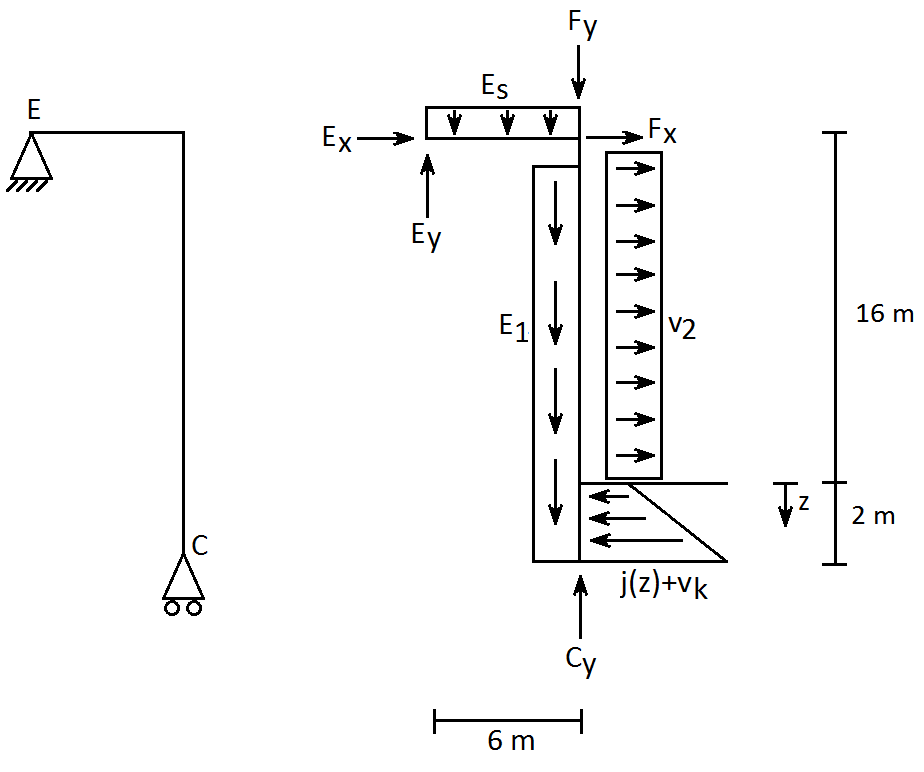
\includegraphics[width=0.7\textwidth]{billeder/hojre.png}
	\caption{Højre side af systemet, samt fritlegemediagram}
	\label{fig:opdelingh}
\end{figure}

\begin{figure}[H]
	\centering
	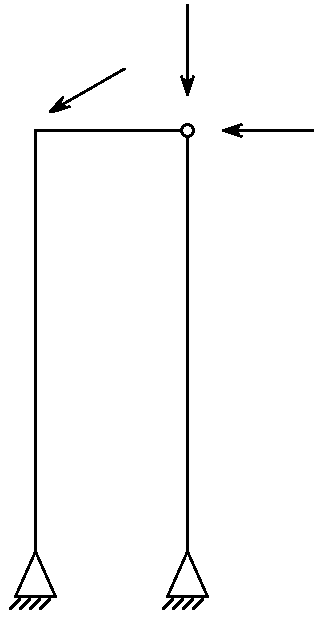
\includegraphics[width=0.7\textwidth]{billeder/venstre.png}
	\caption{Venstre side af systemet, samt fritlegemediagram}
	\label{fig:opdelingv}
\end{figure}

Reaktionerne i punkt E kan sættes som punktlaster på den venstre side af systemet, som ses på Figur \ref{fig:opdelingv}. Reaktionerne på højre del af systemet beregnes først.
\newline
\newline
Først bestemmes den vandrette reaktion i charnier ledet, $E_x$ gennem vandret ligevægt: 
\begin{center}
	$\rightarrow+:0 = F_x + E_x - J(2m) - V_k \cdot 2m - V_2 \cdot 16m$
	\newline
	$E_x = -1,\!45 kN$
\end{center}

$C_y$ bestemmes gennem moment ligevægt om punkt E: 
\begin{center}
	$\AR{}:0 = -F_y \cdot 6m - E_1 \cdot 18m \cdot 6m + C_y \cdot 6m - J(2m) \cdot 17,\!33m - V_k \cdot 2m \cdot 17m - E_s \cdot 6m \cdot 3m - V_2 \cdot 16m \cdot 8m$
	\newline
	$C_y = 779,\!83 kN$
\end{center}

Til sidst bestemmes den lodrette reaktion i charnier ledet, $E_y$ gennem lodret ligevægt: 
\begin{center}
	$\uparrow+: 0 = F_y - E_1 \cdot 18m - E_s \cdot 6m + C_y + E_y$
	\newline	
	$E_y = -164,\!89 kN$
\end{center}

Reaktionerne $E_y$ og $E_x$ påsættes som belastninger i punkt E på det venstre system, så de virker som vist på Figur \ref{fig:opdelingv}. Reaktionerne i det venstre system kan hermed bestemmes.
\newline
\newline
Først tages der moment om A, for at beregne $B_y$:
\begin{center}
	$A\hookrightarrow+: 0 = B_y \cdot 6m + E_y \cdot 6m + E_x \cdot 18m - E_2 \cdot 18m \cdot 6m - E_s \cdot 6m \cdot 3m + D_x \cdot 18m - V_1 \cdot 16m \cdot (8m + 2m) - J(2m) \cdot (2m \cdot \frac{1}{3}) - V_k \cdot 2m \cdot 1m$
	\newline 
	$B_y = 127,\!92 kN$
\end{center}

Nu laves lodret ligevægt for at bestemme $A_y$:
\begin{center}
	$\uparrow+: 0 = A_y + B_y - E_y - E_2 \cdot 18m - E_1 \cdot 18m - F_y - E_s \cdot 6 m$
	\newline
	$A_y = 547,\!96 kN$
\end{center}

For at gøre det muligt at isolere en af de vandrette reaktioner laves der et snit i charnieret. Derefter betragtes den nedre del, og der tages moment omkring charnieret i punkt E, for at bestemme $B_x$:
\begin{center}
	$\hookrightarrow+: 0 = B_x \cdot 18m$
	\newline
	$B_x = 0 kN$
\end{center}

Slutteligt laves vandret ligevægt for at bestemme $A_x$:
\begin{center}
	$\rightarrow+: 0 = A_x - E_x + B_x + J(2m) + V_k \cdot 2m + V_1 \cdot 16 m - D_x$
	\newline
	$A_x = -133,\!31 kN$
\end{center} 

\section{Snitkræfter}
Snitkræfterne for stålrammen til tilbygningen til Strøybergs Palæs kan nu beregnes. Her laves der syv snit, som er illustreret på Figur \ref{fig:snitbrud}. Disse resultater vil bruges til at undersøge, om konstruktionen har en tilstrækkelig bæreevne, eller om den vil bryde sammen. 

\begin{figure}[H]
	\centering
	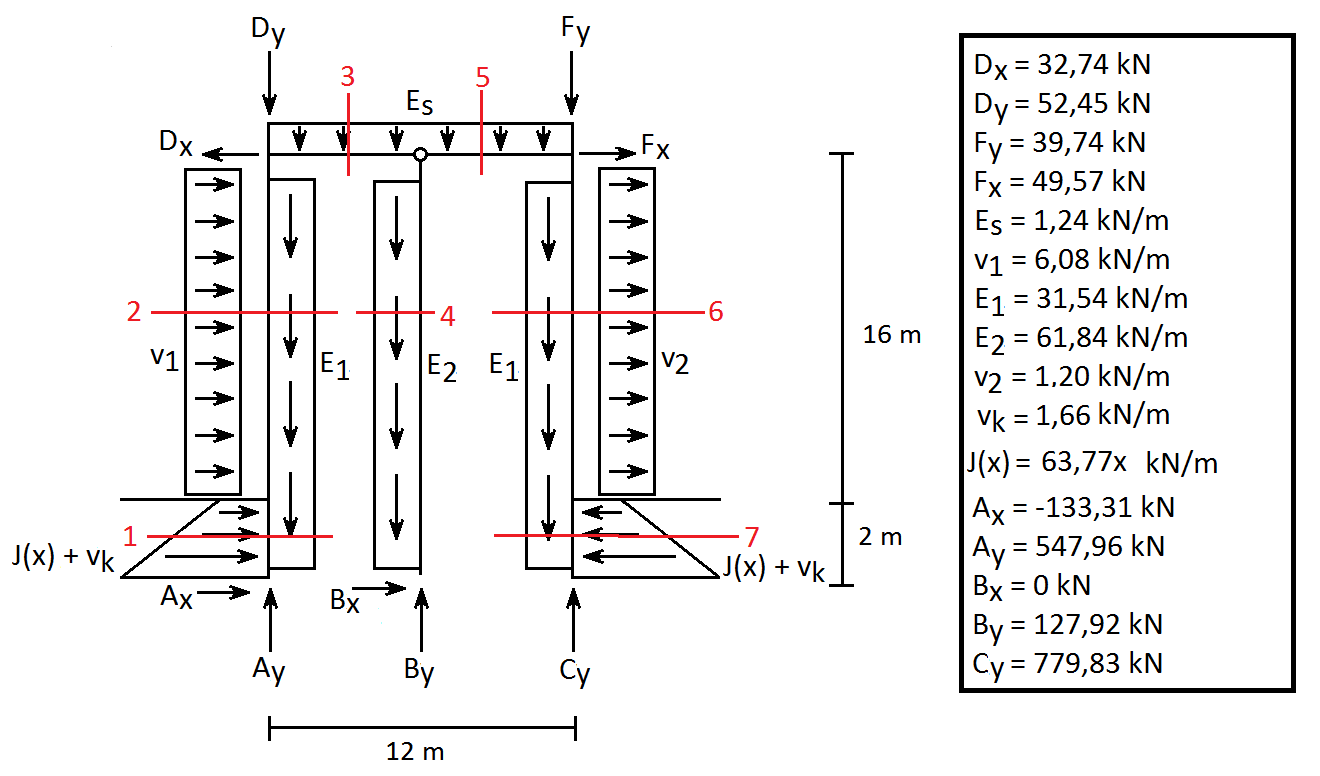
\includegraphics[width=0.8\textwidth]{billeder/snitbrud.png}
	\caption{Snit}
	\label{fig:snitbrud}
\end{figure}

Nedenfor vises beregningseksempel for snit 1 og snit 5. Beregningerne for de resterende snit kan ses i Bilag ???. 
\newline
\newline
\textbf{Snit 1: 0 m < x < 2 m}
\newline
Fritlegemediagrammet for snit 1 ses på Figur \ref{fig:snitet}.
\newline
\newline
Først bestemmes normalkraften:
\begin{center}
	$0 = N_1 + A_y - E_1 \cdot x \leftrightarrow N_1(x) = 31,\!54 \frac{kN}{m} x - 547,\!95 kN $
\end{center}

Normalkraften bestemmes ved 0 m og 2 m:
\begin{center}
	$N_1(0m) = -547,\!95 kN$ og	$N_1(2m) = -484,\!87 kN$
\end{center}

Nu bestemmes forskydningskraften:
\begin{center}
	$0 = V_1 + J(x) + v_k \cdot x + A_x \leftrightarrow V_1(x) = -33,\!64\frac{kN}{m} x + 133,\!31 kN$
\end{center}

Forskydningskraften bestemmes ved 0 m og 2 m:
\begin{center}
	$V_1(0m) = 133,\!31 kN$ og $V_1(2m) = 66,\!02 kN$
\end{center}

Til sidst bestemmes momentkraften:
\begin{center}
	$0 = M_1 + J(x) \cdot \frac{2x}{3} + v_k \cdot x \cdot \frac{x}{2} + A_x \cdot x \leftrightarrow M_1(x) = -22,\!15\frac{kN}{m} x^2 + 133,\!30kN x$
\end{center}

Momentkraften i højden 0 m og 2 m bestemmes:
\begin{center}
	$M_1(0m) = 0 kNm$  og $M_1(2m) = 178,\!00 kNm$
\end{center}

\begin{figure}[H]\centering
	\begin{minipage}[b]{0.48\textwidth}\centering
		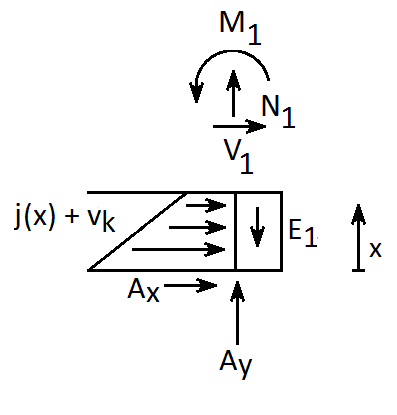
\includegraphics[width=0.80\textwidth]{billeder/snitet.png} %Venstre billede
	\end{minipage}\hfill
	\begin{minipage}[b]{0.48\textwidth}\centering
		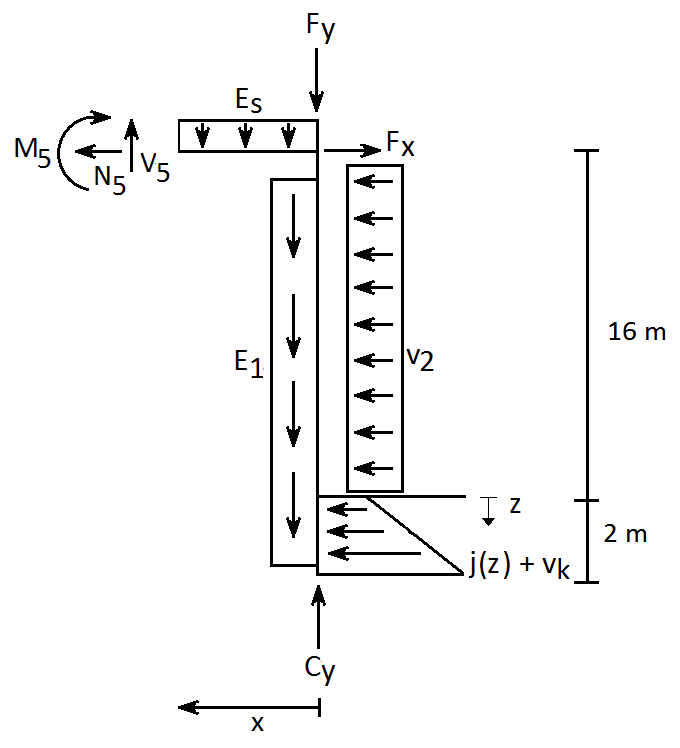
\includegraphics[width=1.0\textwidth]{billeder/snitfem.png} %Højre billede
	\end{minipage}\\ %Captions and labels
	\begin{minipage}[t]{0.48\textwidth}
		\caption{Fritlegemediagram for snit 1} %Venstre caption og label
		\label{fig:snitet}
	\end{minipage}\hfill
	\begin{minipage}[t]{0.48\textwidth}
		\caption{Fritlegemediagram for snit 5} %Højre caption og label
		\label{fig:snitfem}
	\end{minipage}
\end{figure}

\textbf{Snit 5: 0 m < x < 6 m}
\newline
Fritlegemediagrammet for snit 1 ses på Figur \ref{fig:snitfem}.
\newline
\newline
Normalkraften bestemmes først:
\begin{center}
	$0 = -N_5 + F_x - v_2 \cdot 16m - J(2m) - v_k \cdot 2m \leftrightarrow N_5 = 49,\!57 kN - 48,\!12 kN = 1,\!45 kN$
\end{center}

Hermed er normalkraften til 0 m og 6 m 1,45 kN. 
\newline
\newline
Forskydningskraften for snit 5 bestemmes ved:
\begin{center}
	$0 = V_5 - E_1 \cdot 18 m - F_y + C_y - E_s x \leftrightarrow V_5(x) = -172,\!35 kN + 1,\!24 \frac{kN}{m}x$
\end{center}

Forskydningskraften til 0 m og 6 m er hermed:
\begin{center}
	$V_5(0m) = -172,\!35 kN$ og $V_5(6m) = -164,\!89 kN$
\end{center}

Til sidst bestemmes momentkraften:
\begin{center}
	$0 = -M_5 - F_y \cdot x - E_1 \cdot 18 m \cdot x - E_s \cdot x \frac{x}{2} - v_2 \cdot 16 m \cdot 8 m - v_k \cdot 2 m \cdot 17 m - J(2m) \cdot 17,\!33 m + C_y \cdot x \leftrightarrow M_5(x) = 172,\!35 kN \cdot x - 0,\!62 \frac{kN}{m} \cdot x^2 -1011,\!72 kNm$
\end{center}

Momentkraften til 0 m og 6 m bestemmes:
\begin{center}
	$M_5(0m) = -1011,\!72 kNm$ og $M_5(6m) = 0 kN$
\end{center}

Tabel \ref{tab:resultaterbrud} viser resultaterne for alle snittene, som bruges til at beregne spændingstilstanden. 

\begin{table}
	\begin{center}
		\begin{tabular}{|c|c|c|c|c|c|c|}
			\hline
			Snit/Værdi & N($x_{min}$) & N($x_{max}$) & V($x_{min}$) & V($x_{max}$) & M($x_{min}$) & M($x_{max}$) 	\\ \hline
			1, 0<x<2  & -547,95       & -484,87    	&  133,31    	&  66,02 	&  0,00     &  178.00        		\\ \hline
			2, 2<x<18 &  -484,87        &  19,78       &  53,85      & -43,46   &  178,00  &  455,80    \\ \hline
			3, 0<x<6  & 1,45       &  1,45     &  -72,24         &  -79,69     &  403,78     &  0,21 			    \\ \hline
			4, 0<x<18 &  -1027,92       &  85,20      &  0,00        &  0,00    &  0,00   &   0,00    \\ \hline
			5, 0<x<6  &  1,45     &    1,45      &  -172,35      &  -164,89     &   -1011,72        &   0,00      		\\ \hline
			6, 2<x<18 &  -716,74  &   -212,09  &   -64,89    &   -45,73    &    -88,62       &   -1011,94      		\\ \hline
			7, 0<x<2 &  -779,83        &   -716,75       &     0,00      &   -67,29   &    0,00     &    -88,62     		\\ \hline
		\end{tabular}
		\caption{Snitkræfter for brudgrænsetilstand, N og V: kN og M: $kNm$}
		\label{tab:resultaterbrud}
	\end{center}
\end{table}

Ud fra snittene er der lavet snitkurver, som er illusteret på Figur \ref{fig:forskydningskurve}, Figur \ref{fig:momentkurve} og Figur \ref{fig:normalkraftkurve}. Værdierne i kurverne aflæses i Tabel \ref{tab:resultaterbrud}, hvor $V_1$ angiver værdien for forskydningskraften ved snit 1. Altså er $V_1(0m) = 133,31 kN$, $V_1(2m) = 66,02 kN$, osv.

\begin{figure}[H]
	\centering
	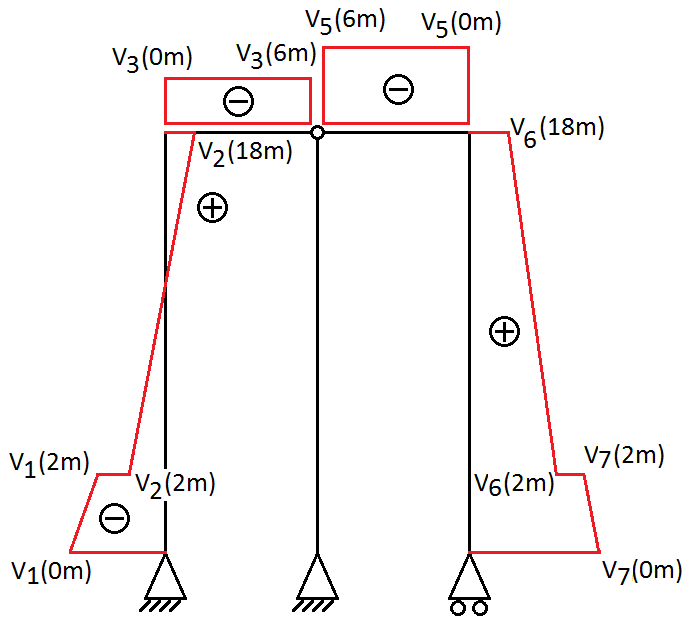
\includegraphics[width=0.7\textwidth]{billeder/sk.png}
	\caption{Forskydningskurve}
	\label{fig:forskydningskurve}
\end{figure}

\begin{figure}[H]
	\centering
	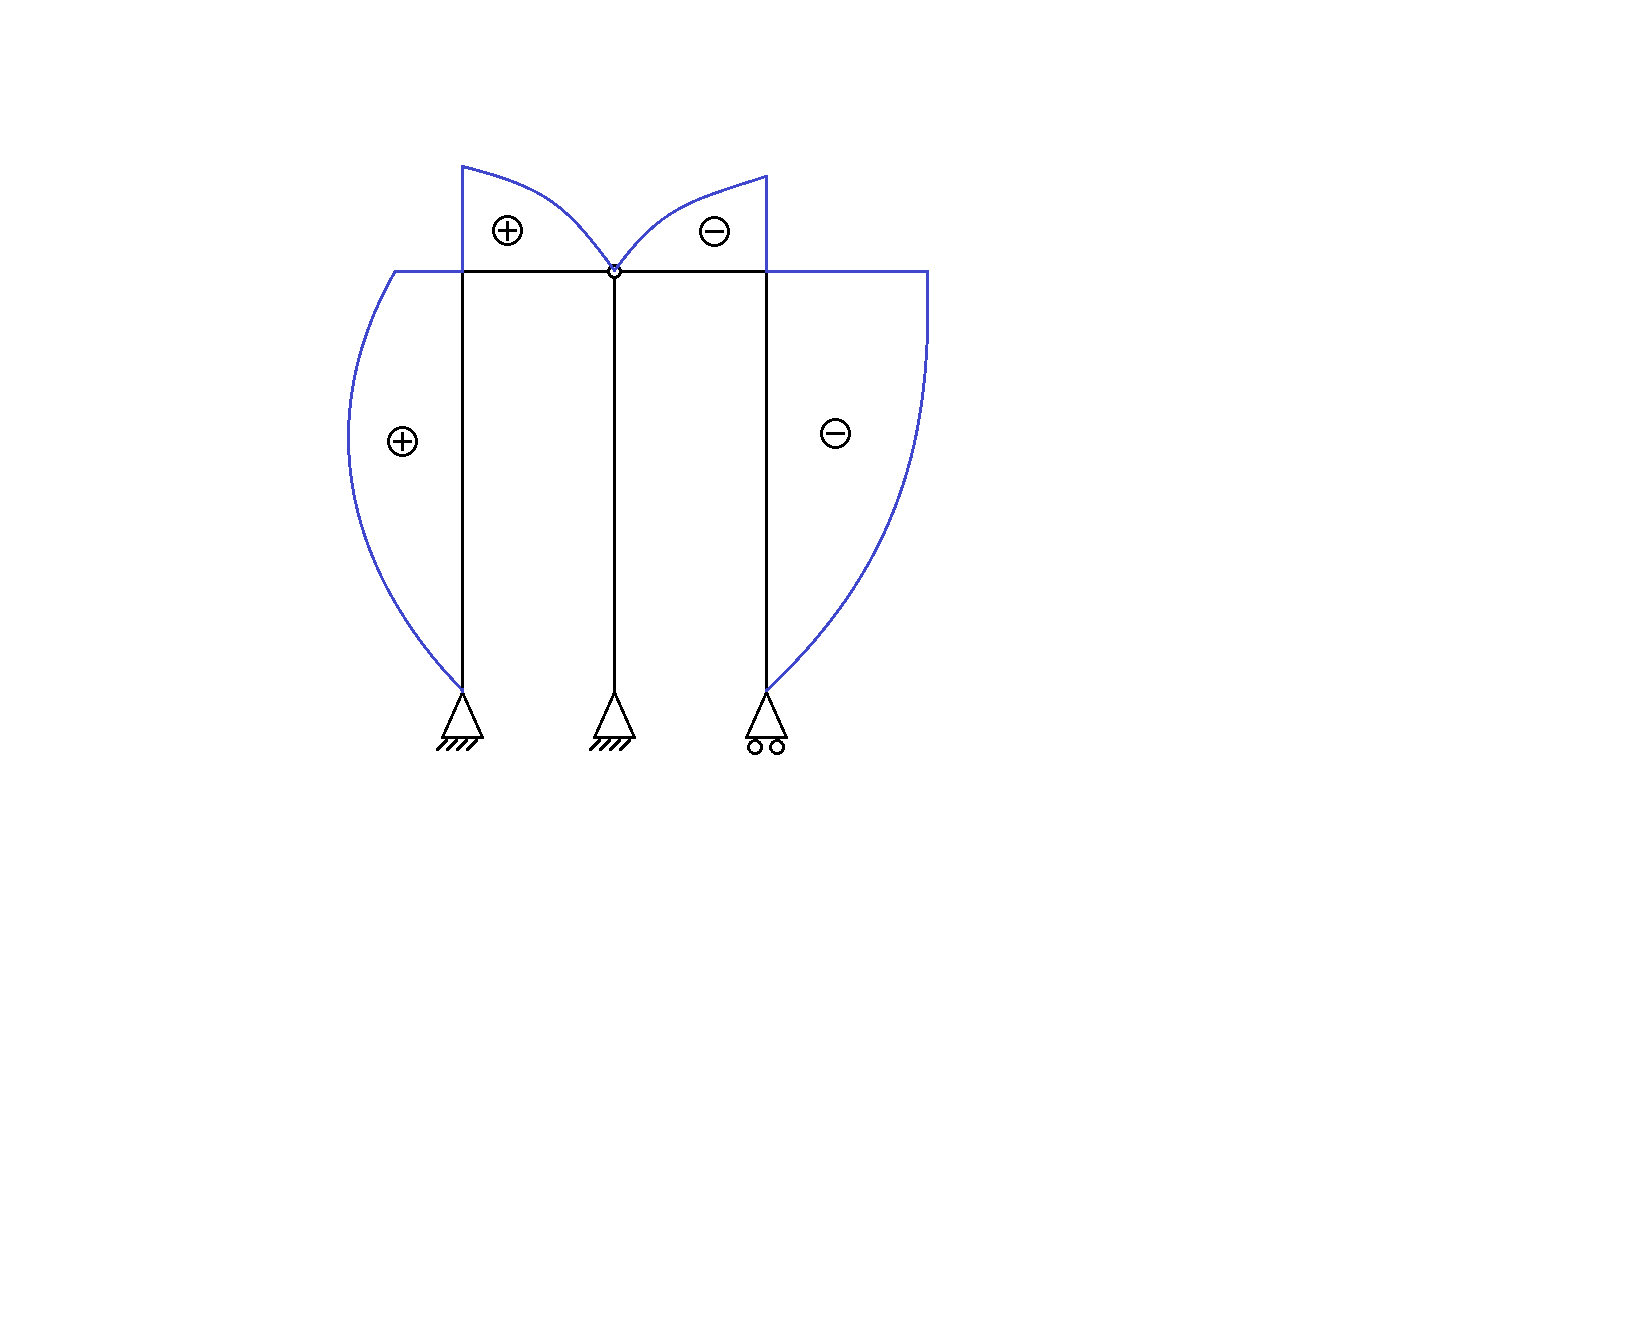
\includegraphics[width=0.7\textwidth]{billeder/skkm.png}
	\caption{Momentkurve}
	\label{fig:momentkurve}
\end{figure}

\begin{figure}[H]
	\centering
	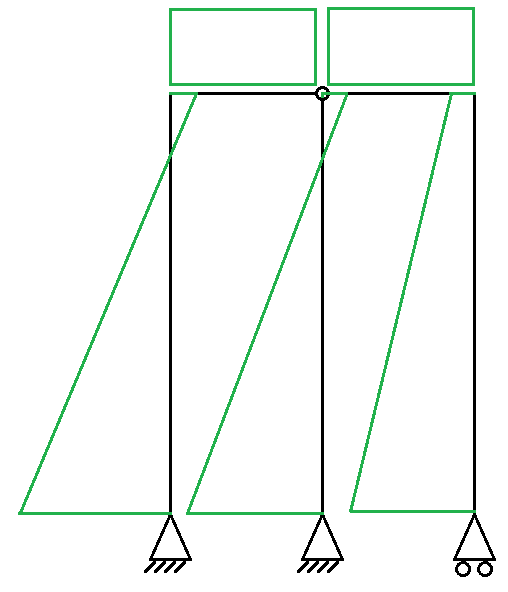
\includegraphics[width=0.7\textwidth]{billeder/SKFN.png}
	\caption{Normalkraftkurve}
	\label{fig:normalkraftkurve}
\end{figure}

\section{Spænding}
For at finde ud af om konstruktionen kan holde, undersøges spændingstilstanden. Her skal det gælde:

\begin{center}
	$\sqrt{\sigma^2 + 3\tau^2} \le f_y$ 
\end{center}

\begin{itemize}
	\item[-] $\sigma$: Normalspænding [MPa]
	\item[-] $\tau$: Forskydningsspænding [MPa]
	\item[-] $f_y$: Flydespænding [MPa]
\end{itemize}

Flydespændingen beregnes ved formlen:

\begin{center}
	$f_y = \frac{f_{yk}}{\gamma}$
\end{center}

\begin{itemize}
	\item[-] $f_{yk}$: Den karakteristiske flydespænding, der afhænger af ståltype. For ståltype S235 er $f_{yk} = 225 MPa$
	\item[-] $\gamma$: Partialkoefficient, der sættes til 1,1 \citep[ s. 212]{stabi}.  
\end{itemize}

Altså beregnes den regningsmæssige flydespænding til:

\begin{center}
	$f_y = \frac{225 MPa}{1,\!1} = 204,\!54 MPa$
\end{center}

Normalspændingen findes ved Naviers formel:

\begin{center}
	$\sigma = \frac{N}{A} - \frac{M}{I} y$
\end{center}

\begin{itemize}
	\item[-] N: Normalkraft [kN], som er bestemt igennem snitkræfter
	\item[-] A: Tværsnitsareal, som for stålprofil 450 er $14,\!7 \cdot 10^3 mm^2$ \citep{stabi}. 
	\item[-] M: Moment [kN], som er bestemt igennem snitkræfter
	\item[-] y: Tyngdepunktskoordinat [mm], som er $\pm 225$
	\item[-] I: Inertimoment, som for stålprofil 450 er $458,\!5 \cdot 10^6 mm^4$ \citep{stabi}. 
\end{itemize} 

Dernæst beregnes forskydningsspændingen ved Grasshofs formel:

\begin{center}
	$\tau = \frac{VQ}{Ib}$
\end{center}

\begin{itemize}
	\item[-] V: Forskydningskraft [kN], som er bestemt igennem snitkræfter
	\item[-] Q: 1. ordens arealmoment for $A_1$: $Q = \int_{A_1}y \mathrm{d}A = yA$ $[mm^3]$
	\item[-] b: bredde, som er 24,3 mm
\end{itemize}

Nedenfor vises et beregningseksempel for et kritisk punkt. Resultaterne for alle de valgte kritiske punkter kan ses på Figur \ref{fig:tabelspanding}. 
\newline
\newline
\textbf{Snit 5: Største forskydningskraft}
\newline
Normalspændingen og forskydningsspændingen beregnes begge ved henholdsvis $y = -225 mm$ og $y = 225 mm$, fordi I-profilens højde er 450 mm, og dermed er længden til y-koordinaten $\pm 225 mm$. Eksemplet nedenfor, er beregnet med $y = 225 mm$.

Først beregnes normalspændingen:
\begin{center}
	$\sigma = \frac{1,\!45 kN}{14,\!7 \cdot 10^3 mm^2} - \frac{-1011,\!72 kNm}{458,\!5 \cdot 10^6 mm^4} \cdot 225 mm = 496,\!58 MPa$
\end{center}

Dernæst beregnes forskydningsspændingen:
\begin{center}
	$\tau = \frac{-172,\!35 kN \cdot (225 mm \cdot 14,\!7\cdot10^3 mm^2)}{458,\!5\cdot10^6 mm^4 \cdot 24,\!3 mm} = -51,\!16 MPa$
\end{center}

Til sidst kan spændingstilstanden beregnes:
\begin{center}
	$\sqrt{496,\!58^2 MPa + 3 \cdot (-51,\!16)^2 MPa} = 504,\!43 MPa$
\end{center}

Denne spænding på 504,43 MPa, er for høj, idet flydespændingen er beregnet til $204,\!54 MPa$. Dermed vil konstruktionen bryde sammen.

 \begin{figure}[H]
 	\centering
 	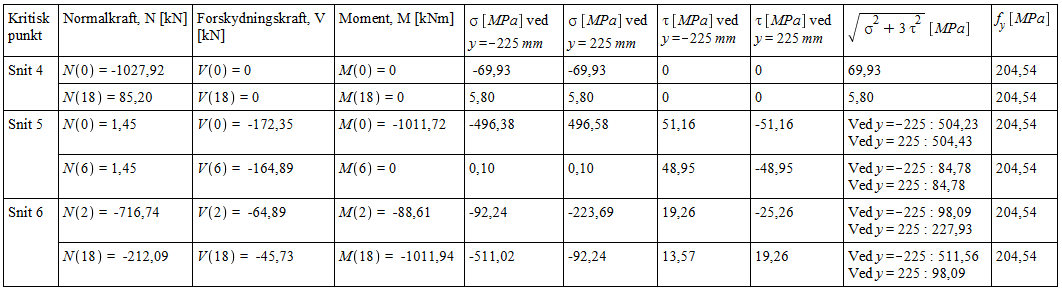
\includegraphics[width=1.1\textwidth]{billeder/tabelspanding.png}
 	\caption{Resultater af spændingstilstand}
 	\label{fig:tabelspanding}
 \end{figure}

Det ses på Figur \ref{fig:tabelspanding}, at spændingen i flere tilfælde overskrider den regningsmsæssige flydespænding. Derfor vil stålrammen opleve brud og i værste tilfælde knække sammen, som det kendes fra ståls arbejdskurve.
\newline 
\newline
For at konstruktionen ikke skal bryde sammen, skal der foretages en række ændringer.
\newline \indent{     }  Der er indsat tre stålrammer i tilbygningen. Ved at indsætte en eller to stålrammer mere, vil lasterne fordeles ud over disse, og dermed vil hver enkelt stålramme belastes mindre. Dermed vil spændingerne i sidste ende mindskes. 
\newline \indent{     }  Der er valgt en ståltype S235, som kan ændres til en højere styrkeklasse, for eksempel S275 eller S355. Ved at vælge en højere styrkeklasse, øges flydespændingen dermed. En større flydespænding betyder, at stålen kan klare en større spænding. Ved for eksempel kan ændre ståltypen til S355 ændres flydespændingen til $f_y = \frac{345 MPa}{1,\!1} = 313,\!64 MPa$. Dette er dog stadig ikke en stærk nok stål, og derfor kan dette ikke være den eneste ændring der skal foretages. 
\newline \indent{     }  Til sidst kan der vælges en anden stålprofil. Dette vil ændre henholdsvis højde, bredde, inertimomentet, densiteten, tværsnitsarealet, m.m. på stålprofilen. Dette vil give anledning til en mindre egenlast, hvis stålprofilen mindskes, og dermed en mindre spænding.
\newline
\newline
Helt så simpelt kan det dog ikke opstilles, da der for et rigtigt byggeprojekt også skal tages højde for det økonomiske aspekt af byggeriet, og omkostningerne. Hvis ikke leverandøren har en stærkere ståltype end S235 på lager, så kan omkostningerne hurtigt løbe op, når man er på udkig efter en stærkere type som eksempelvis S355, og det er derfor ikke muligt bare at vælge ståltype efter ønske, da det er omkostningsfuldt.
\chapter{Anvendelsesgrænsetilstand}
Nu er brudgrænsetilstanden bestemt, i det følgende regnes anvendelsesgrænsetilstanden. Ud fra anvendelsesgrænsetilstanden kan det vurderes, om bygningen har tilstrækkelig små deformationer til, at bygningens dimensioner kan godtages. 
\newline \indent{     }  Det antages, at der kun virker én variabel last på konstruktionen, nemlig vindlasten. Denne last forlænges helt ned til understøtningerne, og der ses bort fra jordlasten. Derfor er der udregnet nye reaktioner for konstruktionen, som ses i Tabel \ref{tab:anden}. Beregningerne kan ses i Bilag XX. 

\begin{table}
	\begin{center}
		\begin{tabular}{|c|c|c|}
			\hline
			Reaktion & Værdi & Enhed \\ \hline
			$S_x$ & -71,14 		& kN      \\ \hline
			$C_y$ & 578,86 		& kN      \\ \hline
			$S_y$ & 36,07 		& kN       \\ \hline
			$B_y$ & 1432,31 	& kN      \\ \hline
			$A_y$ & 344,53 		& kN      \\ \hline
			$B_x$ & 0,00 		& kN      \\ \hline
			$A_x$ & -147,87 	& kN       \\ \hline
		\end{tabular}
		\caption{Reaktioner for anvendelsesgrænsetilstand}
		\label{tab:anden}
	\end{center}
\end{table}

\section{Moment}
Der er lavet i alt fem snit på konstruktionen, som vist på Figur \ref{fig:snitanvendelse}. Dog ses der bort fra den højre del af konstruktionen, og dermed er det kun snit 1-3 der anvendes. 

\begin{figure}[H]
	\centering
	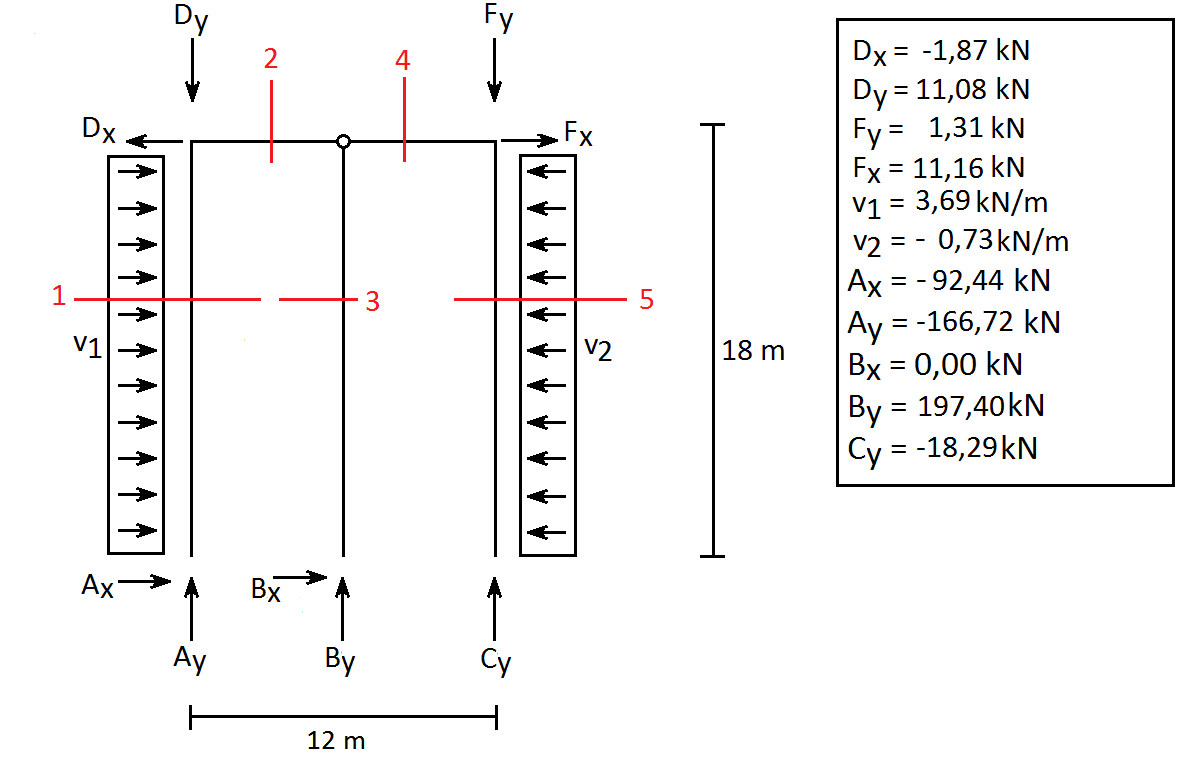
\includegraphics[width=0.9\textwidth]{billeder/snitanvendelse.png}
	\caption{Snit}
	\label{fig:snitanvendelse}
\end{figure}

Nedenfor er vist et eksempel på, hvordan momentligningen regnes for snit 1. Alle beregningerne findes i Bilag XX.
\newline
\newline
\textbf{Snit 1: 0 m < x < 18 m}
\newline
Fritlegemediagrammet for snit 1 ses på Figur \ref{fig:snitetan}.
\begin{figure}[H]
	\centering
	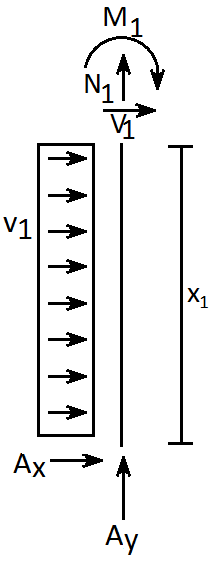
\includegraphics[width=0.2\textwidth]{billeder/asnitet.png}
	\caption{Snit 1}
	\label{fig:snitetan}
\end{figure}


Først bestemmes momentligningen for snit 1, 2 og 3 disse kaldes for $M_1$, $M_2$ og $M_3$:
\begin{equation}
M_1(x_1)=\frac{A_xx_1-\frac{1}{2}V_1x_1^2}{EI}
\end{equation}

\begin{equation}
M_2(x_2)=\frac{-\frac{1}{2}E_sx_2^2-E_1*18m*x_2-P_1_y*x_2+A_y*x_2-A_x*18m-V_1*162m^2}{EI}
\end{equation}

\begin{equation}
M_3(x_3)=\frac{B_x*x_3}{EI}
\end{equation}

\section{Bjælkens differentialligning}
For at udregne udbøjningerne for stængerne, anvendes bjælkens differentialligning. Da det statiske system for tilbygningen til Strøybergs Palæ er statisk bestemt, er det den anden ordens afledede, som anvendes for at bestemme udbøjningerne.
\newline

Først findes den første og anden aflede for $M_1$: 

Først findes den første og anden aflede for $M_1$: %Her vises integration%

 
\begin{equation}
	\int M_1(x_1) = \int \frac{- A_x\cdot x_1 - \frac{1}{2}\cdot V_1 \cdot x_1^2}{EI}
	= \alpha_1(x_1) = \frac{-\frac{1}{2} A_x x_1^2 - \frac{1}{6}  V_1  x_1^3 }{EI}
\end{equation}

\begin{equation}
	\int \alpha_1(x_1) = \int \frac{-\frac{1}{2} A_x x_1^2 - \frac{1}{6}  V_1  x_1^3 }{EI}
	= u_1(x_1) = \frac{1}{6} A_x x_1^3 - \frac{1}{24}  V_1  x_1^4 }{EI} + k_1 x_1 + k_2
\end{equation}

Samme metode bruges på de næste 2 momentligninger og det giver følgende udgangspunkt: 
\newline
$M_2$:
\begin{equation}
M_2(x_2) = \frac{- \frac{1}{2}E_s x_2^29 - E_1 \cdot 18m x_2 - P_ly x_2^2 + A_y x_2 - A_x \cdot 18m - V_1 \cdot (162m)^2 {EI}
	\end{equation}
	
	\begin{equation}
	\alpha_2(x_2) = \frac{-\frac{1}{6}E_s x_2^3 - E_1 \cdot 9m x_2^2 - \frac{1}{2} P_ly x_2^2 + \frac{1}{2} A_y x_2^2 - A_x \cdot 18m x_2 - V_1 \cdot (162m)^2 x_2 }{EI}
	\end{equation}
	
	\begin{equation}
	u_2(x_2) = \frac{-\frac{1}{24}E_s x_2^4 - E_1 \cdot 3m x_2^3 - \frac{1}{6} P_ly x_2^3 + \frac{1}{6} A_y x_2^3 - A_x \cdot 9m x_2^2 - V_1 \cdot (81m)^2 x_2^2 }{EI
	\end{equation} 
$M_3$:
\begin{equation}
M_3(x_3 = B_x x_3)
\end{equation}

\begin{equation}
\alpha_3 (x_3) \frac{1}{2}\frac{B_x x_3^2}{EI} + k_5
\end{equation}

\begin{equation}
u_3(x_3) = \frac{1}{6} \frac{B_x x_3^3}{EI} + k_5 x_3 + k_6
\end{equation}

Ved integrering af ligningningerne giver dette 6 ligningner med 6 ubekænkte konstanter. Dette kan løses ved at opstille 6 randbetingelser som er: 

\begin{table}[h]
	\begin{tabular}{l}
		$u\_1(0)=0       \\
		\alpha_1(h)=\alpha\_2(0) \\
		u\_1(h)=u\_3(h) \\
		u\_2(h)=0       \\
		u\_2(l)=0      $ \\
		
	\end{tabular}
\end{table}

De opsatte randbetingelser regnes ud og følgende 6 konstanter får værdierne: 

\begin{table}[h]
	\begin{tabular}{|c|c|}
		\hline
		k\_1=                       & -0.22                      \\ \hline
		k\_2=                       & 0                          \\ \hline
		k\_3=                       & -0.035                     \\ \hline
		k\_4=                       & 0                          \\ \hline
		\multicolumn{1}{|l|}{k\_5=} & \multicolumn{1}{l|}{-0.15} \\ \hline
		\multicolumn{1}{|l|}{k\_6=} & 0                          \\ \hline
	\end{tabular}
\end{table}

Konstanterne for den anden aflede af $M_1$ indsættes i ligningen og kurven udregnes. Dernæst findes den maksimale udbøjning, det gøres også for $M_2$ og $M_3$ og følgende 3 maksimale udbøjninger fåes: 

Konstanterne for den anden aflede af $M_1$ indsættes i ligningen og kurven udregnes. Dernæst findes den maksimale udbøjning, det gøres også for den anden aflede af $M_2$ og $M_3$ og følgende 3 maksimale udbøjninger fåes: 


%Tegning af udbøjning% 

Konklusion
\chapter{Geologi}
For at kunne dimensionere et fundament, er det vigtigt at have en grundlæggende viden om det materiale, der arbejdes med, altså hvilken jord, samt dets egenskaber og geologien i området. I det følgende vil der derfor foretages en beskrivelse af Aalborgs geologi, samt en beskrivelse af jorden og dets styrkeparametre.

\section{Jord}
\subsection{Beskrivelse af jord og jordtyper}
Jord er en massebetegnelse, da der findes mange forskellige typer af jordarter. Der findes to hovedgrupper af jord; rene mineraljordarter og organiske jordarter. 
\newline \indent{     }  De rene mineraljordarter kan være sorterede eller usorterede. Mineraljordarterne kan blive sorteret ved vand- og vindaflejring, og kan blive til det, der kendes som grus, sand, silt og ler. De usorterede mineraljordarter aflejres primært ved gletsjeraflejring, og betegnes som morænejordarter kaldet till.\citep{jordarter}
\newline \indent{     }  Organiske jordarter består af organisk materiale i form af plante- eller dyrerester. Disse jordarter kendes som muld, tørv, gytje mm.\citep{miljo}
\newline \indent{     } De forskellige jordtyper kan opdeles i to kategorier; friktionsjord og kohæsionsjord som har forskellige egenskaber. Egenskaberne afhænger af kornstørrelserne, som angives ved kornets diameter, og herved kan de inddeles i kornfraktioner\citep{geoteknik}.De grovkornede jordarter er friktionsjord hvor styrken kommer fra friktion mellem kornene. De finkornede jordarter er kohæsionsjord, hvor styrken skyldes indre sammenhæng mellem kornene.For eksempel ses inddelingen af kornstørrelserne for nogle mineral jordarter på Figur \ref{fig:kornstorrelser} .

\begin{figure}[htbp] \centering
	\begin{minipage}[b]{0.48\textwidth}\centering
		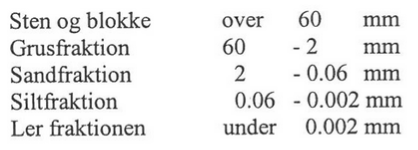
\includegraphics[width=1.0\textwidth]{billeder/kornetsdiameter.png}
		\caption{Inddeling af kornstørrelser for mineraljordarter (KILDE)}
		\label{fig:kornstorrelser}
	\end{minipage}\hfill
\end{figure}

\subsection{Jordtypernes udseende og dannelse}
Grus-  og sandjordarter skabes ved forvitring og erosion af materiale fra faste bjergarter. Materialet bliver herefter transporteret og aflejret via vind eller vand. Dette gør, at deres sammensætning bestemmes af udgangsmaterialet, men i lige så høj grad af transportmåden og transporttiden. Transporttiden kan gøre, at bløde dele af materialet opløses, samt at materialet får en afrundet kornform, og dette giver en mindre friktionsvinkel. Den relative store kornstørrelse ved grus og sandjordarter gør, at de har et groft porenet, hvilket medvirker, at vandet bevæger sig let i materialet,  dvs. at permeabiliteten er stor. Samtidig ved belastning af materialet sker der en vandudpresning, hvilket er en hurtig konsolidering.\citep{jordarter}
\newline \indent{     }  Grus- og sandjordarters styrkeegenskaber afhænger af friktionen mellem kornene, som afhænger af kornenes lejringstæthed, materialets enskornethed og kornenes enkelte form; om de er skarpkantet eller afrundet.\citep{jordarter} 
\newline \indent{     }  Lerjordarter har alle et bestemt indhold af lermineraler. Indholdet af disse har en betydende indflydelse på lerjordartens egenskaber, også selvom de ikke udgør størstedelen af jordarten. Lermineralerne bliver til ved en kemisk forvitring af faste bjergarter. De mest betydende grupper af lermineraler er; kaolinit, smectit, illit og chlorit. Den kemiske sammensætning af lermineralerne kan være meget forskellige og har en stor betydning for de fysiske egenskaber.\citep{jordarter} Alle lermineralerne kan optage vandmolekyler, hvilket gør, at lerjordarter kan indeholde meget vand. Betydningen af vandet kan fysisk ses ved tilsætning af vand til lerjordarterne, som gør at de sveller og ligeledes svinder ved tørring. Hvis lerpartiklerne er placeret med kort afstand til hinanden, vil dette give jordarten en større styrke.\citep{jordarter}  Ved at smadre jordarten formindskes jordartens styrke, men en del af denne styrke kan jordarten genvinde. \citep{jordarter}
\newline \indent{     }  Morænejordarter er typisk usorterede mineraljordarter, og kan derfor bestå af flere forskellige kornstørrelser. Fordelingen af dem kan skifte inden for korte afstande. Morænejordarter har normalt gode styrke- og deformationsegenskaber, da de er forbelastede.\citep{jordarter}
\newline \indent{     }  Organiske jordarters egenskaber er afhængige af de organiske bestanddeles art. De forskellige typer af organiske jordarter bliver dannet forskellige steder. Tørv og gytje bliver for eksempel dannet i moser, søer, bugter, fjorde mm, og dets styrke er ikke høj. Dette skyldes, at disse indeholder store mængder vand, da der ikke er faste partikler og at organiske materialer forsvinder med tiden. \citep{jordarter}

\subsection{Jords styrke og stivhed}
Jord betragtes, ligesom beton og stål osv, som et byggemateriale, da dens fysiske egenskaber er vigtige for konstruktions dimensionering.\citep{DGF} 
\newline \indent{     }  Jordarterne har meget forskellige styrker, og inden for geoteknik kan jordarterne inddeles i to forskellige typer. Den ene type er friktionsjord, for eksempel sand og grus. Den anden er kohæsionsjord med et indhold af mere end 10\% lerfraktion. 
Friktionsjord er under stabil lejring næsten usammentrykkeligt, og hvis deformationer finder sted forskydninger eller gnidninger kornene imellem.\citep{DGF}
\newline \indent{     }  I kohæsionsjord kan kornskelettet være stabilt ved åbne strukturer, men kun ved små deformationer og belastninger, afhængig af forbelastning. Ved store belastninger er disse jordarter sammentrykkelige.
\newline \indent{     }  Med hensyn til jordarters styrke, benyttes begreberne træk- og trykstyrke normalvis ikke. I stedet anvendes forskydningsstyrken. Denne anvendes da der ved brud i jorden, sker en forskydning af jordmasser. Når der sker et sådant brud, virker der normal- og forskydningsspændinger langs brudlinjen.\citep{geoteknik} Forskydningsspændingen $\tau_f$ virker som en reaktion på jordmassens bevægelse nedad, og derfor er denne rettet skråt op ad. Normalspændingen $\sigma_f$, også kaldet brudspændingen, står vinkelret på brudlinjen, og regnes positiv ved tryk \citep{geoteknik}. Dette er illustreret på Figur \ref{fig:poretrykket}. 

\begin{figure}[htbp] \centering
	\begin{minipage}[b]{0.48\textwidth}\centering
		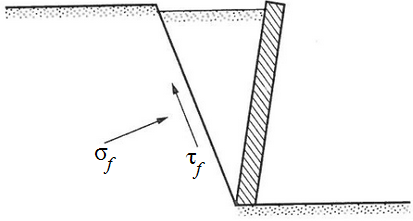
\includegraphics[width=1.0\textwidth]{billeder/poretrykket.png}
		\caption{BILLEDTEKST}
		\label{fig:poretrykket}
	\end{minipage}\hfill
\end{figure}

For at finde styrken i jord laves et triakselforsøg, der laves via et triaksialapparat, dette er illustreret på Figur \ref{fig:forskudningsspanding}. Forsøget er det mest anvendte for at finde jords styrke. En cylindrisk jordprøve tilpasses så den har samme diameter som højde. Prøven indsættes lodret i apparatet og indesluttes en tæt gummimembran. Trykhoveder er placeret på prøvens ender, disse er gjort næsten helt glatte vha. siliconesmurte gummihinder, der gør det muligt at holde prøvens cylindriske form indtil bruddet.  
\newline \indent{     } Forsøget kan deles op i to faser kaldet 1. isotrop spændingstilstand, 2. Voksende deviatorspæning. Begge faser kan gennemføres på to forskellige måder. Fase 1 hvor kammertrykket indstilles som ønsket, gennemføres konsolideret eller ukonsolideret, hvor drænventilerne er åben i den konsolideretproces og lukket i den ukonsolideret. I fase 2. påføres prøven gradvist et øget stempeltryk, hvor der til sidst sker et brud i prøven. Denne fase kan også udføres med lukket eller åben ventil, og kaldes for henholdsvis drænet og udrænet \citep{geoteknik}.
\begin{figure}[htbp] \centering
	\begin{minipage}[b]{0.48\textwidth}\centering
		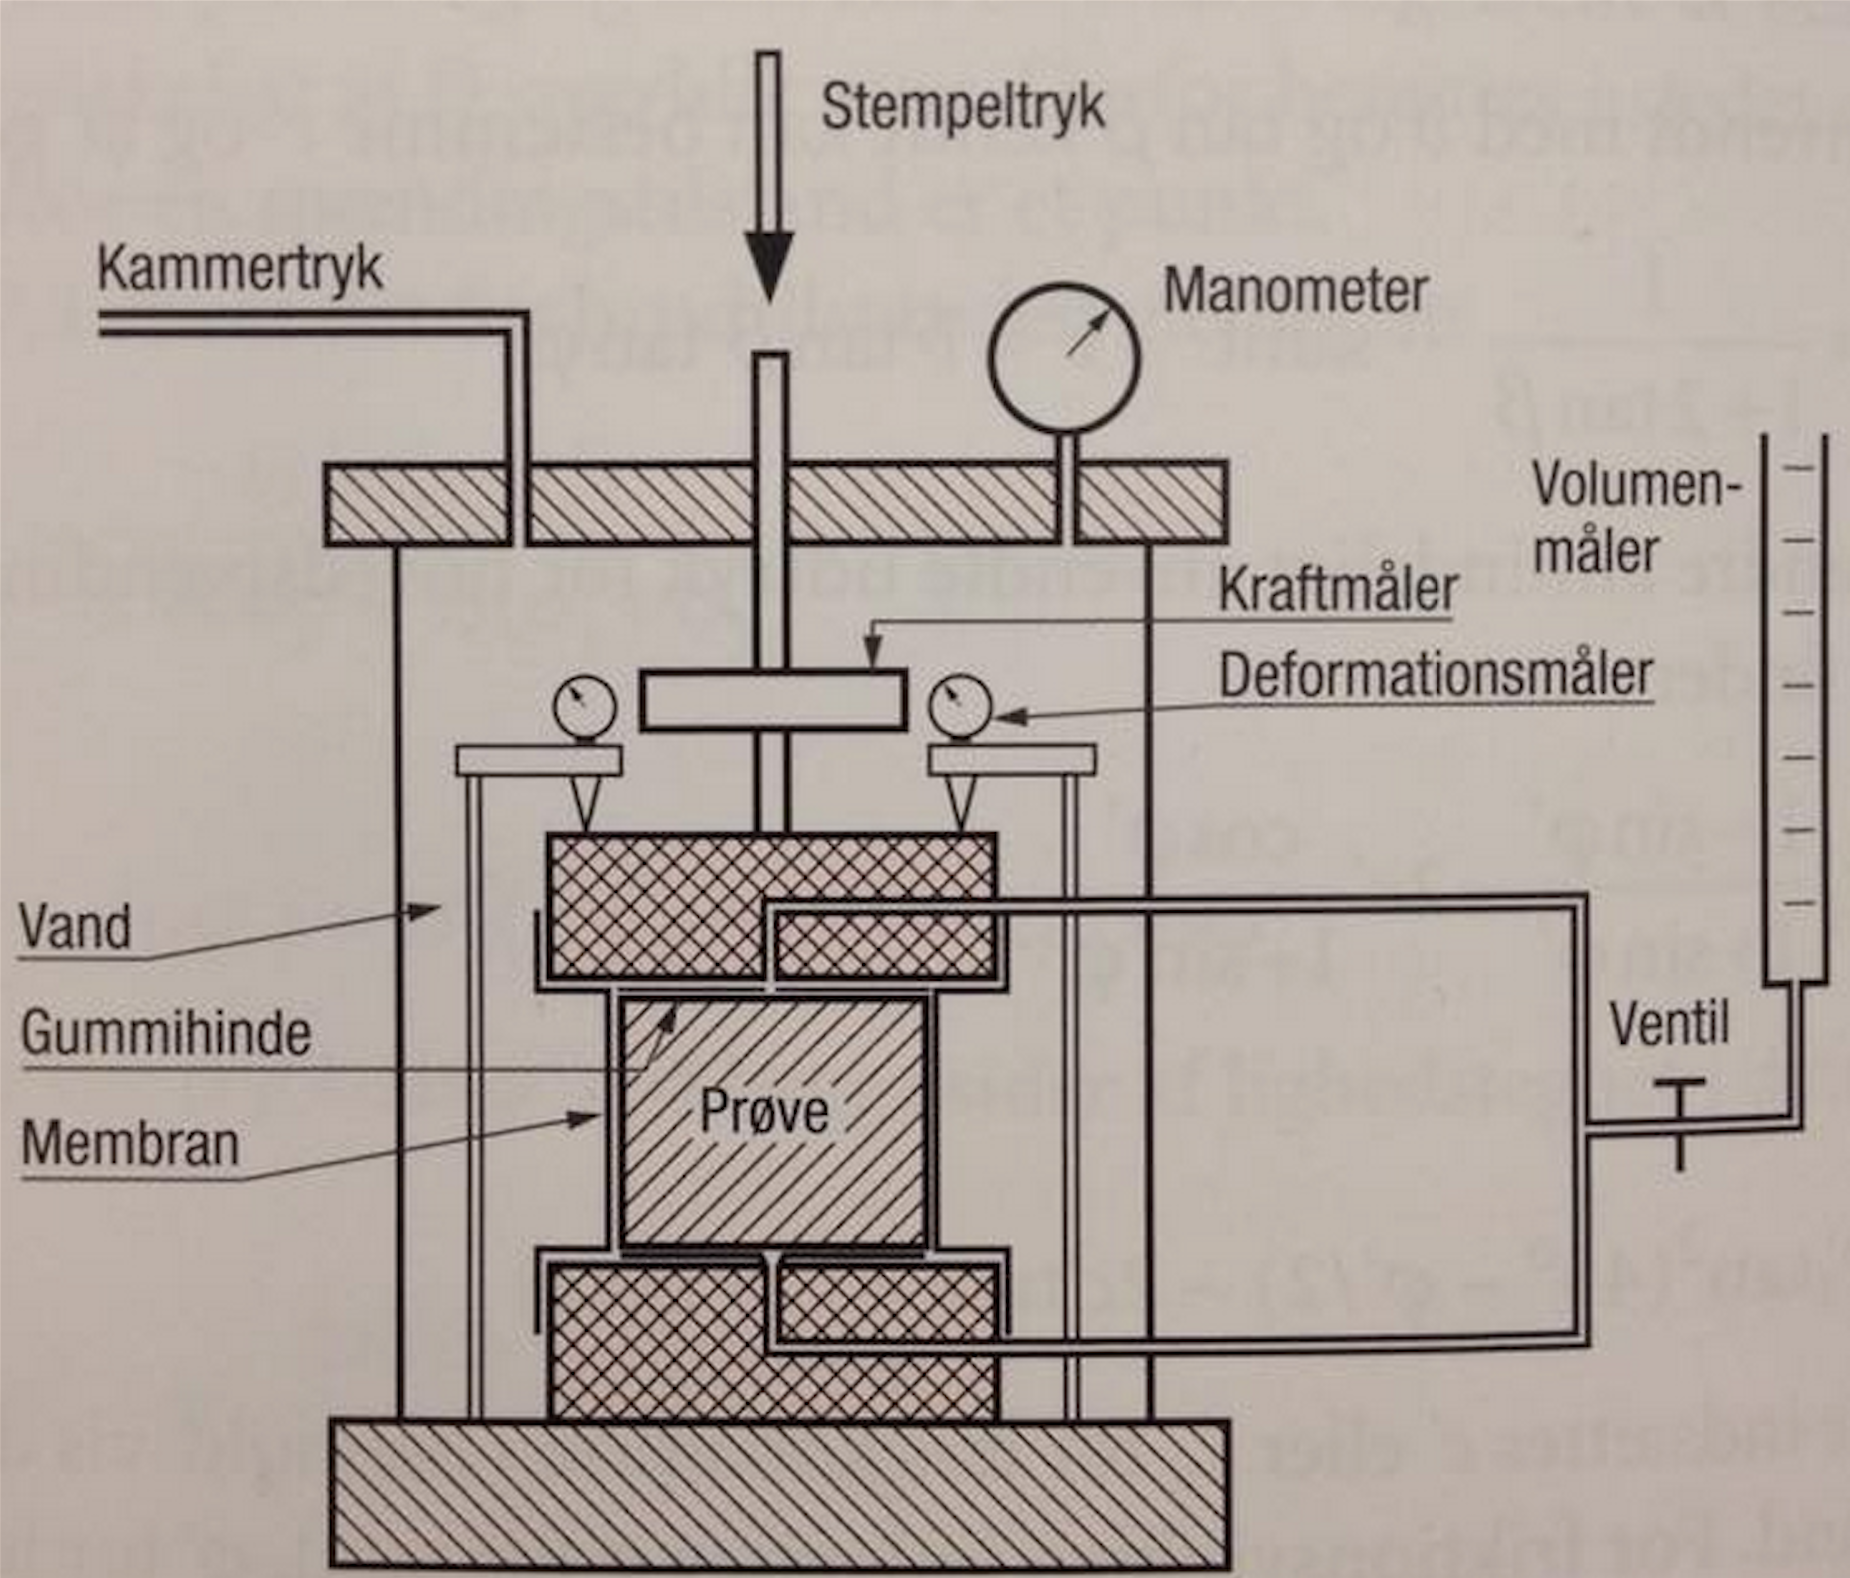
\includegraphics[width=0.8\textwidth]{billeder/forskud.png}
		\caption{BILLEDTEKST}
		\label{fig:forskudningsspanding}
	\end{minipage}\hfill
\end{figure}

\indent{     } 																																																																																																																																																																																						 Friktionsvinklen er et mål for jord styrke. Friktionsvinklen er vidt forskellige alt efter jordtype, hvilket er illustreret på Figur \ref{fig:friktionsvinkler}. Spændingernes størrelse har en betydning, da friktionsvinklen aftager med voksende spændinger. Der optræder også en kohæsion med disse spændinger, men dette er svært at regne i praksis, og derfor sættes c (kohæsion) oftest lig nul ved eksempelvis sand. 

\begin{figure}[htbp] \centering
	\begin{minipage}[b]{0.48\textwidth}\centering
		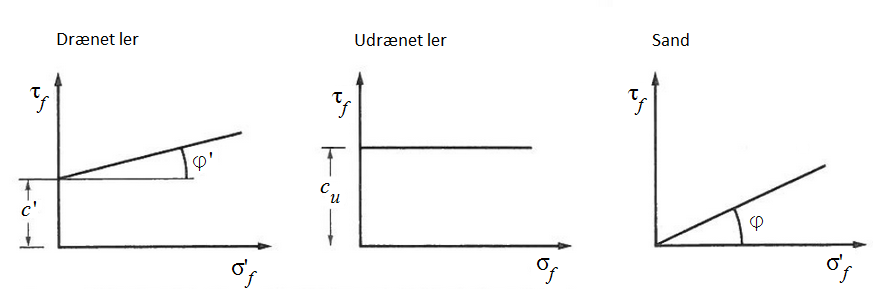
\includegraphics[width=1.0\textwidth]{billeder/friktionsvinkeller.png}
		\caption{Brudbetingelser for ler og sand \citep{geoteknik}}
		\label{fig:friktionsvinkler}
	\end{minipage}\hfill
\end{figure}

\section{Aalborgs geologi}
Det danske landskab er overvejende formet under den sidste istid, Weichselistiden, der fandt sted for ca. 114.000-10.000 år siden. Under jordoverfladen findes bjergarter og aflejringer fra tidligere end Weichselistiden. Det ældste i Danmarks dybder er grundfjeldet, bestående af granit og gnejs \citep{geopdf}, der anses for at ligge som en sokkel under Danmark og regnes for at være 1.200-850 mio. år gammel. Over grundfjeldet findes aflejringer, der viser, hvordan klima, flora, fauna og jordskorpen har ændret sig de sidste ca. 500 mio. år samt hvordan hav og land skiftevis har haft indflydelse på området \citep{geolink}.
\newline
\newline
Kridttiden startede for 135 mio. år siden og sluttede igen for 65 mio. år siden. Kridttiden er opdelt i to perioder; Nedre- og Øvre Kridt, hvor Nedre Kridt strækker sig fra 135-100 mio. år siden, mens Øvre Kridt er fra 100-65 mio. år siden.  Øvre Kridt består hovedsageligt af skrivekridt \citep{geopdf}, som er en hvid bjergart, der let smitter af og indeholder store mængder kalk, ofte mellem 95 og 99,5\%. Kridtlagene er afsat på bunden af havet, som formodes at have haft en vanddybde på 100-250 m. Ved kridtlagets overflade findes såkaldte skorstene, der er skrå eller lodrette rør, ned gennem kridtlaget, fyldt med jord \citep[ s. 15-16]{geobog}. Kridtlaget varierer i Danmark fra en tykkelse på 500 m til 2000 m.
\newline
\newline
Efter Kridttiden begyndte Tertiærtiden, der kan inddeles i flere underperioder, og som går fra år 65 mio. til 2,5 mio. før nu.
\newline \indent{     }  Danien, også kaldet Nedre Paleocæn, dækker fra 65-62 mio. år før nu og minder om Øvre Kridt, da Danien også består af forskellige slags kalksten og flint. Der er dog den forskel, at Danien også indeholder forstenede dyr, hvilket Øvre Kridt ikke gør. Selve tykkelsen af Danien varierer fra 100 m til lidt over 200 m.
\newline \indent{     }  Paleocæn dækker fra 62-55 mio. år siden. Dette lag indeholder meget ler, hvilket giver sedimenttypen mergel, når leret og kalken blandes. Øverst i Paleocæn befinder sig et lag af kalkfrit ler. Tykkelsen af Paleocæn for Danmark er vidt forskellig, men størst tykkelse findes på Midtsjælland, hvor der er 160 m.
\newline \indent{     }  Imellem Nedre Paleocæn og Paleocæn findes et lag af bjergarten grønsandskalk, der er kalkrig, sandt og glauconitholdig.
\newline \indent{     }  Eocæn starter i år 55 mio. år før nu og slutter 38 mio. før nu. Skellet fra Paleocæn og Eocæn består i et vulkanudbrud syd fra Norges sydkyst. Vulkanudbrudet afspejles i askelagene, som der findes 180 af, der tydeligt ses som mørke lag i det lyse moler, der består af ler og kiselskaller af encellede planter. Moleret er 50-60 m tyk for de vestlige egne af Limfjorden, mens den er 15 m tyk syd og sydøst for de vestlige egne af Limfjorden \citep{geopdf}.
\newline
\newline
Kvartærtiden omfatter de sidste 2,5 mio. år tilbage og til nu og er kendetegnet ved store klimasvingninger mellem kolde og varme perioder. Weichsel-istiden, som er den sidste kolde periode i Kvartærtiden hidtil, stoppede for ca. 22.000 år siden. Da Weichelisen forsvandt, var det meste af Danmarks nuværende landskab over havet. Undtaget var det nordligste af Jylland, hvor de smeltende gletcher skabte havstigning, som skyllede ind over området. Havet var et højarktisk ishav, som opstod da isen smeltede, og har fået navnet Yoldiahavet. I den sydlige og sydvestlige del af Vendsyssel blev Yoldiahavet afgrænset mod et aflejringsområde, der formodes at have været en stor smeltevandssø, hvori en skalfri leraflejring opstod. Denne leraflejring kaldes også for Aalborg ler og er en blød ler, der danner grundlag for Aalborgs geologi, som kun er mild komprimeret af isen. Først for ca. 13.000 år siden trak Yoldiahavet sig tilbage, efter at have lagt ind over Vendsyssel i godt 2.000 år. Yoldiahavet blev trukket tilbage, da landskabet hævede sig, efter at have været tynget af isen, der nu var smeltet bort \citep{geopdf}.

\section{Boreprofiler} 
I og med Aalborg har en undergrund primært bestående af Aalborgler, burde der anvendes pælefundering, men da der ønskes at arbejde med direkte fundering, tages der udgangspunkt i boreprofiler fra Hals, hvor undergrunden primært består af sand. Der ses på boring B17, som er vedlagt i Bilag XX. 
\newline \indent{     }  På boreprofil 17 ses, at grundvandsspejlet ligger omkring 0,8 m under overfladen. Der aflæses også, at undergrunden primært består af sand for boreprofilen. Via den stiplede linje aflæses vandindholdet i jordlaget, mens den anden linje, der ikke er stiplet, fortæller noget om komprimeringen af jorden, altså hvor meget modstand jorden har.
\newline \indent{     }  I boreprofil 16 i Bilag YY findes et lag gytje mellem kote 2 og 3. Det ses, at vandindholdet i gytje er højere, samtidig med at modstanden i jordlaget ikke er højt. Når der funderes, skal der tages højde for denne svaghed i gytje, hvor der i nogle tilfælde vælges at grave laget væk, hvis gytjen ikke ligger for langt nede. Da den valgte boreprofil 17 ikke indeholder et lag af gytje, kan projektgruppen med fordel lave en direkte fundering. 
\chapter{Dimensionering af fundament}
Nu hvor Aalborgs geologi er undersøgt og analyseret, kan der bestemmes en fundamentstype. I dette afsnit vil der blive fremlagt forsøg til videre beregninger af friktionsvinklen for sand, som er med til at bestemme fundamentsstørrelsen.  

Metatekst
\section{Fundering}
Et fundament er en del af et bygværk, hvor formålet er at overføre belastningen fra bygningen til underliggende, bærende jordlag. Der findes mange forskellige funderingsmetoder, for eksempel pælefundering og direkte fundering, og kan i nogle tilfælde kombineres. De to mest almindelige funderingsmetoder er pæle- og direkte fundering, hvilke vil blive omtalt i denne rapport.
\newline \indent{     }  Ved direkte fundering støbes fundamentet direkte på terrænet, hvor de bæredygtige jordlag findes relativt tæt under bygningen. Belastningen overføres fra bygningen til jorden igennem vandrette flader. Belastningen på fundamentfladen udgøres af fundamentets egenvægt og bygingens belastning. Hvis belastningen virker på en lang fundamentflade med konstant bredde, er der tale om et stribefundament, der som regel bruges ved fundering af bærende vægge. Modsætningen hertil er punktfundamenter, som er rektangulære eller kvadratiske, og disse bruges for eksempel ved fundering af master, søjler og skorstene \citep[ s. 221]{geoteknik}. Stribefundamentet og punktfundamentet er illustreret på Figur \ref{fig:fundament}. 

\begin{figure}[htbp] \centering
	\begin{minipage}[b]{0.48\textwidth}\centering
		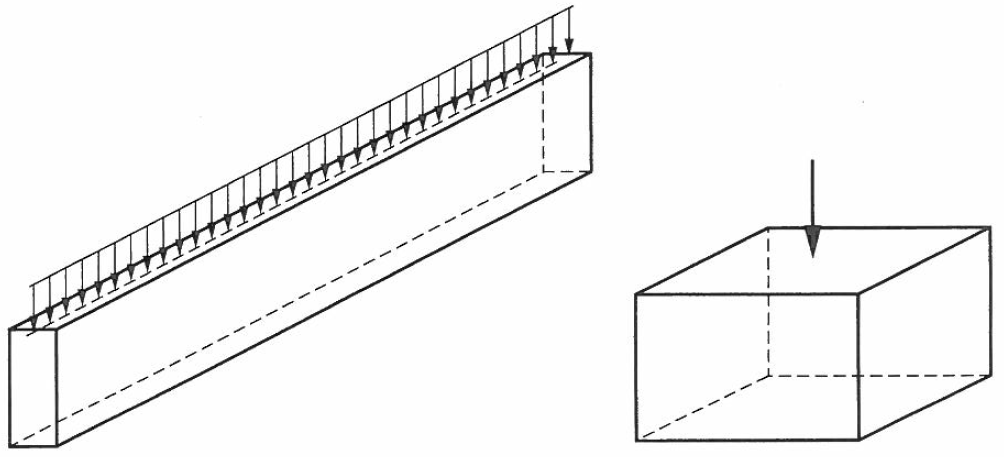
\includegraphics[width=1.0\textwidth]{billeder/fundament.png}
		\caption{Stribefundament og punktfundament \citep[ s. 221]{geoteknik}}
		\label{fig:fundament}
	\end{minipage}\hfill
\end{figure}

\indent{     }  Hvis de bæredygtige jordlag ligger mere end 4-5 meter under bygingen, anvendes ofte pælefundering. Ved pælefundering er søjleformede pæle af træ, beton, og/eller stål, rammet, presset, vibreret eller udstøbt i jorden. Pæleformen er normalt cylindrisk med cirkulært eller kvadratisk tværsnit. Pælefundering benyttes blandt andet når de bærende jordlag ligger så dybt, at direkte fundering vil blive uøkonomisk \citep[ s. 355]{geoteknik}.
\newline
\newline
Valg af funderingsmetode for tilbygningen til Strøybergs Palæ afhænger af jordbunds- og grundvandsforhold samt de belastninger, som konstruktionen er udsat for \citep[ s. 355]{geoteknik}. Det er derfor nødvendigt at have kendskab til områdets geologi omkring Strøybergs Palæ, og at tolke på de boreprofiler, der bliver udført på stedet, hvilket gøres i Afsnit 8.4. 

\section{Forsøg}
For at bestemme styrkeparametre for jorden udføres laboratorieforsøg, der bruges ved dimensionering af fundamentet. Forsøgene er udført på baskarpsand fra Sverige, hvilket antages at være sandet fra boreprofilerne.
\newline
\newline
Formålet med forsøgene er at bestemme friktionsvinklen, givet ved: 

\begin{equation}
	\varphi = 30^\circ - \frac{3}{U} + (14 - \frac{4}{U}) I_D
\end{equation}

\begin{itemize}
	\item[-] $U$: Uensformighedtal
	\item[-] $I_D$: Relativ lejringstæthed
\end{itemize}

Friktionsvinklen $\varphi$ er et mål for jords styrke, og skønnes ud fra sigteanalyse samt løs og fast lejring. Ved hjælp af nedenstående fire forsøg bestemmes friktionsvinklen, idét uensformighedstallet og den relative lejringstæthed bestemmes herudfra: 
\begin{enumerate}
	\item Vandindhold
	\item Sigteanalyse
	\item Kornvægtfylde
	\item Løs og fast lejring
\end{enumerate}
Tabeller over resultater, fremgangsmåde, apparaturliste samt fejlkilder for de enkelte forsøg findes i Bilag B-E.

\subsection{Forsøg 1: Vandindhold}
Formålet med forsøget er at finde vandindholdet \textit{w} i jordprøven. Vandindholdet er defineret som jordens vægttab i \% af tørvægten ved tørring i et varmeskab ved en temperatur på 105$^{\circ}$C. For naturligt forekommende jordarter kan vandindholdet ligge mellem nul og flere hundrede procent.
\newline
\newline
Vandindholdet beregnes ved:

\begin{equation}
	w = \frac{W_w}{W_s}\cdot 100\% = \frac{(W+sk)-(W_s+sk)}{(W_s+sk)-sk}\cdot 100\%
\end{equation}

\begin{itemize}
	\item[-] $W_w$: Vægten af vandet i prøven [g]
	\item[-] $W_s$: Vægten af det tørrede materiale [g]
	\item[-] $W$: Vægten af prøven før tørring [g]
	\item[-] $sk$: Vægten af skålen [g]
\end{itemize}

Forsøget er udført to gange. De fundne værdier for de to udførte forsøg ses i Tabel \ref{tab:bilaga1} i Bilag B. Vandindholdet for de to forsøg er beregnet til:
\begin{equation}
	\text{Forsøg 1}: w = \frac{81,\!02 \text{g} - 80,\!99 \text{g}}{80,\!99 \text{g} - 3,\!07 \text{g}}\cdot 100\% = 0,\!04\%
\end{equation}

\begin{equation}
	\text{Forsøg 2}: w = \frac{89,\!83 \text{g} - 89,\!79 \text{g}}{89,\!79 \text{g} - 3,\!11 \text{g}}\cdot 100\% = 0,\!05\%
\end{equation}

Ud fra de opnåede resultater, kan det konkluderes, at det benyttede materiale vurderes at være tørt og det meget lille vandindhold har ikke indflydelse på de øvrige resultater.
\newline \indent{     }  Til videre beregninger benyttes gennemsnittet for vandindholdet for forsøg 1 og forsøg 2, som er $0,\!04$\%. Dette skal bruges som et rent tal, som er $4 \cdot 10^4$. 

\subsection{Forsøg 2: Sigteanalyse}
Formålet med forsøget er at bestemme jordkornenes vægtmæssige fordeling efter størrelse i sand- og grusfraktion, for at beregne uensformighedstallet \textit{U} for jorden:
\begin{equation}
	U = \frac{d_{60}}{d_{10}}
\end{equation}

\begin{itemize}
	\item[-] $d_{60}$: 60\%-fraktilen
	\item[-] $d_{10}$: 10\%-fraktilen
\end{itemize}

Uensformighedstallet fortæller, hvor velsorteret jorden er:
\begin{itemize}
	\item[-] Velsorteret: $U < 2$
	\item[-] Sorteret: $2 < U < 3,\!5$
	\item[-] Ringe sorteret: $3,\!5 < U < 7$
	\item[-] Usorteret: $U > 7$
\end{itemize}

Forsøget er udført to gange, og der er derfor lavet en sigtekurve for hvert forsøg, og uensformighedstallet er udregnet for begge forsøg. 
\newline \indent{     }  Det procentvise gennemfald i hver sigte er beregnet, og herudfra fås sigtekurverne vist på Figur \ref{fig:sigtekurve1} og Figur \ref{fig:sigtekurve2}. Værdierne der er brugt til at finde det procentvise gennemfald på Figur \ref{fig:forsoget} og Figur \ref{forsogto} i Bilag C. 

\begin{figure}[htbp]
		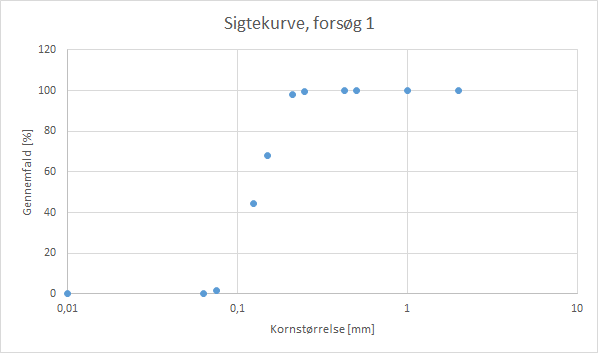
\includegraphics[width=1.0\textwidth]{billeder/sigtekurve1.png}
		\caption{Sigtekurve til forsøg 1}
		\label{fig:sigtekurve1}
\end{figure}

\begin{figure}[htbp]
		\centering
		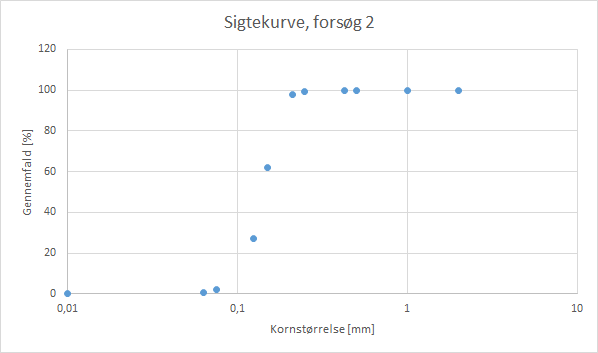
\includegraphics[width=1.0\textwidth]{billeder/sigtekurve2.png}
		\caption{Sigtekurve til forsøg 2}
		\label{fig:sigtekurve2}
\end{figure}

Uensformighedstallet for begge forsøg er beregnet, ved at lave lineær regression imellem henholdsvis 10\% og 60\% og derved finde 10\%-fraktilen og 60\%-fraktilen.
\newline
\newline
Ved det første udførte forsøg er 10\%-fraktilen fundet ved at lave lineær regression imellem sigte med maskestørrelse $0,\!075$ mm og $0,\!125$ mm, hvor følgende ligning fremgår: 
\begin{equation}
	y = 862,\!42x - 63,\!223
\end{equation}

For at finde 60\%-fraktilen er der lavet lineær regression imellem sigte med maskestørrelse $0,\!125$ mm og $0,\!15$ mm, hvor følgende ligning fremgår:
\begin{equation}
	d_{60}=937,\!12x - \SI{72,56}{mm}
\end{equation}

Ved forsøg 1 er 10\%-fraktilen og 60\%-fraktilen hermed beregnet til: 
\begin{equation}
	d_{10} = 0,\!08 \text{og} d_{60} = \SI{0,14}{mm}
\end{equation} 

Uensformighedstallet i forsøg 1 er derved:
\begin{equation}
	U = \frac{0,\!14}{0,\!08} = 1,\!67
\end{equation}

Ved forsøg 2 er 10\%-fraktilen, 60\%-fraktilen og uensformighedstallet beregnet til:
\begin{equation}
	d_{10} = 0,\!91 \text{og} d_{60} = 0,\!15$ \text{og} $U = \frac{0,\!15}{0,\!91} = 1,\!64
\end{equation} 
Uddybbende beregninger er vist i Bilag C.

Til videre beregninger benyttes gennemsnittet af uensformighedstallet for forsøg 1 og forsøg 2, som er $1,\!65$. Dette tal fortæller, at jorden er velsorteret, idet $U<2$. Dette stemmer godt overens med de observationer der forinden forsøget var gjort af sandet, hvor blev vurderet til at være ens- og afrundede korn. 

\subsection{Forsøg 3: Kornvægtfylde}
Formålet med forsøget er at finde den relative densitet $d_s$, også kaldet kornvægtfylden, for jordprøven. For jordarter uden organisk indhold kan kornvægtfylden variere fra $2,\!65$ for rent kvartsand til $2,\!85$ for visse lermineraler. I dette forsøg søges altså et resultat der ligger så tæt på $2,\!65$ som muligt.
\newline
\newline
Kornvægtfylden beregnes ved:

\begin{center}
	$d_s = \frac{W_s \rho_w^t}{(W_s + W_2 - W_1)\rho_w^{4^{\circ}}}$
\end{center}

\begin{itemize}
	\item[-] $W_s$: Vægten af tørt kornmateriale [g]
	\item[-] $p_w^t$: Densitet af luftfrit demineraliseret vand ved målte temperatur $[\frac{g}{cm^3}]$
	\item[-] $W_2$: Vægten af pyknometeret fyldt med luftfrit demineraliseret vand [g]
	\item[-] $W_1$: Vægten af pyknometer fyldt med prøve og luftfrit demineraliseret vand [g]
	\item[-] $\rho_w^{4^{\circ}}$: Densitet af luftfrit demineraliseret vand ved $4^{\circ}$, som er $1 \frac{g}{cm^3}$
\end{itemize}

Forsøget er udført to gange, og resultater for de to forsøg kan ses i Tabel \ref{tab:bilagc1} Bilag C. Kornvægtfylden for de to forsøg er beregnet til:

\begin{center}
	Forsøg 1: $d_{s} = \frac{161,\!27 g \cdot 0,\!998 \frac{g}{cm^3}}{(161,\!27 g + 641,\!16 g - 728,\!89 g)\cdot 1 \frac{g}{cm^3}} = 2,\!19$
\end{center}
\begin{center}
	Forsøg 2: $d_{s} = \frac{150,\!06 g \cdot 0,\!998 \frac{g}{cm^3}}{(150,\!06 g + 615,\!97 g - 709,\!40 g)\cdot 1 \frac{g}{cm^3}} = 2,\!64$
\end{center} 

Resultatet fra forsøg 2 anvendes til videre beregninger, fordi resultatet fra forsøg 1 vurderes til at være for langt fra den ønskede værdi på $2,\!65$. Grunden til den store afvigelse kan skyldes, at der blev anvendt ca. 161 g i forhold til, at der kun skulle være anvendt 150 g.

\subsection{Forsøg 4: Løs og fast lejring}
Formålet med forsøget er at finde jordens relative lejringstæthed $I_D$. Lejringstætheden er et tal, som vokser fra 0 til 1, når lejringstætheden varierer fra den løseste til den fasteste lejring.
\newline
\newline
$I_D$ bestemmes ved:

\begin{center}
	$I_D = \frac{e_{max} - e_{in situ}}{e_{max} - e_{min}}$
\end{center}

\begin{itemize}
	\item[-] $e_{min}$: jordens gennemsnitlige poretal for den fasteste lejring 
	\item[-] $e_{max}$: jordens gennemsnitlige poretal for den løseste lejring
	\item[-] $e_{in situ}$: jordens naturlige poretal 
\end{itemize}

Poretallet \textit{e}, for henholdsvis den løseste og fasteste lejring beregnes ved:

\begin{center}
	$e = \frac{d_s \rho_w  V}{W_s} - 1$
\end{center}

\begin{itemize}
	\item[-] $d_s$: kornvægtfylde [rent tal], som er fundet i forsøg 3: kornvægtfylde, til $2,\!64$ 
	\item[-] $\rho_w$: Vands densitet på $1 \frac{g}{cm^3}$
	\item[-] V: Volumen af materialet $[cm^3]$
	\item[-] $W_s$: Vægten at tørt kornmateriale [g]
\end{itemize}
 
Der er udført fire forsøg for henholdsvis den løseste og den fasteste lejring. Resultater samt poretallet for hvert enkelt forsøg ses i Tabel \ref{tab:bilagd1} og Tabel \ref{tab:bilagd2} i Bilag D.
Det gennemsnitlige poretal er:

\begin{center}
	$e_{min} = \frac{0,\!595 + 0,\!571 + 0,\!573 + 0,\!569}{4} = 0,\!577$
\end{center}

\begin{center}
	$e_{max} = \frac{0,\!873 + 0,\!875 + 0,\!874 + 0,\!873}{4} = 0,\!874$
\end{center}

Herefter bestemmes jordens naturlige poretal $e_{in situ}$ ved:

\begin{center}
	$e_{in situ} = (1 + w) \frac{d_s  \rho_w  V}{W_s} - 1$
\end{center}

\begin{itemize}
	\item[-] w: det naturlige vandindhold [rent tal], fra forsøg 1: vandindhold, til $0,\!0004$ 
\end{itemize}

Dette er beregnet til:

\begin{center}
	$e_{in situ} = (1+0,\!0004) \cdot \frac{2,\!64 \cdot 1,\!00 \frac{g}{cm^3} \cdot 269,\!39 cm^3}{421,\!4 g} - 1 = 0,\!691$
\end{center}

Slutteligt kan den relative lejringstæthed $I_D$ bestemmes til:

\begin{center}
	$I_D = \frac{0,\!874 - 0,\!691}{0,\!874 - 0,\!577} = 0,\!617$
\end{center}

\subsection{Friktionsvinklen}
Efter udførelsen af de fire forsøg kan friktionsvinklen beregnes til:

\begin{center}
	$\varphi = 30^\circ - \frac{3}{1,\!65} + (14 - \frac{4}{1,\!65}) \cdot 0,\!619 = 35,\!3^\circ$
\end{center}

I Figur \ref{fig:friktionsvinkel} ses det, at der kan trækkes henholdsvis 3 eller 5 grader fra friktionsvinklen eller lægges 1 eller 2 grader til friktionsvinkel, alt efter jordens type. Baskarpsandkornene er vurderet til at være afrundede, og derfor trækkes der 3 grader fra den friktionsvinkel, som er fundet ovenfor, og der fås en friktionsvinkel på $32,\!3^\circ$. 
\newline
\newline
Friktionsvinklen sammenlignes med værdierne fra Figur \ref{fig:friktionsvinkel}. Der aflæses ud fra de $32^{\circ}$, hvor graderingen aflæses som værende enskornet, og lejringstætheden aflæses som værende middel. Hvilket vurderes til at passe med, at det anvendte sand blev vurderet til at være enskornet.

\begin{figure}[htbp] \centering
	\begin{minipage}[b]{0.48\textwidth}\centering
		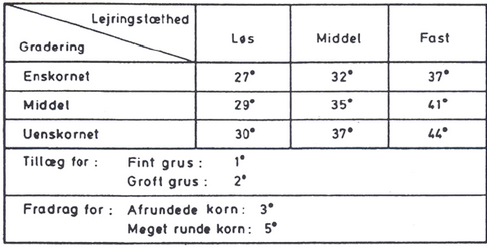
\includegraphics[width=1.2\textwidth]{billeder/friktionsvinkel.png}
		\caption{Friktionsvinkel \citep[ s. 170]{geoteknik}}
		\label{fig:friktionsvinkel}
	\end{minipage}\hfill
\end{figure}

\section{Bæreevne for fundamentet}
Til bestemmelse af bæreevnen af fundamentet benyttes formlen:
\begin{center}
	$\frac{R}{A} = \frac{1}{2} \gamma  b' N_\gamma s_\gamma i_\gamma + q' N_q s_q i_q d_q + c' N_c s_c i_c d_c$
\end{center}

Der beregnes ikke kohæsion, fordi den der næsten ingen kohæsion er imellem sandkornene og dermed betragtes som værende 0. Derfor medregnes $c'*N_c*s_c*i_c*d_c$ -leddet ikke.

\begin{itemize}
	\item[-] R: effektiv lodret bæreevne
	\item[-] A: effektiv areal
	\item[-] $\gamma$: rumvægt for sand - vand, som sættes til $20\frac{kN}{m^3} - 10\frac{kN}{m^3}$
	\item[-] $b'$: effektive bredde
	\item[-] $N_{\gamma}$ og $N_q$: bæreevnefaktor
	\item[-] $s_\gamma$ og $s_q$: formfaktor
	\item[-] $i_\gamma$ og $i_q$: hældningsfaktor
	\item[-] $q'$: effektiv lodret overlejringstryk ved FUK
	\item[-] $d_q$: dybdefaktor
\end{itemize}

Alle værdier pånær $b'$ kan bestemmes, således $b'$ til sidst kan bestemmes.
\newline
\newline
I og med der intet moment er i understøtningen, er hele bredden af fundamentet effektiv og dermed ikke excentrisk. Fra resultanten af alle lodrette kræfter i fundamentunderkanten, V, fås en belastning, og for at fundamentet kan holde, skal R mindst være lige så stor som V.
\newline
\newline
Da det ikke altid kan sikres, at jorden ved siden af fundamentet forbliver intakt, ses der normalt bort fra dybdefaktoren, og sættes $d_q$ til 1.
\newline
\newline
Arealet kan bestemmes, når det antages for at være kvadratisk, og da der intet moment er i understøtningen er $b'=b$ og arealet er givet ved $A=b^2$.
\newline
\newline
Formfaktorerne bestemmes:
\begin{center}
	$s_\gamma = 1 - 0,\!4 \frac{b'}{l'} = 1 - 0,\!4  \frac{b'}{b'} = 1 - 0,\!4 = 0,\!6$
\end{center}

\begin{center}
	$s_q = 1 + 0,\!2 \frac{b'}{l'} = 1 + 0,\!2 \frac{b'}{b'} = 1 + 0,\!2 = 1,\!2$
\end{center}

Hældningsfaktoren, $i_q$, beregnes ved:
\begin{center}
	$i_q = (1 - \frac{H}{V + A c' cot(\varphi)'})^2$
\end{center}

\begin{itemize}
	\item[-] H: resultanten for alle vandrette kræfter i fundamentunderkanten, FUK, som sættes til 133,08 kN
	\item[-] V: resultanten for alle lodrette kræfter i fundamentunderkanten, FUK, som sættes til 535,17 kN
\end{itemize}

Da $c'$ ikke anvendes i dette projekt, sættes denne lig 0 og formlen bliver da:
\begin{center}
	$i_q = (1 - \frac{H}{V})^2$
\end{center}

Hermed kan $i_q$ bestemmes:
\begin{center}
	$i_q = (1 - \frac{133,\!08 kN}{535,\!17 kN})^2 = 0,\!56$
\end{center}

Hældningsfaktoren, $i_{\gamma}$, bestemmes:
\begin{center}
	$i_{\gamma} = i_q^2 = (0,\!56)^2 = 0,\!32$
\end{center}

Det lodrette overlejringstryk ved FUK, $q$, bestemmes, når fundamentet antages at have en højde på 0,8 m (se Figur \ref{fig:hihi}) og der kun regnes for $q_{ude}$, ved:
\begin{center}
	$q = h_1 \gamma + h_2 (\gamma_{sand} - \gamma_{vand})$
\end{center}

\begin{itemize}
	\item[-] $h_1$: længden ned til grundvandsspejlingen, som er 0,8 m
	\item[-] $\gamma$: henholdsvis rumvægten for sand og vand
	\item[-] $h_2$: længden fra grundvandsspejlingen ned til fundamentunderkanten, FUK som er 2,8 m
\end{itemize}

$q$ bestemmes:
\begin{center}
	$q = 0,\!8 m \cdot 20\frac{kN}{m^3} + 2 m (20\frac{kN}{m^3} - 10\frac{kN}{m^3}) = 36,\!00 \frac{kN}{m^2}$
\end{center}

\begin{figure}[htbp]
	\centering
	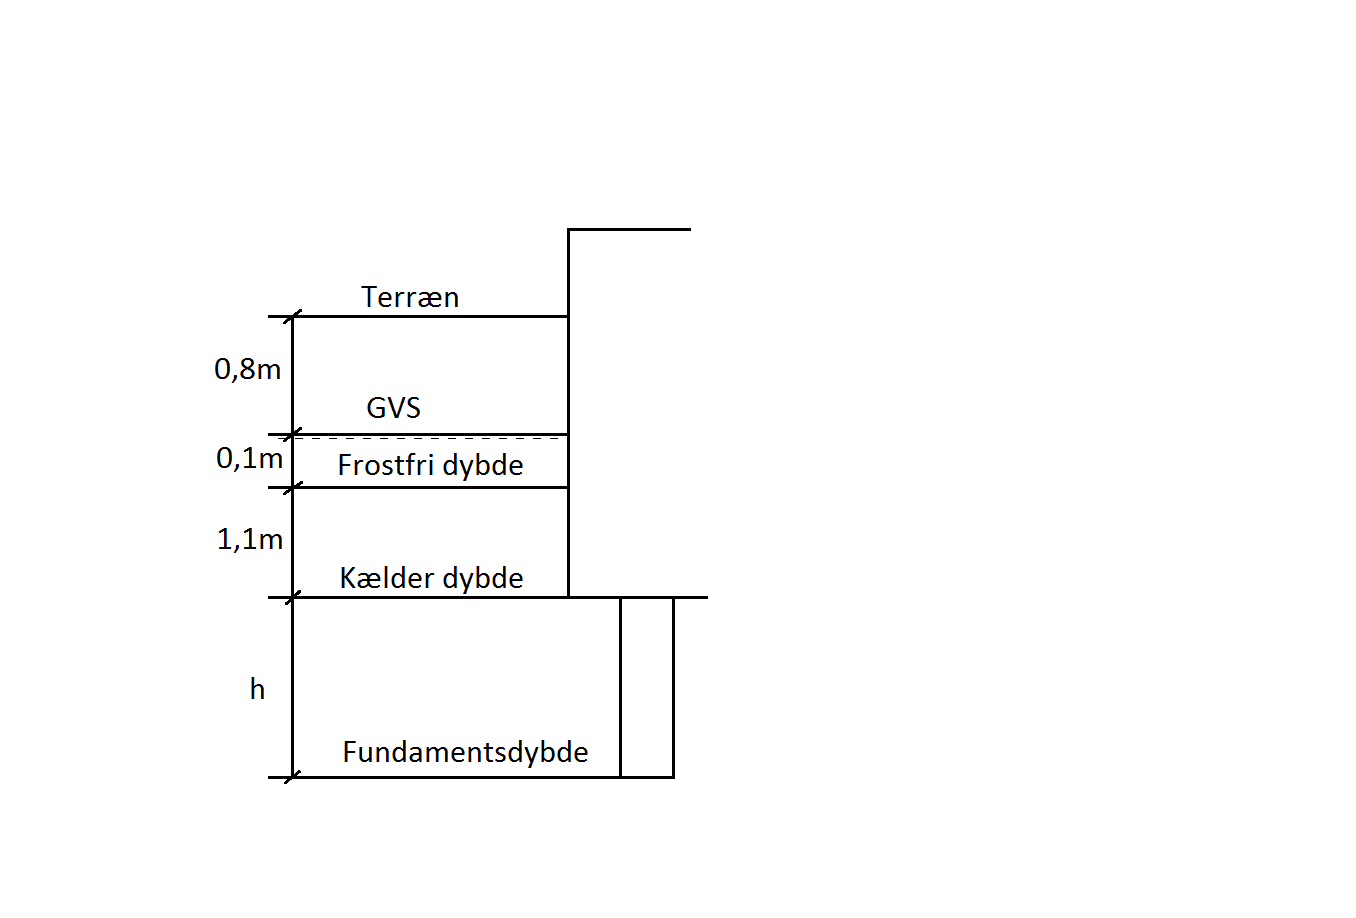
\includegraphics[width=0.4\textwidth]{billeder/fundamentsdybde.png}
	\caption{Fundament}
	\label{fig:hihi}
\end{figure}

Bæreevnefaktorerne bestemmes, når friktionsvinklen $\varphi = 32,\!33$:
\begin{center}
	$N_q = e^{\pi Tan(\varphi)} \frac{1 + Sin(\varphi)}{1 - Sin(\varphi)} = e^{\pi Tan(32,\!33)} \frac{1 + Sin(32,\!33)}{1 - Sin(32,\!33)} = 24,\!08$
\end{center}

\begin{center}
	$N_\gamma = \frac{1}{4}((N_q - 1)Cos(\varphi))^\frac{3}{2} = \frac{1}{4}((24,\!08 - 1)Cos(32,\!33))^\frac{3}{2}=21,\!54$
\end{center}

Bredden $b'=b$ kan nu bestemmes: 
\begin{center}
	$\frac{R}{A} = \frac{1}{2} \gamma b' N_\gamma s_\gamma i_\gamma + q' N_q s_q i_q d_q \leftrightarrow \frac{V}{b^2} = \frac{1}{2} \gamma b' N_\gamma s_\gamma i_\gamma + q' N_q s_q i_q d_q \leftrightarrow \frac{535,\!17 kN}{b^2} = \frac{1}{2}\cdot 10 \frac{kN}{m^3}\cdot b\cdot 21,\!54\cdot 0,\!6 \cdot 0,\!3186610841 + 36,\!00 \frac{kN}{m^2}\cdot 24,\!08 \cdot 1,\!2 \cdot 0,\!56 \cdot 1) = 0,\!94 m$
\end{center}

Dermed skal alle fire sider på fundamentet være 0,94 m hver.
\newline
\newline
Efter bredden af fundamentet er bestemt, bør der ses på anvendelses- og brudgrænser, for at sikre mod eventuelle deformationer og brud. Anvendelsesgrænsen anvendes, når der kigges på stivhedsgraden i jorden. Hvis jordens stivhed ikke er tilstrækkelig, risikerer fundamentet at sætte sig uhensigtsmæssigt. Det skal sikres, at fundamentet passer med konstruktionens formål, men dette afhænger af bygherrens ønske. 
\newline \indent{     }  Stivheden af jorden testes ved at lægge tryk på jorden, og herudfra lave en arbejdskurve, hvor der undersøges stivheden af jorden.   
\newline \indent{     }  Når jord påvirkes af en vertikal kraft, komprimeres jorden lodret, indtil det ikke kan opholdes og derfor skubber ud ad i en brudform. Brudgrænsetilstanden regnes for at se, om jorden kan holde til belastningen fra bygningen. Dette bestemmes via brudanalyse, hvor jordtrykket, der vil skubbe med reaktionen, skal være mindre end jordtrykket, som skubber mod reaktionen. Disse kaldes henholdsvis den drivende- og den stabiliserende kraft. Brudformen afhænger af materialet. For sand er friktionsvinklen afgørende, og for ler er kohæsionen afgørende for styrken. Ler er mere afrundede cirkel, mens spiralerne for sand er fladere. 
\newline \indent{     }  På Figur \ref{fig:haha} ses et eksempel for sand, hvilket viser, hvordan scenariet udspiller sig for sandets spiral. For at bestemme den stabiliserende kraft, opdeles sandet i geometriske områder. På den drivende del bliver fundamentet og dens vægt lagt sammen med vægten af sand samt den vertikale kraft. Den stabiliserende kraft skal være større end den drivende kraft, for at der ikke opstår brud. Der laves brudformer rundt om alle punkter, for at sikre mod brudtilfælde. 

\begin{figure}[htbp]
	\centering
	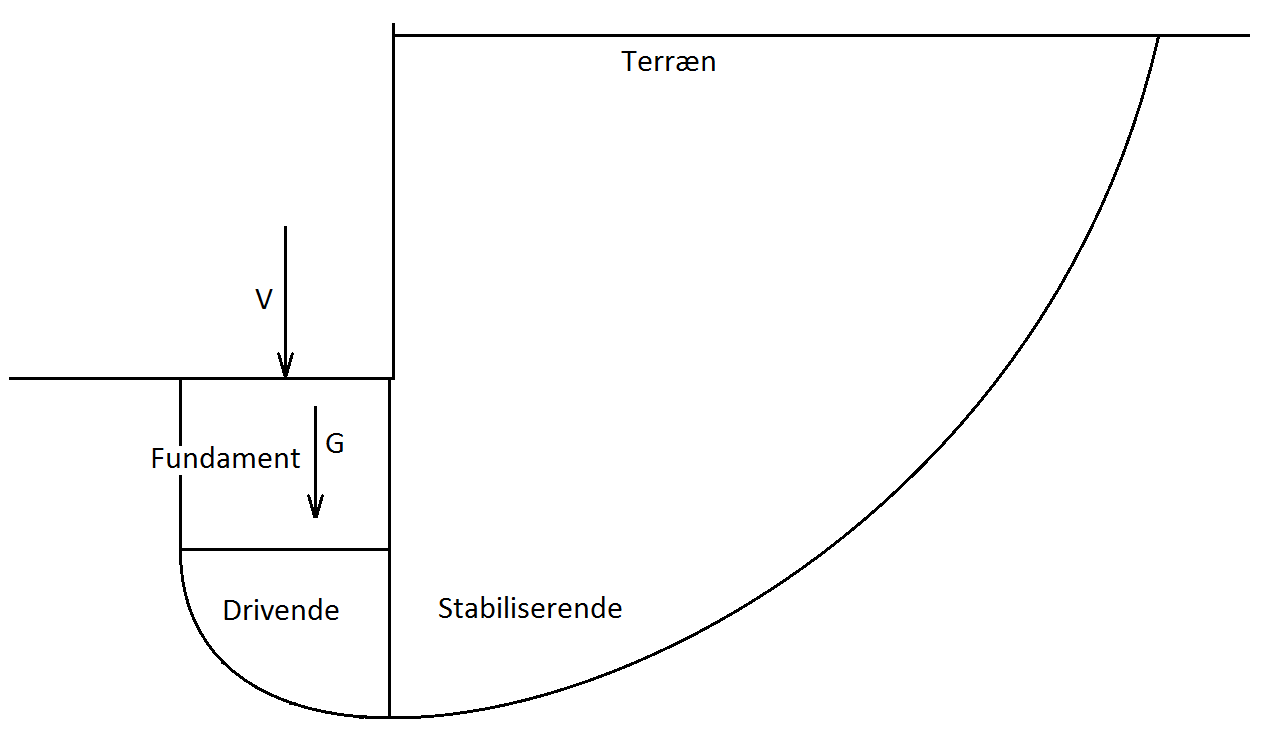
\includegraphics[width=0.5\textwidth]{billeder/spiral.png}
	\caption{Spiral}
	\label{fig:haha}
\end{figure}

\section{Delkonklussion}
Aalborgs geologi er analyseret i denne rapport. Selvom jorden i Aalborg primært består af Aalborgler arbejdes der med boreprofiler fra Hals/Hou, da disse hovedsageligt består af sand. Dette giver mulighed for at benytte direkte fundering. I et laboratorium er der udført fire forsøg med baskapsand fra Sverige, som antages at være sand fra Hals/Hou området, så disse stemmer overens med boreprofilerne. Formålet med de fire forsøg er, at skønne friktionsvinklen, som er $32,\!33^{\circ}$. Der ønskes at lave et punktfundament for hver søjle, som skønnes til at være XX m i både bredden og længden, for at fundamentet har tilstrækkelig bæreevne.

%% Afrunding %%

\chapter{Konklusion}
 Aalborg Kommune har igennem den nuværende kommuneplan en målsætning om, at blive Nordjyllands Vækstdynamo og være en by med fokus på udvikling af studieliv, erhverv, kultur m.m. Blandt et af kommunens fem fokuspunkter er “Aalborg - den attraktive storby”, som omhandler Vækstaksen, der beskriver et område i Aalborg, hvor der er stort fokus på byens udvikling og vækst.
 \newline \indent{     }  De seneste 10 års udvikling på Aalborg Havnefront har givet øget fokus på udviklingen i netop dette område. Strøybergs Palæs beliggenhed ved Aalborg Havnefront, i den mest centrale del af Vækstaksen, gør, at tilbygningen har gode vilkår i forbindelse med vækst og udvikling, og tilbygningen kan blandt andet bruges til beboelse og erhvervslokaler, som kan tiltrække nye virksomheder til området. Strøybergs Palæ er en lille del af Aalborgs udvikling, men en tilbygning må formodes ikke at have en central betydning for Aalborgs udvikling, idét tilbygningen kun er en lille del af Vækstaksen.
 \newline \indent{     }  Strøybergs Palæ er underlagt Lokalplan 1-1-107, der beskriver to byggefelter til bygningen. Der er udarbejdet en tilbygning for delområde B, hvor ny bebyggelse må opføres i 3 etager, samt en tagetage og kælder. Med udgangspunkt i Lokalplan 1-1-107 er bygningens størrelse og dimensioner bestemt. Hertil er der opstillet et statisk system, og der er valgt at indsætte tre stålrammer, hvor der dimensioneres efter den midterste ramme.
 \newline \indent{     }  Tilbygningens stålprofiler er dimensioneret ud fra ståltype S235 med profil nr. 450, samt ud fra de permanente og variable laster der virker på tilbygningen; egenlast, jordlast, vindlast, snelast og nyttelast. Herudfra er tilbygningens brud- og anvendelsesgrænsetilstand bestemt.
 \newline \indent{     }  Ud fra spændingstilstanden kan det konkluderes, at tilbygningen har en tilstrækkelig bæreevne, idet der fås en maksimal spænding på 100,51 MPa mod en flydespænding på 204,54 MPa. 
 \newline \indent{     }  For anvendelsesgrænsetilstanden er udbøjningen bestemt for tre af konstruktionens stålstænger. Her er den vandrette udbøjning bestemt til 1762,89 mm, mens den lodrette udbøjning er bestemt til 24,92 mm. Denne overskrider de anbefalede værdier for udbøjning af bærende konstruktioner, hvilke for vandret er 36 mm og lodret 15,63 mm.
 \newline \indent{     }  Tilbygningens fundament er dimensioneret ud fra Aalborgs geologi. Aalborgs undergrund er primært bestående af Aalborgler og funderingen til Strøybergs Palæ burde dermed være pælefundering. I dette projekt var ønsket at arbejde med direkte fundering, og derfor er der anvendt boreprofiler fra Hals, hvor undergrunden primært består af senglacialt sand, hvilket antages at være boreprofilerne fra området ved Strøybergs Palæ.
 \newline \indent{     }  De udførte laboratorieforsøg, hvor formålet er at bestemme friktionsvinklen, er udført på baskarpsand fra Sverige, der antages at være sandet fra boreprofilerne. Ud fra de fire forsøg er friktionsvinklen skønnet til $32,33^{\circ}$, der anvendes i videre beregninger af fundamentets størrelse. Der laves et punktfundament for hver søjle i det statiske system, med en længde og bredde på 0,94 m.


%%%% Kilder %%%%

\begingroup
	\raggedright
	\bibliography{bibtex/litteratur}							% Litteraturlisten inkluderes
\endgroup



%%%% Appendiks %%%%

\appendix														% Appendiks/bilag start - giver chapter bogstaver i stedet for tal
\clearforchapter												% Sikrer at pagestylen aktiveres paa den rigtige side
\phantomsection													% Kunstigt afsnit, som hyperlinks kan 'holde fast i'
\pdfbookmark[0]{Appendiks}{appendiks}							% Tildeler en klikbar bookmark til den endelige PDF

%% Indstillinger for appendiks (deaktiveret med "%") %%

%\pagestyle{empty}												% Sidehoved/-fod for standardsider aendres til tom for appendiks
%\aliaspagestyle{chapter}{empty}								% Sidehoved/-fod for kapitelsider aendres til tom for appendiks
%\settocdepth{chapter}											% Kun kapitel-niveau vises i ToC
%\addtocontents{toc}{\protect\cftpagenumbersoff{chapter}}		% Sidetal for kapitler fjernes i ToC

%% Filer til appendiks %%



%%%% Bilag %%%%

\chapter{Beregning af peakhastighedstrykket}
Nedenfor gives et beregningseksempel af peakhastighedstrykket, $q_p$, for taget med vindretning fra vest. Fremgangsmåden for vindretningerne øst og nord er identisk med nedenstående eksempel, blot med andre værdier fra de samme kilder som anvendes i eksemplet, da vindretning og højden ændres.
\newline
\newline
Den maksimale belastning fra vinden, peakhastighedstrykket $q_p$, bestemmes ved:
\begin{equation}
	q_p(z_e)=[1+7I_v(z_e)]\frac{1}{2}pv_m^2(z_e)
\end{equation}
\begin{itemize}
	\item[-] $I_v$: Vindturbulens
	\item[-] $\rho$: Densiteten for luft ved $20^{\circ}$, $1,\!25 \frac{\text{kg}}{\text{m}^3}$
	\item[-] $v_m$: Middelvindhastigheden
\end{itemize}
For at bestemme peakhastigheden, beregnes først vindturbulens $I_v(z)$ samt middelvindhastigheden $v_m$.
\newline
\newline
Vindturbulens, $I_v(z)$, bestemmes ved:
\begin{equation}
	I_v(z)=\frac{\sigma_v}{V_m(z)}=\frac{k_1}{c_0(z) \text{ln}(\frac{z}{z_0})}
\end{equation}
\begin{itemize}
	\item[-] $k_1$: Turbulensfaktor, sættes til $1,\!0$ \citep[ kapitel 4.4]{EU91}
	\item[-] $c_0(z)$: Orografifaktoren, som sættes til $1,\!0$ \citep[ kapitel 4.3.1]{EU91}
	\item[-] $z$: Højden, som med taget er 19 m
	\item[-] $z_0$: Ruhedslængde, som sættes til $1,\!0$ for terrænkategori IV \citep[ tabel 4.1 kapitel 4.3.2]{EU91}
\end{itemize}
Vindturbulensen bestemmes til:
\begin{equation}
	I_v(z)=\frac{1,\!0}{1,\!0\cdot \text{ln}(\frac{19}{1,0})}=0,\!34
\end{equation}

Middelvindhastigheden, $v_m$, bestemmes ved:
\begin{equation}
	v_m(z)=c_r(z)c_0(z)v_b
\end{equation}

\begin{itemize}
	\item[-] $c_r(z)$: Ruhedsfaktor
	\item[-] $v_b$: Basisvindhastigheden
\end{itemize}
Til at bestemme middelvindhastigheden, beregnes basisvindhastigheden samt ruhedsfaktoren.
\newline
\newline
Basisvindhastigheden, $v_b$, bestemmes ved:
\begin{equation}
	v_b=c_{dir}c_{season}v_{b,0}
\end{equation}
\begin{itemize}
	\item[-] $c_{dir}$: Retningsfaktor, som sættes til $1,\!0$ ved vind fra vest \citep[ tabel 1a kapitel 4.2]{EU91}
	\item[-] $c_{season}$: Årstidsfaktor, som sættes til $1,\!0$ \citep[ tabel 1b kapitel 4.2]{EU91}
	\item[-] $v_{b,0}$: Grundværdi for basisvindhastigheden, som sættes til 24 $\frac{\text{m}}{\text{s}}$ \citep[ kapitel 4.2]{EU91}
\end{itemize}
Basisvindhastigheden bestemmes til:
\begin{equation}
	v_b=1,\!0\cdot 1,\!0\cdot 24 \frac{\text{m}}{\text{s}}=24 \frac{\text{m}}{\text{s}}
\end{equation}

Ruhedsfaktor, $c_r(z)$, bestemmes ved:
\begin{equation}
	c_r(z)=k_r \text{ln}(\frac{z}{z_0})
\end{equation}
\begin{itemize}
	\item[-] $k_r$: Terrænfaktor
\end{itemize}

Terrænfaktoren, $k_r$, bestemmes ved:
\begin{equation}
	k_r=0,\!19\cdot (\frac{z_0}{z_{0,II}})^{0,07}
\end{equation}

\begin{itemize}
	\item[-] $z_{0,II}$: Værdi for ruhedslængde for terrænkategori II, som sættes til $0,\!05$ \citep[ kapitel 4.3.2]{EU91}
\end{itemize}

\begin{equation}
	k_r=0,\!19\cdot (\frac{1,\!0}{0,\!05})^{0,07}=0,\!234
\end{equation}
Ruhedsfaktor bestemmes til:
\begin{equation}
	c_r(z)=0,\!234\cdot \text{ln}(\frac{19}{1,\!0})=0,\!690
\end{equation}
Middelvindhastigheden bestemmes til:
\begin{equation}
	v_m(z)=0,\!690\cdot 1,\!0\cdot 24 \frac{\text{m}}{\text{s}}=16,\!569 \frac{\text{m}}{\text{s}}
\end{equation}
Peakhastighedstrykket $q_p$ i højden z, bestemmes til:
\begin{equation}
	q_p(z_e)=[1+7\cdot 0,\!340]\cdot \frac{1}{2}\cdot 1,\!25 \frac{\text{kg}}{\text{m}^3}\cdot (16,\!569 \frac{\text{m}}{\text{s}})^2=0,\!579 \frac{\text{kN}}{\text{m}^2}
\end{equation}
\chapter{Forsøg: Vandindhold}

\textbf{Formål}
\newline
Formålet med dette forsøg er at finde vandindholdet, w, i en jordprøve. Vandindholdetn er defineret som, jordens vægttab i \% af tørvægten ved tørring i et varmeskab ved en temperatur på 105$^{\circ}$C til konstant vægt er opnået.
\newline
\newline
\textbf{Apperaturliste}
\begin{itemize}
\item[-] Vægt, vejenøjagtighed 0.01 g
\item[-] Skål i varme- og korrosionsbestandigt materiale
\item[-] Tørreskab, temperatur til 105$^{\circ}$C
\end{itemize}

\textit{Tabel 1}

%Tabel skal være her!!%

\textbf{Fremgangsmåde}
\newline
Først findes en ren og tør foliebakke vejes, og vægten noteres som \textit{sk.} Efterfølgende udtages en passsende mængde jord, jf. tabel 1, og anbringes i foliebakken, og det hele vejes omgående sammen, og noteres som \textit{W+sk}.
\newline
Foliebakken anbringes nu i tørreskabet ved 105$^{\circ}$C, og tørres fra fredag til mandag (Normalt tørres det i 24 timer, da konstant vægt normalt er opnået eftter dette tidsrum). Efter tørringen sættes foliebakken til afkåling i vacuumekssikator til rumtemperatur er opnået. Den afkølede foliebakke med den nu tørre jordprøve vejes,\textit{$W_{s}+sk$}


%Resultat tabel indsættes%

\textbf{Beregninger}
\begin{center}
\newline
\textit{Beregninger udføres på følgende måde:}
\newline
$w=\frac{W_w}{W_s}*100\%=\frac{(W+sk)-(W_s+sk)}{(W_s+sk)-sk}*100\%$
\newline
\textit{Vandindholdet regnes nu forsøg 2:}
$w=\frac{(81,02)-(80,99)}{(80,99)-3,07}*100\%=0,038501\%$
\newline
\textit{Vandindholdet regnes nu for forsøg 2:}
\newline
$w=\frac{(89,83)-(89,79)}{(89,79)-3,11}*100\%=0,046147\%$
\end{center}
\newline
\newline
\textbf{Fejlkilder}
\newline
Forskelligheden i de 2 prøveforsøg kan skyldes brugen af 2 forskellige vægte med forskellige størrelse usikkerheder. En anden fejlkilde er at størrelserne på prøverne er forskellige vægten er med en difference på 8,81 g, samt der ikke er taget højde for tabel 1, så mængden af prøvemateriale sker ud fra anbefaling.
\newline
\newline
\textbf{Delkonklusion}
\newline
Udfra de opnåede resultater kan det konkluderes at 


\chapter{Bilag B}
\section{Sigteanalyse}
\textbf{Formål}
\newline
Formålet med forsøger er at bestemme jordkornenes vægtmæssige fordeling efter størrelse i sand- og grusfraktion, for at beregne uensformighedstallet for jorden, der skal bruges i de videre beregninger af friktionsvinklen. 
\newline
\newline
Velsorteret: U<2
\newline 
Sorteret: 2<U<3,5
\newline
Ringe sorteret: 3,5<U<7
\newline
Usorteret: U>7
\newline
\newline
\textbf{Apparaturliste}
\begin{itemize}
	\item[-] Sigter med mindst maskevidde på 0,063 mm
	\item[-] Rystemaskine
	\item[-] Vægt med vejenøjagtighed på 0,01 g
	\item[-] Sigtebørste
	\item[-] Skåle i korrosion bestandigt materiale
\end{itemize}
\textbf{Fremgangsmåde}
\newline
Ved en sigteanalyse kan der både udføres en grovsigtning og en finsigtning. Grovsigtningen udføres, hvis materialet vurderes til at have partikler over 16 mm. I dette forsøg er der kun udført en finsigtning, da partiklerne vurderes til at være mindre en 16 mm. Sigtningen er udført på sigter fra 0,063 mm til 2 mm (sigtemålene kan ses i tabellen over resultaterne). 
\newline \indent{     }   Først rengøres hver enkelt sigte forsigtigt med sigtebørste, og herefter samles sigterne forløbende fra den største maskevdde øverst til bunden nederst. Det afmålte materiale hældes på sigten med den største maskevidde på 2 mm, hvorefter sigtetårnet placeres i rystemaskinen og sigtes i 20 minutter.
\newline \indent{     }   Sigteresterne i hver enkelt sigte overføres til skåle og vejes. Hver sigte placeres med bunden opad på et stort stykke papir, og der fejes let på bagsiden, således materialet der sidder fast i maskerne løsnes.
\newline \indent{     }   Alle resultaterne skrives ind i nedenstående tabel, hvor det procentvise gennemfald i hver sigte beregnes ved $gennemfald [\%] = \frac{gennemfald [g]}{samlet prøve [g]}\cdot 100 [\%]$. Herefter optegnes en sigtekurve over resultaterne med det procentvise gennemfald af y-aksen i aritmisk skala, og kornstørrelse af x-aksen i logaritmisk skala. Herpå aflæses de to punkter der ligger mellem henholdsvis 10\% og 60\%, og der laves lineær regression imellem de to punkter. Herudfra kan 10\%-fraktilen, $d_{10}$, og 60\%-fraktilen, $d_{60}$, beregnes. Disse bruges til at udregne uensformighedstallet $U = \frac{d_{60}}{d_{10}}$
\newline
\newline
\textbf{Resultater}
\newline
Tabel over resultater for det første udførte forsøg:
\newline
\newline
Tabel over resultater for det andet udførte forsøg:
\newline
\newline
\textbf{Beregninger}
\newline
\underline{Forsøg 1}
\newline
\newline
HER INDSÆTTES SIGTEKURVE FOR FORSØG 1
\newline
\newline
For at finde 10\%-fraktilen er der lavet lineær regression imellem sigte med maskestørrelse 0,075 mm og 0,125 mm, hvor følgende ligning fremgår: 

\begin{center}
	$y=862.42\cdot x - 63.223$
\end{center}

For at finde 60\%-fraktilen er der lavet lineær regression imellem sigte med maskestørrelse 0,125 mm og 0,15 mm, hvor følgende ligning fremgår:

\begin{center}
	$y=937.12\cdot x - 72.56$
\end{center}

Henholdsvis 10\%-fraktilen og 60\%-fraktilen er beregnet til:



\underline{Forsøg 2}
\newline
\newline
HER INDSÆTTES SIGTEKURVE FOR FORSØG 2






\chapter{Forsøg: Kornvægtfylde}

\textbf{Apparaturliste}
\begin{itemize}
\item[-] Pyknometer
\item[-] Bægerglas
\item[-] Termometer med nøjagtighed $0,\!1^{\circ}$C
\item[-] Vægt med vejenøjagtighed på 0,001 g
\item[-] Tørreskab, temperatur til 105$^{\circ}$C
\end{itemize}

\textbf{Fremgangsmåde}
\newline
Dette forsøg laves med friktionsjord (tør metode). Der udtages en prøve af 150 g tørstof, og dette placeres i et 500 ml pyknometer. Pyknometeret fyldes ca. halvt op med luftfrit demineraliseret vand, og der drejes på pyknometeret for at undgå luftbobler. Derefter hældes der vand i, indtil vandet flyder over, når proppen sættes i. Proppen sættes i, og der sørges igen for, at der ikke er luftbobler til stede. Pyknometeret med materiale, vand og prop vejes og kaldes $W_{1}$, og beregnes altså ved $W_1 = W_{pyk} + W_s + W_{vand}$. Herefter måles temperaturen i pyknometeret, og temperaturen noteres. Dernæst aflæses $W_{2}$ i et kalibreringsskema og noteres $p_w^t$.
\newline
\newline
\textbf{Resultater}
\begin{center}
	\begin{tabular}{ |c|c|c| } 
		\hline
		 & Forsøg 1 & Forsøg 2 \\	\hline
		Pyknometer nr. & 103 & 100 \\	\hline
		$W_1$ [g] & 728,89 & 709,40 \\	\hline 
		Temperatur [$^{\circ}$C] & 22 & 23 \\ \hline
		$W_2$ [g] & 641,164 & 615,967 \\	\hline
		$W_s$ [g] & 161,27 & 150,06 \\	\hline
		$\rho_{w}^t$ [$\frac{g}{mL}$] & 0,998 & 0,998 \\	\hline
		$d_s$ [$\frac{g}{m^3}$] & 2,188 & 2,644	\\	\hline	
	\end{tabular}
\end{center}

\textbf{Fejlkilder}
\newline
En fejlkilde ved dette forsøg er luftbobler i pyknometeret. Derudover var det en del af forsøget at benytte en vacuumekssikator, men grundet manglende tid blev dette trin sprunget over. En anden fejlkilde er, at der kan være forskellige temperaturer i pyknometeret, og udover disse fejlkilder er der også måleusikkerheder, som eksempelvis når der tørstof og pyknometer skulle vejes eller temperaturen skulle måles. 
Ved forsøg 1 blev der vejet forkert og dette antages at være årsagen til det misvisende resultat.
\chapter{Forsøg: Løs og fast lejring}

\textbf{Formål}
\newline
Formålet med dette forsøg er at bestemme hvor meget materiale der er tilbageholdt, som bruges til at finde lejringstætheden og poretallet af materialet.
\newline
\newline
\textbf{Apperaturliste}
\begin{itemize}
	\item[-] Lille cylinder
	\item[-] Tragt
	\item[-] Stållineal
	\item[-] Stamper passende til valgte cylinder
	\item[-] Specialskydelære passende til valgte cylinder
	\item[-] Vægt, vejenøjagtighed $0,\!01$ g
	\item[-] Sigte med maskevidde på 5 mm 
\end{itemize}

\textbf{Fremgangsmåde}
\newline
\underline{Løs lejring}
\newline
En delprøve af jordprøven er taget fra til forsøgende. Der startes med at placere cylinderen i en bakke. I cylinderen anbringes sigten. Så hældes materialet forsigtigt  op i sigten. Det skal glide ned ad kanten på sigten og videre i cylinderen. Der bruges tilstrækkeligt materiale at cylinderen kan fyldes helt op og så noget går over kanten. Sigten hæves nu forsigtigt op ad cylinderen. Det skal gøres over ca. et minut  i en jævn og flydende bevægelse. Når alt materialet er blevet hældt i cylinderen fjernes toppen med en stållineal således at materialet flågter med cylinderens overflade. Ved siden af cylinderet slås der hårdt to gange i bordet, så materialet sætter sig. Materiale der skulle befinder sig på ydersiden af cylideren børstes væk. Herefter vejes cylinderen og materialet, \textit{Cyl+Ws}. Cylinderen tømmes for materiale , børstes og vejes \textit{Cyl}.
\newline
\newline
\underline{Fast lejring}
\newline
Samme delprøve fra løs lejring bruges til fast lejring. Til fast lejring bliver cylinderet fyldt ad fem gange. Mellem hver fyldning, bliver materialet jævnet ud med en stållineal derefter stampes der. Antallet af slag stiger for hvert lag der kommer i. Stamperen holdes lodret i cylinderen. Faldloddet føres op til stopklodsen for at slippes og foretage frit fald. For hvert tiende slag tages stamperen for at der ikke fastklemmes materiae mellem stamperen og cylinderetsvæg. Stamperens fod børstes for materiale som eventuelt skulle være presset mod. Inden det sidste lag skal stampes skal der være ca. 0.5 cm fra materialet og op til toppen af cylinderet. Efter sidste stampning fjernes materiale der skulle sidde fast på stamperen og skydelæren sættes på kanten af cylinderet. Højden ned til materialet måles. Materiale som skulle være på ydersiden af cylinder børstes væk og cylinderen med materialet vejes \textit{Cyl+Ws}. Materialet fjernes og cylinderen bliver børstes og vejet \textit{Cyl}.
\newline
\newline
\textbf{Resultater for løs lejring}
\begin{center}
	\begin{tabular}{ |c|c|c| } 
		\hline
		Prøve nr & 1 & 2 \\	\hline 
		Areal [$cm^2$] & 10,0 & 10,0 \\ \hline
		Højde [cm] & 7,0 & 7,0 \\ \hline
		Volume [$cm^3$] & 70 & 70 \\ \hline
		Cyl + $W_s$ [g] & 340,45 & 340,46 \\ \hline
		Cyl [g] & 241,99 & 241,99 \\ \hline
		$W_s$ [g] & 98,55 & 98,47 \\ \hline
		e & 0,873 & 0,875 \\ \hline
	\end{tabular}
\end{center}

\begin{center}
	\begin{tabular}{ |c|c|c| } 
		\hline
		Prøve nr & 3 & 4 \\	\hline
		Areal [$cm^2$] & 10,0 & 10,0 \\ \hline
		Højde [cm] & 7,0 & 7,0 \\ \hline
		Volume [$cm^3$] & 70 & 70 \\ \hline
		Cyl + $W_s$ [g] & 340,50 & 337,52 \\ \hline
		Cyl [g] & 241,99 & 241,99 \\ \hline
		$W_s$ [g] & 98,51 & 98,57 \\ \hline
		e & 0,874 & 0,873\\ \hline
	\end{tabular}
\end{center}

\textbf{Resultater for fast lejring}
\begin{center}
	\begin{tabular}{ |c|c|c| } 
		\hline
		Prøve nr & 1 & 2 \\	\hline 
		Areal [$cm^2$] & 10,0 & 10,0 \\ \hline
		Højde [cm] & 6,5 & 6,575 \\ \hline
		Volume [$cm^3$] & 65 & 65,75 \\ \hline
		Cyl + $W_s$ [g] & 349,48 & 349,31 \\ \hline
		Cyl [g] & 241,99 & 238,95 \\ \hline
		$W_s$ [g] & 107,49 & 110,36 \\ \hline
		e & 0,595 & 0,571 \\ \hline
	\end{tabular}
\end{center}

\begin{center}
	\begin{tabular}{ |c|c|c| } 
		\hline
		Prøve nr & 3 & 4 \\	\hline
		Areal [$cm^2$] & 10,0 & 10,0 \\ \hline
		Højde [cm] & 6,42 & 6,355 \\ \hline
		Volume [$cm^3$] & 64,2 & 63,55 \\ \hline
		Cyl + $W_s$ [g] & 346,55 & 345,75 \\ \hline
		Cyl [g] & 238,95 & 238,95 \\ \hline
		$W_s$ [g] & 107,6 & 106,8 \\ \hline
		e & 0,573 & 0,569 \\ \hline
	\end{tabular}
\end{center}

\textbf{Fejlkilder}
\newline
I forsøggentagelse 2 i fast lejring blev der fyldt for meget materiale i cylinderen. Derfor er der taget noget ud efter de 80 slag og herefter er der givet 10 ekstra slag, hvilket kan give anledning til et varierende resultat. Det ses også, at resultat $W_s$ varierer lidt i forhold til de resterende forsøg.

%\phantomsection												% Kunstigt afsnit, som hyperlinks kan 'holde fast i'
%\addcontentsline{toc}{chapter}{Bilag A \ Navn} 				% Manuelle indgange i indholdsfortegnelsen (naar \includepdf bruges)

%\includepdf[pages={x-y}]{filnavn}								% Inkluder eksterne bilag med \includepdf[pages={x-y}]{filnavn}

\end{document}													% Slutter dokumentet - obligatorisk